\documentclass{patmorin}
\listfiles
\usepackage{pat}
\usepackage[T1]{fontenc}
\usepackage[utf8]{inputenc}
\usepackage{comment}
\usepackage[inline]{enumitem}
\usepackage[normalem]{ulem}

%\piotr{added packages}
\usepackage{mathtools}  % for \DeclarePairedDelimiter
%\piotr{end of added packages}
\usepackage[longnamesfirst,numbers,sort&compress]{natbib}
% \setlength{\bibsep}{0.4ex plus 0.2ex minus 0.2ex}

%% so that cleveref outputs Theorems 3--5
\newcommand{\crefrangeconjunction}{--}
% Use Cref for equations
\crefformat{equation}{#2(#1)#3}
\let\eqref\cref
\crefformat{subsection}{Subsection #2#1#3}
\crefformat{subsubsection}{Subsubsection #2#1#3}

% david proposes the following additions
\renewcommand{\ge}{\geqslant}
\renewcommand{\le}{\leqslant}
\renewcommand{\geq}{\geqslant}
\renewcommand{\leq}{\leqslant}

% For coauthor discussions
\newcommand{\david}[1]{\noindent{\color{orange} DW: #1}}
\newcommand{\vida}[1]{\noindent{\color{pink} VD: #1}}
\newcommand{\pat}[1]{\noindent\textcolor{Magenta}{PaMo: #1}}
\newcommand{\gwen}[1]{\noindent\textcolor{Purple}{GJ: #1}}
\newcommand{\cyril}[1]{\noindent\textcolor{Green}{CG: #1}}
\newcommand{\piotr}[1]{\noindent\textcolor{red}{PiMi: #1}}

\usepackage[mathlines]{lineno}
\setlength{\linenumbersep}{2em}
\linenumbers
% \rightlinenumbers
% \linenumbers
\newcommand*\patchAmsMathEnvironmentForLineno[1]{%
 \expandafter\let\csname old#1\expandafter\endcsname\csname #1\endcsname
 \expandafter\let\csname oldend#1\expandafter\endcsname\csname end#1\endcsname
 \renewenvironment{#1}%
    {\linenomath\csname old#1\endcsname}%
    {\csname oldend#1\endcsname\endlinenomath}}%
\newcommand*\patchBothAmsMathEnvironmentsForLineno[1]{%
 \patchAmsMathEnvironmentForLineno{#1}%
 \patchAmsMathEnvironmentForLineno{#1*}}%
\AtBeginDocument{%
\patchBothAmsMathEnvironmentsForLineno{equation}%
\patchBothAmsMathEnvironmentsForLineno{align}%
\patchBothAmsMathEnvironmentsForLineno{flalign}%
\patchBothAmsMathEnvironmentsForLineno{alignat}%
\patchBothAmsMathEnvironmentsForLineno{gather}%
\patchBothAmsMathEnvironmentsForLineno{multline}%
}

\definecolor{brightmaroon}{rgb}{0.76, 0.13, 0.28}
\definecolor{linkblue}{rgb}{0, 0.337, 0.227}
\newcommand{\defin}[1]{\emph{\textcolor{brightmaroon}{#1}}}
\makeatletter
\def\mathcolor#1#{\@mathcolor{#1}}
\def\@mathcolor#1#2#3{%
  \protect\leavevmode
  \begingroup
    \color#1{#2}#3%
  \endgroup
}
\makeatother
\newcommand{\mathdefin}[1]{\mathcolor{brightmaroon}{#1}}

\setlength{\parskip}{1ex}

% Document-specific commands and math operators
\newcommand{\torso}[2]{{#1}\langle{#2}\rangle}
\DeclareMathOperator{\height}{height}
\DeclareMathOperator{\depth}{depth}
\DeclareMathOperator{\tw}{tw}
\DeclareMathOperator{\pw}{pw}
\DeclareMathOperator{\lca}{lca}
\DeclareMathOperator{\lgg}{\hat{lg}}

%\piotr{some of my macros}
\newcommand{\calG}{\mathcal{G}}
\newcommand{\Oh}{\mathcal{O}}
\newcommand{\calT}{\mathcal{T}}
\DeclarePairedDelimiter{\set}{\{}{\}}

\DeclarePairedDelimiter{\ceil}{\lceil}{\rceil}

\title{\MakeUppercase{\boldmath  Adjacency labelling for proper minor-closed graph classes}}

\author{
 Vida Dujmovi{\'c}\,\footnote{School of Computer Science and Electrical Engineering, University of Ottawa, Ottawa, Canada (\texttt{vida.dujmovic@uottawa.ca}). Research supported by NSERC and a University of Ottawa Research Chair.}
 \qquad
 Gwena\"el Joret\footnote{D\'epartement d'Informatique, Universit\'e libre de Bruxelles, Belgium ({\tt gwenael.joret@ulb.be}). G.\ Joret is supported by the Belgian National Fund for Scientific Research (FNRS) and by the Australian Research Council.}
 \qquad
 Cyril Gavoille\footnote{LaBRI, University of Bordeaux, France (\texttt{gavoille@labri.fr}). This work is supported by the French ANR Projets ENEDISC (ANR-24-CE48-7768-01) and TEMPOGRAL (ANR-22-CE48-0001).}\\[1ex]
 Piotr Micek\footnote{Department of Theoretical Computer Science, Faculty of Mathematics and Computer Science, Jagiellonian University, Kraków, Poland (\texttt{piotr.micek@uj.edu.pl}). Research supported by the National Science Center of Poland under grant UMO-2023/05/Y/ST6/00079 within the WEAVE-UNISONO program.}
 \qquad
 Pat Morin\footnote{School of Computer Science, Carleton University, Ottawa, Canada (\texttt{morin@scs.carleton.ca}). Research supported by NSERC.}
 \qquad
 David~R.~Wood\footnote{School of Mathematics, Monash University, Melbourne, Australia (\texttt{david.wood@monash.edu}). Research supported by the Australian Research Council and by NSERC.}
 }

% \author{Anonymous}

\date{}


\begin{document}
\maketitle


%\david{Suggested title: Optimal adjacency labelling for minor-closed classes of graphs}
%\piotr{I think the shorter version has some elegance. Also, our labelling is optimal up to the lower order term. I would vote to stay with the current title.}
%\pat{I would also keep opti mal out of the title}
% \gwen{What about adding "proper" in front of "minor-closed" in the title?}
% \pat{Sure. Do we prefer proper minor-closed classes of graphs or proper minor-closed graph classes?}
% \gwen{No strong preference, maybe "proper minor-closed graph classes"?}
\begin{abstract}
We show that every proper minor-closed class of graphs admits
a $(1+o(1))\log_2 n$-bit adjacency labelling scheme. Equivalently, for every proper minor-closed class $\mathcal{G}$ and every positive integer $n$ there exists an $n^{1+o(1)}$-vertex graph $U$ such that every $n$-vertex graph in $\mathcal{G}$ is isomorphic to an induced subgraph of $U$.
%\piotr{I thought we decided to not put the comment below.} \david{We previously wrote ``optimal'' without ``up to the lower order term'', which we considered a possible exageration. With ``up to the lower order term'', I like the sentence. }
Both results are optimal up to the lower order term.
%\vida{I would potentially end this sentence here. By saying "recent discovery of ... planar graphs" we may immediately put in PC/ref mind "incremental" and "they just added onto a recent result", before even getting to tell the story}  \pat{I worry a bit about that too.  Without reading the details it might feel like we're just using the Graph Minor Structure Theorem and turning the crank, especially if you know that we can already label $k$-almost-embedded graphs using \cite{dujmovic.esperet.ea:adjacency}.}
%\gwen{I'd prefer too to finish the sentence here.}
%and improve upon a long sequence of results beginning with trees in the 1980s and leading up to the recent discovery of a $(1+o(1))\log n$-bit adjacency labelling scheme for planar graphs.
% \piotr{If we decide to include this sentence than I really suggest to remove the part in brackets.} (and, more generally, apex-minor-free) graphs. \david{I am happy to drop ``(and, more generally, apex-minor-free)''.}
  \end{abstract}

%  \newpage
%  \tableofcontents

  % \newpage
  % \setcounter{page}{1}
  \section{Introduction}
Let $\calG$ be a class of graphs and let $f:\N\to\N$ be a function.
We say that $\calG$ admits an \defin{$f(n)$-bit adjacency labelling scheme} if there exists a function $A:(\set{0,1}^*)^2\to\set{0,1}$ such that for all positive integers $n$, for every $n$-vertex graph $G\in\calG$, there exists a function $\ell: V(G)\to\set{0,1}^*$ such that
$|\ell(v)|\leq f(n)$ for each vertex $v$ in $G$, and such that
for every two vertices $u$, $v$ in $G$,
\[
A(\ell(u),\ell(v))=\begin{cases}
0&\textrm{if $uv\notin E(G)$},\\
1&\textrm{if $uv\in E(G)$}.
\end{cases}
\]

In this paper we prove the following result. (All logarithms are in base $2$.)

\begin{thm}
\label{main_result}
Every proper minor-closed class of graphs admits
a $(1+o(1))\log n$-bit adjacency labelling scheme.
\end{thm}


Note that all the dependence on the fixed proper minor-closed class in~\cref{main_result} is in the $o(\log n)$ term. Also, \cref{main_result} is optimal up to the $o(\log n)$ term,
which is $\Oh\left((\log n)^{3/4}\right)$.
The proof of~\cref{main_result} is constructive. For every fixed minor-closed class $\calG$, there is a polynomial-time algorithm that takes a graph $G\in\calG$ as input and constructs the labelling $\ell:V(G)\to\{0,1\}^*$.
% Furthermore, the decoder $A$ for the class $\cal G$ can be implemented in constant time on a realistic model of computation.\footnote{In particular, on a computer with $\Oh(\log n)$-bit words that supports standard arithmetic, bitwise boolean, and shift operations as well as some variant of the most-significant bit or count-leading-zeros instruction. This includes every personal computer that can be purchased today.}

% \pat{I don't know how to do the adjacency testing in constant time. The best I can see takes time $O(\log_b n)=O((\log n)^{1/4})$.  Maybe this could be sped up to $O(\log\log n)$, but I don't think it's worth bothering. The problem is that a vertex label is (mostly) a sequence of clique labels $\mu_1(K_1),\ldots,\mu_h(K_h)$. Given two of these sequences we can find (using XOR and CLZ) the longest common prefix of the bitstrings that represent them, but this won't line up perfectly; in general it will end somewhere between the start of $\mu_i(K_i)$ and the end of $\mu_i(K_i)$. At that point all we can do is decode the (Elias encoded) integers that tell us the lengths of the strings representing $\mu_1(K_1),\ldots,\mu_{i}(K_{i})$ to realize that the two labels only match up to $\mu_1(K_1),\ldots,\mu_{i-1}(K_{i-1})$. After that things run in constant time, thanks to the B-tree labelling.} \david{If we can't do it in constant time, then let's drop the topic.} \pat{I agree.}

% Considering an adjacency labelling scheme for a class $\calG$, the proof gives a constant time algorithm for the decoder, i.e.\ function $A$, and polynomial time algorithm for the encoder, i.e.\ function $\ell$ for each $G\in \calG$.

A consequence\footnote{In fact, the viewpoints of adjacency labelling schemes and induced-universal graphs are essentially equivalent. A minor detail is that the labelling schemes need to be injective for the equivalence to hold but this is the case for those developed in this paper. See~\cite[Section~2.1]{spinrad:efficient} for more details on the connection between the two notions.} of \cref{main_result} is the existence of induced-universal graphs with a near-linear number of vertices for $n$-vertex graphs belonging to a fixed proper minor-closed class of graphs.

\begin{cor}
    For every proper minor-closed class $\calG$, for every positive integer $n$,
there exists a graph $U$ with $n^{1+o(1)}$ vertices such that every $n$-vertex graph in $\calG$ is isomorphic to an induced subgraph of $U$.
\end{cor}

% An alternative, but equivalent, \vida{Why is this not corollary? and also doesn't this need some reference or saying that something is well known.}
% \pat{I agree that it should be a bit more prominent.}
% \piotr{I was planning a subsection about it. We will try.  See~\cref{ssec:univeral-graphs}.}
% \gwen{I added a corollary to emphasize it, I don't think there is much more to say}
% interpretation of~\cref{main_result} is that
% for every proper minor-closed class $\calG$,
% for every positive integer $n$,
% there exists a graph $U$ with $n^{1+o(1)}$ vertices such that every $n$-vertex graph from $\calG$ is isomorphic to an induced subgraph of $U$.

\subsection{State of the Art}
\label{ssec:state-of-art}

Adjacency labeling schemes were introduced in the late 1980s
by \citet{kannan.naor.ea:implicit} and independently in the PhD thesis of \citet{muller:local}. Since this initial work, adjacency labelling schemes and, more generally, informative labelling schemes have remained a very active area of research.
Here we review results most relevant to the current work, namely results on trees, bounded treewidth graphs, and planar
graphs.

We start with a simple example to better grasp the notion of labelling schemes.
Given an $n$-vertex tree $T$, fix an arbitrary vertex to be the root of $T$, and assign each vertex of $T$ with an identifier, i.e.\ a number in $\set{0,\ldots,n-1}$.
For each non-root vertex $v$ of $T$,
let the label of $v$ be
the pair consisting of its identifier and the identifier of its parent.
For the root vertex of $T$, let its label be
the pair consisting of two copies of its identifier.
Clearly, given two labels of vertices in $T$,
a test of adjacency is simply to verify whether an identifier of one vertex is equal to a stored identifier of the parent of the other vertex.
This constitutes a $\lceil\log(n^2)\rceil=\lceil2\log n\rceil$-bit adjacency labelling scheme for trees.
There is a fascinating series of results improving on this simple scheme for trees. In 1990, Chung~\cite{chung:universal} gave an adjacency labelling scheme for $n$-vertex trees with each label of length $\log n +\Oh(\log\log n)$.
\citet{alstrup.rauhe:improved} devised a scheme with labels of length $\log n+\Oh(\log^*n)$.
Finally, in 2015,
\citet{alstrup.dahlgaard.ea:optimal} gave a $(\log n + \Oh(1))$-bit adjacency labelling scheme for trees, which is optimal up to the $\Oh(1)$ term.
Indeed, consider an $n$-vertex graph with no two vertices having the same neighborhood (e.g. a path for $n\geq4$).
In any adjacency labelling scheme,
the labels of the vertices must be all different and therefore one label must be of length at least $\lceil\log n\rceil$.
%\vida{reference? isn't this just some information theoretic lower bound? what does it even mean to ask if two vertices are adjacent if some two can have the same name?} \pat{Under the definitions, two vertices having the same name is allowed and even works as long the sets of vertices with the same name form cliques or independent sets.}

%\vida{In some places in the next 3 paragraphs, I would add years so that the timeline and passage of years is clear. In particular, so it is clear that we did not improve something that happened yesterday}

In 2007, \citet{gavoille.labourel:shorter} presented
a $(1+o(1))\log n$-bit adjacency labelling scheme for graphs of bounded treewidth.
This is particularly relevant to the topic of this paper because of the following famous application of the Graph Minor Structure Theorem:
\citet{devos2004} showed that every graph
in a proper minor-closed class can be edge $2$-coloured so that each monochromatic subgraph
has bounded treewidth.
Therefore, given a proper minor-closed class of graphs $\calG$,
for each $G$ in $\calG$, fix such a $2$-coloring of the edges of $G$, say with red and blue, and label each vertex of $G$ by the concatenation of the two labels given by the adjacency labelling schemes for the red subgraph of $G$ and for the blue subgraph of $G$. Thus, all labels are of length $(2+o(1))\log n$.
Given two labels, to test adjacency simply test whether there is a blue edge or whether there is a red edge.
This gives a $(2+o(1))\log n$-bit adjacency labelling scheme for a fixed proper minor-closed class of graphs, which remained the best-known scheme up to the present work.

Planar graphs are a prominent example of a proper minor-closed class of graphs and there is a long history of research
on their adjacency labelling schemes.
Since planar graphs are $5$-degenerate,
they admit a simple $\lceil6\log n\rceil$-bit adjacency labelling scheme, which was already observed by \citet{muller:local}.
\citet{kannan.naor.ea:implicit} use a similar approach that makes use of the fact that planar graphs have arboricity 3 (so their edges can be partitioned into three forests \cite{nash-williams:edge-disjoint}) to devise an adjacency labelling scheme for planar graphs whose labels have length at most $\lceil4\log n\rceil$.
Of course, the later result of \citet{gavoille.labourel:shorter} also applies and gives a scheme with labels of length $(2+o(1))\log n$.
The most recent breakthrough came with the application of the product structure theorem for planar graphs by \citet{dujmovic.joret.ea:planar}.
In 2020, \citet{BGP22} recognized that the product structure is particularly useful for adjacency labelling, breaking the $(2+o(1))\log n$  barrier by introducing a scheme with labels of length $(\frac{4}{3}+o(1))\log n$.
Finally, in 2020 \citet{dujmovic.esperet.ea:adjacency} used the product structure theorem to give a $(1+o(1))\log n$-bit adjacency labelling scheme for planar graphs, which is optimal up to the lower order term.

The proof of \citet{dujmovic.esperet.ea:adjacency} works for  graphs embeddable in any fixed surface, and generally for any minor-closed class excluding a fixed apex graph as a minor. Here a graph $X$ is \defin{apex} if $X$ can be made planar by the removal of at most one vertex.
% removing at most one vertex from $X$ makes it planar$X-a$ is planar for some vertex $a\in V(X)$ (or $V(X)=\emptyset$ \vida{what is this?}).
Such apex-minor-free classes are the limit of this approach, since a minor-closed class $\mathcal{G}$ has `product structure' if and only if some apex graph is not in $\mathcal{G}$. Indeed, the existence of a $(1+o(1))\log n$-bit adjacency labelling scheme for $K_t$-minor-free graphs is stated as an open problem by \citet[Section~6, Problem~2]{dujmovic.esperet.ea:adjacency}. Prior to the present work, the best result for $K_t$-minor-free graphs, $t\geq 6$, was the $(2+o(1))\log n$-bit adjacency labelling scheme of \citet{gavoille.labourel:shorter}.



% \subsection{Induced universal graphs}
% \label{ssec:univeral-graphs}

\subsection{Proof Overview}
\label{ssec:overview}


We prove \cref{main_result} by introducing a new generalization of adjacency labelling, called weighted mixed labelling. It supports vertex weights and, more importantly, also assigns labels to cliques. These labellings are defined for vertex-weighted graphs in which each vertex $v$ is assigned a positive integer weight $\omega(v)$.  A \defin{weighted mixed labelling} is defined in terms of a graph $G^+$ equipped with a weight function $\omega$, a spanning subgraph $G$ of $G^+$, and a subset $\mathcal{K}$ of the cliques in $G^+$. A mixed labelling of $(G^+,G,\mathcal{K},\omega)$ is then a function $\mu:V(G^+)\cup\mathcal{K}\to\{0,1\}^*$ that assigns a label to each vertex of $G^+$ and each clique in $\mathcal{K}$.  In addition to this, for each clique $K\in\mathcal{K}$, each vertex $v$ in $K$ is assigned a label $\kappa(K,v)$ called the \defin{local identifier} for $v$ in $K$.

Let $\Omega:=\sum_{v\in V(G^+)}\omega(v)$ be the total weight of vertices in $G^+$.  The efficiency of a mixed labelling is measured by three parameters
\begin{itemize}
    \item $g_1=\max_{v\in V(G^+)} (|\mu(v)|-(\log\Omega - \log\omega(v)))$ measures how much the length of a vertex label exceeds the ideal value $\log\Omega-\log\omega(v)$ that appears in Kraft's Inequality \cite{Kraft1949}.
    \item $g_2=\max\{\kappa(K,v):K\in\mathcal{K}, v\in K\}$ is the length of the longest local identifier.
    \item $g_3=\max_{K\in\mathcal{K}} (|\mu(K)|-(\log\Omega - \log(\min_{v\in K}\omega(v))))$ measures how much the length of a clique label exceeds the Kraft-like quantity $\log\Omega - \log(\min_{v\in K}\omega(v)))$.
\end{itemize}


Mixed labellings generalize adjacency labellings: Any two vertex labels $\mu(v)$ and $\mu(w)$ are sufficient to perform an adjacency test between the vertices $v$ and $w$ in the subgraph $G$.  In addition to this, for any clique $K$ in $\mathcal{K}$, any vertex $v'$ of $G^+$, and any vertex $v$ of $K$, the labels $\mu(K)$, $\mu(v')$ and $\kappa(K,v)$ are sufficient to test if $v'=v$.  The idea here is that $\kappa(K,v)$ provides each vertex $v$ in $K$ a short label that is only useful when $\mu(K)$ is also available.   A mixed labelling scheme $\mu$ is \defin{efficient} if $g_1,g_2,g_3\in o(\log n)$.  Note that, if we use the uniform weighting $\omega(v)=1$ for each $v\in V(G)$, then all labels in an efficient mixed labelling have length $(1+o(1))\log n$.  In particular, such a labelling is a $((1+o(1))\log n)$-bit adjacency labelling of $G$.

Our main technical result, from which \cref{main_result} quickly follows, is stated in terms of tree-decompositions.  A \defin{tree-decomposition} of a graph $G$ is a pair $(T,(B_x \mid x \in V(T)))$,
where $T$ is a tree and $B_x \subseteq V(G)$ for every $x \in V(T)$, with the
following properties:
\begin{enumerate*}[label=(\alph*)]
	\item for every vertex $u$ in $G$, the subgraph of $T$ induced by $\{x \in V(T) \mid u \in B_x\}$ is non-empty and connected; and
	\item for every edge $uv$ in $G$, there exists $x\in V(T)$ such that $u,v\in B_x$.
\end{enumerate*}
We call the sets $B_x$ the \defin{bags} of the tree-decomposition and the sets $B_x\cap B_y$ for all distinct $x,y\in V(T)$, the \defin{adhesions} of the tree-decomposition.
The \defin{width} of a tree-decomposition is the maximum size of a bag minus one.
The \defin{adhesion-width} of a tree-decomposition is the maximum size of an adhesion.

\piotr{I added $\mathcal{T}$ to the notation in the definition of torso. I am open for discussion :)}
Let $G$ be a graph,
let $\calT=(T,(B_x \mid x\in V(T)))$ be a tree-decomposition of $G$, and let $x$ be a vertex of $T$.
The \defin{torso} of $x$, denoted \defin{$\torso{G}{\mathcal{T},B_x}$},
 is the graph with the vertex-set $B_x$ in which two distinct vertices $u$ and $v$ are adjacent
  if $uv \in E(G)$, or there exists $y \in N_T(x)$  such that $u,v \in B_x \cap B_y$.\footnote{For a graph $G$ and a vertex $v$ of $G$, $N_G(v)$ denotes a set of neighbours of $v$ in $G$. The notation $\torso{G}{B_x}$ introduces some minor ambiguity since the definition of $\torso{G}{B_x}$ depends on $(B_y:y\in N_T(x))$, but the notation makes no reference to the tree-decomposition $(T, (B_z\mid z\in V(T))$.  When we use this notation, the tree-decomposition will always be obvious from context.}
  A tree-decomposition $(T,(B_x \mid x\in V(T)))$ is \defin{rooted} if $T$ is a rooted tree.  The \defin{home node} of a vertex $v$ of $G$ in a rooted tree-decomposition $(T,(B_x \mid x\in V(T)))$ is the minimum-depth node $x$ of $T$ such that $v\in B_x$.  The \defin{parent adhesion} of a node $x$ in $T$ is the set of vertices in $B_x$ whose home bag is not $x$.  The \defin{lower torso} at $x$ is the subgraph of $\torso{G}{B_x}$ that is left after removing vertices in the parent adhesion of $x$. A fundamental property of tree-decompositions is that, for any edge $vw$ of $G$, the home nodes of $v$ and $w$ are in an ancestor-descendant relationship in $T$ (including the possibility that $v$ and $w$ have the same home node).

  Our main technical result can now be stated as:
  \begin{thm}\label{PlainRealMainTechnical}
        Let $\mathcal{G}$ be a monotone graph class that admits an efficient weighted mixed labelling scheme. Then, for any fixed $k$, the family $\mathcal{G}'$ of all graphs having tree-decomposition of adhesion-width at most $k$ whose torsos are in $\mathcal{G}$ also admits an efficient weighted mixed labelling scheme.
  \end{thm}
 % \pat{TODO: Switch from $\mathcal{T}'$ and $T'$ to $\mathcal{Q}$ and $Q$, to be consistent with the revised version of \cref{b_skinny_decomp}.} \vida{I am not sure about that, as at this stage using T and T' is very natural.}

  The proof of \cref{PlainRealMainTechnical} has a relatively simple high-level description, illustrated in \cref{overview_fig}.  The first step is to partition the vertices of the tree $T$ indexing a tree-decomposition $\mathcal{T}$ into `skinny' subtrees so that contracting each of these subtrees gives a `short' tree $T'$ (\cref{b_skinny_decomp}).  Here, the skinnyness of subtrees and the shortness of $T'$ share a common parameter \defin{$b$} where increasing $b$ makes $T'$ shorter (decreases the height of $T'$) but makes the subtrees in the partition less skinny.  One can then treat $T'$ as indexing a tree-decomposition $\mathcal{T}'$ of $G$ whose torsos: (a) have skinny tree-decompositions (each defined by one of the subtrees in the partition); and, (b) admit efficient weighted mixed labelling schemes.

  \begin{figure}
    \begin{center}
      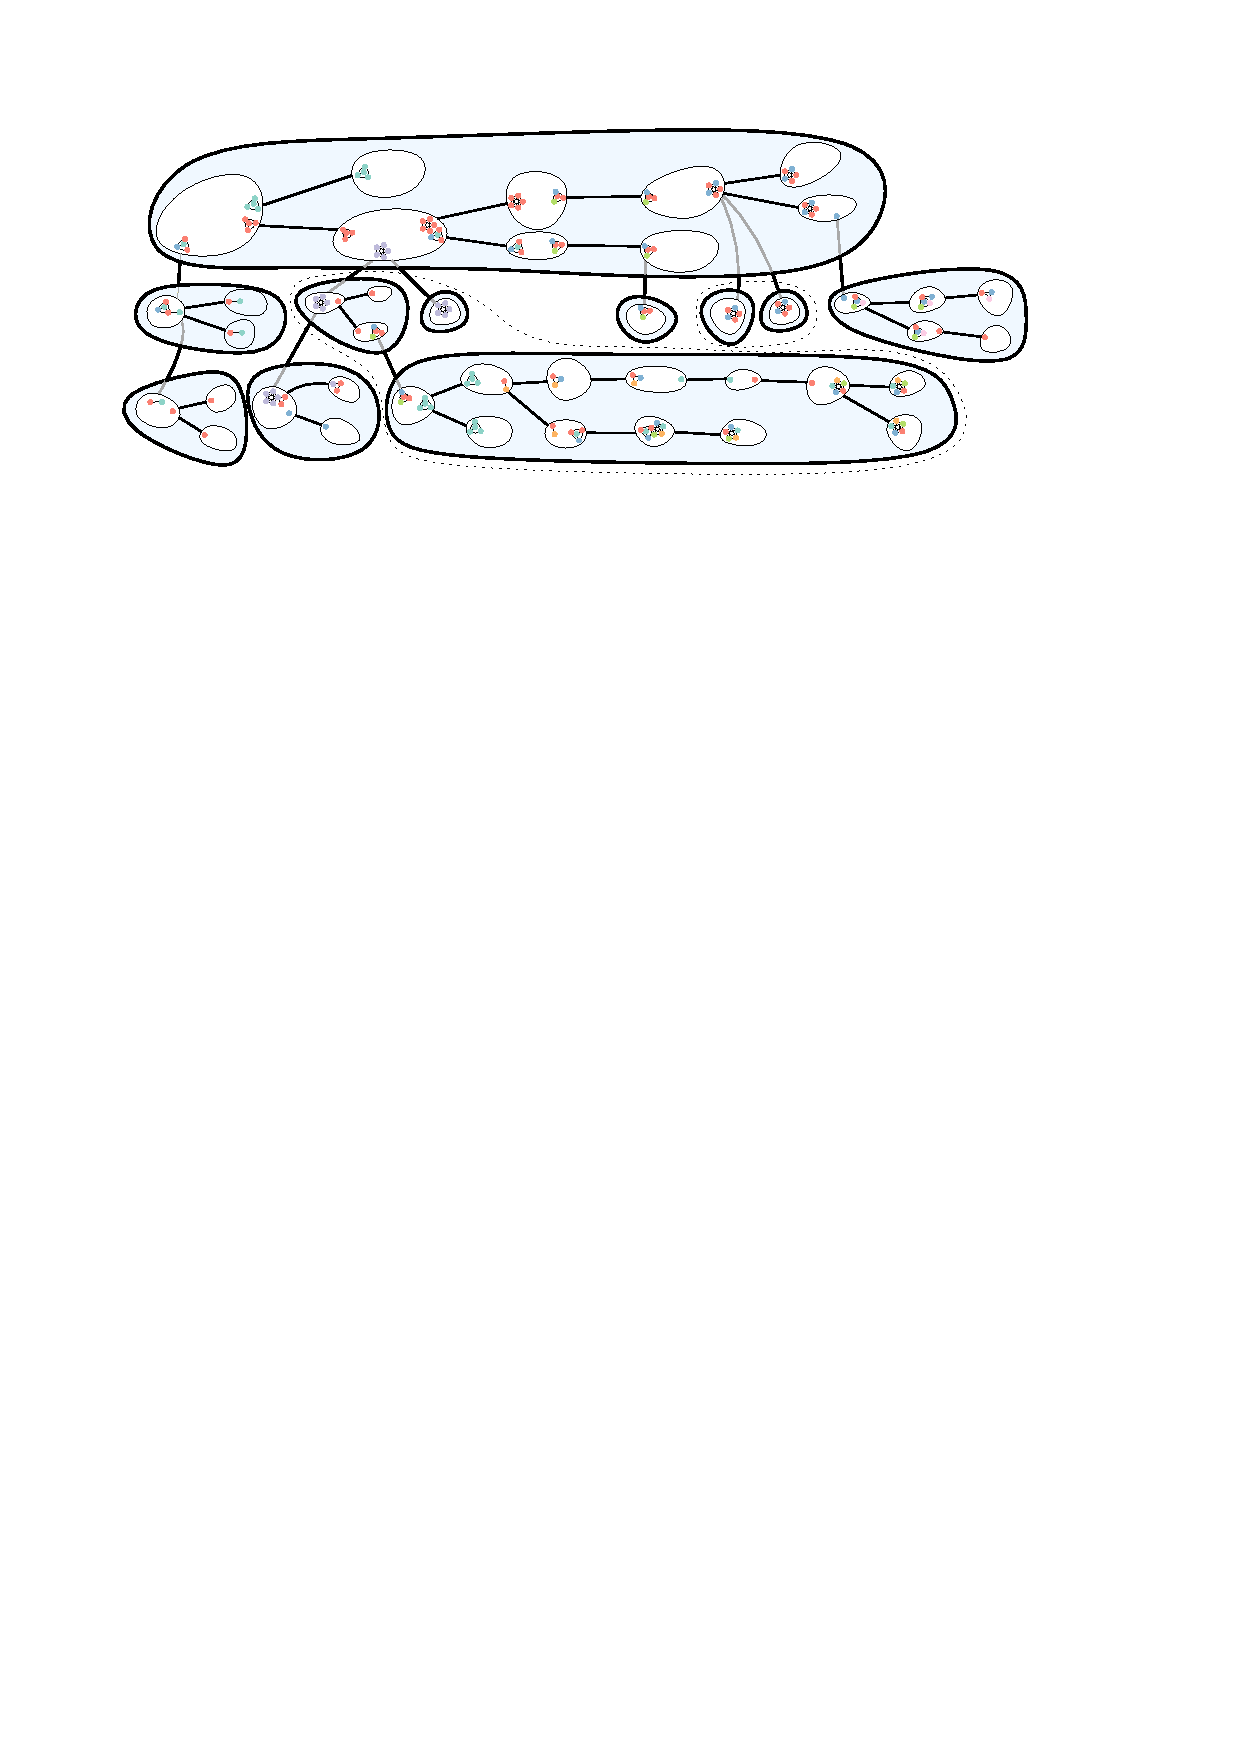
\includegraphics[page=1,width=0.95\textwidth]{figs/t_tprime.pdf} \\[-3ex]
      $\mathcal{T}$ \\[4ex]
      \includegraphics[page=2,width=0.95\textwidth]{figs/t_tprime.pdf} \\[4ex]
      \includegraphics[page=5,width=0.95\textwidth]{figs/t_tprime.pdf} \\[0ex]
      $\mathcal{T}'$
    \end{center}
    \caption{The proof of \cref{PlainRealMainTechnical} works by partitioning the tree $T$ indexing a tree-decomposition $\mathcal{T}$ (top) into skinny subtrees (middle) so that contracting these gives a short tree $T'$ indexing the tree-decomposition $\mathcal{T}'$ (bottom).}
    \label{overview_fig}
  \end{figure}

  The proof then proceeds in two steps: The first step is to show that graphs that have skinny tree-decompositions whose torsos admit efficient weighted mixed labelling schemes also have efficient weighted mixed labelling schemes (\cref{skinny_labelling}). The second shows that graphs that have tree-decompositions of sufficiently small height  whose torsos admit efficient weighted mixed labelling schemes also admit efficient weighted mixed labelling schemes (\cref{small_height}).  These are then combined to give a more precise version of \cref{PlainRealMainTechnical} that quantifies the efficiency of the resulting weighted mixed labelling scheme (\cref{RealMainTechnical}).

  The first step makes use of the fact that each skinny subtree of $T$ defines a skinny tree-decomposition which we linearize to obtain a path decomposition with adhesion-width $\Oh(bk)$. The solution of this path-decomposition-based subproblem involves a combination of techniques that have been developed for similar (though unweighted) problems \cite{gavoille.labourel:shorter,dujmovic.esperet.ea:adjacency}. The extension to the weighted version (and mixed labellings) is achieved by using alphabetic binary trees rather than the balanced binary trees used in \cite{gavoille.labourel:shorter,dujmovic.esperet.ea:adjacency}.  One critical detail  that our construction ensures and the solution makes use of, is that it guarantees more than just the adhesion-width bound \(\Oh(bk)\). In the linearization we use the fact that each vertex has at most $k$ neighbours in the parent adhesion of its home node, and this is important.

  The generalization provided by weighted mixed labelling schemes is crucial for the second step, as we now explain.
  Let $w$ be a vertex of $G$ and let $x_0,\ldots,x_s$ be the path from the root $x_0$ of the short tree $T'$ to the home node $x_s$ of $w$.  (Most of) the vertex label $\mu(w)$ is obtained by concatenating the labels $\mu_{x_0}(K_1),\ldots,\mu_{x_{s-1}}(K_s),\mu_{x_s}(w)$ where $\mu_{x_0}$ is a mixed labelling of $\torso{G}{B_{x_0}}$, $\mu_{x_i}$ is a mixed labelling of $\torso{G}{B_{x_i}}-B_{x_{i-1}}$, and $K_i$ is a clique whose vertex-set is contained in the adhesion $B_{x_{i-1}}\cap B_{x_i}$, for each $i\in\{1,\ldots,s\}$.  This serves two purposes:
  \begin{enumerate}
      \item For two vertices $v$ and $w$, the longest common prefix of $\mu(v)$ and $\mu(w)$ can be used to determine if the home nodes in $\mathcal{T}'$ for $v$ and $w$ are in an ancestor-descendant relationship (or if $v$ and $w$ have the same home node.)
      \item The vertex label $\mu(w)$ for $w$ can be augmented to explicitly store $\kappa(K_{x_i},v)$ for each neighbour $v$ of $w$ whose home node is a strict ancestor $x_{i}$ of $w$'s home node $x_{s}$. Each such vertex $v$ is necessarily contained in the adhesion $B_{x_s}\cap B_{x_{s-1}}$.  Since the adhesion-width of $\mathcal{T}'$ is at most $k$, this adds at most $k\cdot g_2(n)$ to the length of $\mu(w)$.
  \end{enumerate}
  The total length of vertex labels is controlled by using the appropriate weight function $\omega_{x}$ when computing the weighted mixed labelling for the lower torso of each node $x$ of $T'$.


  Despite the simplicity of this high-level description, getting all of this to work involves carefully managing the interplay between the skinnyness parameter $b$, the input parameters $g_1$, $g_2$, and $g_3$ of the weighted mixed labelling scheme for each torso of the original tree-decomposition $\mathcal{T}$, the parameters $g_1'$, $g_2'$ and $g_3'$ of the weighted mixed labelling scheme for graphs with skinny tree-decompositions, and the parameters $g_1''$, $g_2''$ and $g_3''$ of the weighted mixed labelling scheme for the entire graph. For example, the lengths of the labels $\mu_{x_0}(K_1),\ldots,\mu_{x_{s-1}}(K_s),\mu_{x_s}(w)$ described above form a telescoping series that sums to $\log\Omega - \log\omega(w) + s\cdot g'_3 + g'_1$, so the value of $g_1''$ is at least $s\cdot g'_3 + g'_1$, which is why we require that $T'$ is short, since the height of $T'$ upper bounds $s$.  This requires using a large value of $b$, which makes the subtrees used to define $T'$ less skinny, this increases the value of $g_2'$, which increases the length of the second part of $\mu(w)$, which has length $k\cdot g_2'(n)$.
  Optimizing the trade-off between the skinnyness parameter $b$ and the height $h$ of $T'$ ultimately yields the $\Oh((\log n)^{3/4})$ lower order term in our final bound.


  To deduce \cref{main_result} from \cref{PlainRealMainTechnical}, we use two ingredients.  The first ingredient is a rough
  version of the Robertson-Seymour Graph Minor Structure Theorem due to \citet{dujmovic.joret.ea:planar} which states that every graph in a proper-minor-closed family $\mathcal{G}$ has a tree-decomposition whose torsos have `product-plus-apex structure'. More specifically, each torso is a graph that, after the removal of at most $a(\mathcal{G})$ vertices, is a subgraph of a strong graph product $H\boxtimes P$, where $P$ is a path and the treewidth of $H$ is at most $t(\mathcal{G})$.  The second ingredient is a generalization of the adjacency labelling scheme for `product structured' graphs of \citet{dujmovic.esperet.ea:adjacency} to the weighted mixed labelling setting.  This generalization, which is discussed in \cref{weighted_product_proof}, is fairly straightforward: The notion of clique labels and membership labels is already implicit in \cite{dujmovic.esperet.ea:adjacency} and the addition of vertex weights is accomplished by a standard trick of simulating weight by multiplicity.

\subsection{Paper organization}

  The remainder of the paper is organized as follows:  \Cref{building_blocks} reviews some basic background material and establishes the relationship between the skinnyness of subtrees and the height of $T'$ discussed above.  \Cref{weighted_mixed_section} introduces weighted mixed labelling schemes and proves \cref{PlainRealMainTechnical}.  \Cref{gpmst_section} describes the Graph Minor Product Structure Theorem from \cite{dujmovic.joret.ea:planar}, the adaptation of the adjacency labelling scheme from \cite{dujmovic.esperet.ea:adjacency} to the setting of weighted mixed labellings, and puts everything together to prove \cref{main_result}. We conclude in \Cref{conclusion} by explaining how the constructive nature of \cref{main_result} leads to a
polynomial-time labelling algorithm.

  \section{Building blocks}\label{building_blocks}

Let \defin{$\N$} be the set of all nonnegative integers, and let \defin{$\N^+$} be the set of all positive integers.

  In this paper, all graphs are finite, simple, and undirected.  For a graph $G$, \defin{$V(G)$} denotes the vertex-set of $G$, \defin{$E(G)$} denotes the edge-set of $G$, and \defin{$K(G)$} denotes the set of cliques in $G$, where a \defin{clique} is a set of pairwise adjacent vertices. For standard graph theory terms, we refer the reader to the textbook by \citet{diestel:graph}.

%\piotr{define spanning subgraph.} \david{not needed in my opinion, better to reference  Distel's textbook for undefined terms}

%  \pat{TODO: Change all occurrences of $V(K)$ to $K$, since a clique is defined as a set of vertices, not a subgraph.} \david{done}


  \subsection{Trees and Forests}

  For a rooted tree $T$ with root $r\in V(T)$ and a node $x$ of $T$, define \defin{$P_T(x)$} to be the path in $T$ from $x$ to $r$.    A \defin{forest} $F$ is a graph (possibly disconnected) each whose components is a tree.  If each component of a forest $F$ is a rooted tree then, then $F$ is a \defin{rooted} forest. For a node $x$ in a rooted forest $F$ is $\mathdefin{P_F(x)}:=P_T(x)$ where $T$ is the component of $F$ that contains $x$.

  Let $F$ be a rooted forest.  For each $x\in V(F)$,
  the \defin{$F$-depth} of $x$, denoted \defin{$\depth_F(x)$}, is the number of edges in $P_T(x)$.
  The \defin{height} of $F$, denoted $\mathdefin{\height(F)}:=\max_{x\in V(F)}\height_F(x)$, is the maximum $F$-depth of a vertex in $F$.
  For each $y\in V(F)$ and each $x\in V(P_F(y))$ (including $y$),  the vertex $x$ is a \defin{$F$-ancestor} of $y$ and $y$ is a \defin{$F$-descendant} of $x$.  For each $x\in V(F)$, \defin{$F_x$} denotes the subtree of $F$ induced by all $F$-descendants of $x$.
  For each edge $xy$ of $F$ where $x$ is an $F$-ancestor of $y$, we say that $x$ is the \defin{$F$-parent} of $y$ and $y$ is a \defin{$F$-child} of $x$.
  We say that a set $S\subseteq V(F)$ is a \defin{$F$-antichain}, if there are no distinct $x,y\in S$ such that $x$ is a $F$-ancestor of $y$.  (When there is no danger of ambiguity, we may drop the leading $F$- from $F$-depth, $F$-ancestor, $F$-descendant, $F$-parent, and $F$-child.)
  We treat each subgraph $F'\subseteq F$, as a rooted forest in which each component $T$ of $F'$ is rooted at the node of $T$ having minimum $F$-depth.  For each $i\in\N^+$, the \defin{$i$-th layer} of $F$ is $\mathdefin{L_i(F)}:=\{x\in V(F):\depth_F(x)=i-1\}$.
  Thus, $L_1(F)$ is the set of roots of components of $F$.

  For a rooted tree $T$ and any set $S\subseteq V(T)$, the \defin{lowest common $T$-ancestor} of $S$, denoted \defin{$\lca_T(S)$}, is the node in $\bigcap_{x\in S} V(P_T(x))$ of maximum $T$-depth.



  \subsection{Tree-Decompositions and Forest-Decompositions}




  % We will often take subgraphs of a graph $G$ defined by subtrees of a tree indexing a tree-decomposition of $G$.  When we do this, we will  (implicitly) make use of the following fact: If a rooted tree-decomposition $\calT=(T,(B_x \mid x\in V(T)))$ is downward-normalised and upmost then, for any node $x$ of $T$ and any $T$-child $y$ of $x$, the tree-decomposition $\mathcal{T}_y:=(T_y,(B_z\setminus B_x\mid z\in V(T_y)))$ is a downward-normalised upmost tree-decomposition of the graph $G_y:=G[\bigcup_{z\in V(T_y)} B_z]-B_x$.   Furthermore, $B_v\cap B_w\neq\emptyset$ for each edge $vw$ of $T$, then $B_v\cap B_w\setminus B_z\neq\emptyset$ for each edge $vw$ of $T_y$. In words, if every edge of $T$ defines an non-empty adhesion in $\mathcal{T}$, then every edge of $T_y$ defines a non-empty adhesion in $\mathcal{T}_y$.
  % Throughout the rest of this paper, we will implicitly assume that any rooted tree-decomposition we are considering is downward-normalised and upmost.
  Let $G$ be a graph and $\calT=(T,(B_x \mid x\in V(T)))$ be a tree-decomposition of $G$. If $T$ is a path, then $\calT$ is a \defin{path-decomposition} of $G$, simply denoted by the sequence $(W_1, W_2, \dots, W_m)$ of the bags in the order of the vertices in the underlying path.

  It will be convenient to work with forest-decompositions, which are the natural generalization of a tree-decomposition that allow the graph indexing the bags to be a forest.  Specifically, $(F,(B_x\mid x\in V(F))$ is a \defin{forest-decomposition} of a graph $G$ if $F$ is a forest, for each edge $vw$ of $G$ there exists $x\in V(F)$ with $v,w\in B_x$, and for each vertex $v$ of $G$, $F[\{x\in V(F)\mid v\in B_x\}]$ is connected.  A forest-decomposition $(F,(B_x\mid x\in V(F))$ of a graph $G$ is \defin{tidy} if
  \begin{enumerate*}[label=(\arabic*)]
  \item $B_x\neq\emptyset$ for each $x\in V(F)$,
  \item $B_y\not\subseteq B_x$ for each $y\in V(F)$ with an $F$-parent $x$;
  \item $B_z \cap B_y \not\subseteq B_y\cap B_x$ for each $z\in V(F)$ with an $F$-parent $y$ and an $F$-grandparent $x$.
  \end{enumerate*}


  % Since we can always remove any vertex or edge of $F$ that violates the tidy condition, we have the following observation, which allows us to focus on tidy forest-decompositions.

\piotr{$G$ needs to have at least one vertex.}
  \begin{obs}\label{tidy_forest}
    Let $G$ be a graph and let $(F,(B_x\mid x\in V(F)))$ be a forest-decomposition of $G$.  Then there exists $F'\subseteq F$ such that $(F',(B_x\mid x\in V(F')))$ is a tidy forest-decomposition of $G$.
  \end{obs}
  We make use of the fact that tidy forest decompositions remain tidy when we remove the root bags and their contents.  More precisely, let $\mathcal{F}:=(F,(B_x\mid x\in V(F)))$ be a tidy forest decomposition of a graph $G$, let $R$ be the set of roots in $F$, let $B_R:=\bigcup_{r\in R}B_r$, and let $C_x:=B_x\setminus B_R$ for each $x\in V(F)$.  Then $(F-R,(C_x\mid x\in V(F-R)))$ is a tidy rooted forest decomposition of $G-B_R$.


  % , then $(F-R,(B_x\$

  % \pat{Come back and put this into the tidy definition.}
  % A forest-decomposition $\calT=(F,(B_x \mid x\in V(F)))$ is \defin{normalised} if $B_x\not\subseteq B_y$ for every two distinct nodes $x,y\in V(T)$.   Any forest-decomposition $\mathcal{F}$ can be normalised through a sequence of edge contractions and bag mergers to produce a normalised tree-decomposition $\mathcal{F}'$ whose width and adhesion-width are not greater than the width and adhesion-width of $\mathcal{F}$, respectively. Furthermore, every torso of $\mathcal{F}'$ is also a torso of $\mathcal{F}$.  A rooted forest-decomposition $\mathcal{F}=(F,(B_x \mid x\in V(F)))$ is \defin{downward-normalised} if each root $r$ of $F$ has a non-empty bag $B_r$ and, for each node $y$ of $T$ and each $T$-ancestor $x\neq y$ of $y$, $B_y\not\subseteq B_x$.  Clearly, if $\mathcal{T}$ is normalised then it is also downward-normalised for any choice of root $r\in V(T)$.  A rooted forest-decomposition $\calT=(T,(B_x \mid x\in V(T)))$ is \defin{upmost} if, for each adhesion $A$ of $\calT$, there exists a node $x$ of $T$ such that, for any edge $yz$ of $T$ with $B_y\cap B_z\subseteq A$, $x\in\{z,y\}$ and the node in $\{z,y\}\setminus\{x\}$ is a $T$-child of $x$.  Any downward-normalised rooted tree-decomposition $\calT=(T,(B_x \mid x\in V(T)))$ of a graph $G$ can be made upmost by swapping edges in $T$
  % % \gwen{I'm not sure what swapping edges means here, moving edges? in any case I agree it works} \pat{In general, replacing, in particularly moving the upper endpoint of an edge up to the parent (repeatedly)} \gwen{ok}
  % to obtain a tree $T'$ such that $\mathcal{T}':=(T', (B_x \mid x\in V(T')))$ is a tree-decomposition of $G$, each adhesion in $\mathcal{T}'$ is an adhesion in $\mathcal{T}$ and each torso in $\mathcal{T}'$ is a subgraph of a torso in $\mathcal{T}$.








  \subsection{Weight Functions}

  For a non-empty set $S$, a \defin{weight function} over $S$ is a mapping $\omega:S\to\R^+$ of the elements of $S$ onto positive real numbers.  When $X$ is a subset of $S$, we use the shorthand $\mathdefin{\omega(X)}:=\sum_{x\in S}\omega(x)$.  When $S:=V(G)$ is the vertex-set of a graph $G$ and $H$ is a subgraph of $G$, we use the shorthand $\mathdefin{\omega(H)}:=\omega(V(H))$.

  Let $\omega:S\to\R^+$ be a weight function.  For each $x\in S$, the \defin{(Kraft) ideal codeword length} for $x$ is $\log\omega(S)-\log\omega(x)$.
  It will be convenient to place some upper bound on the Kraft ideal codeword length or, equivalently, on the ratio of total weight, $\omega(S)$ to minimum weight $\min_{x\in S}(\omega(x))$.  The following observation gives a way to do this without increasing the ideal codeword length of each $x\in S$ by more than $1$:

  \begin{obs}\label{obs:nice}
    For every weight function $\omega:S\to\R^+$, there exists a weight function $\omega'(S)\to\N^+$ such that $\log\omega'(S)-\log\omega'(x)\le\min\{\log|S|,\;\log\omega(S)-\log\omega(x)\}+2$, for each $x\in S$.
  \end{obs}

  \begin{proof}
    By dividing every weight by $\min_{x\in S}\omega(x)$ we may assume, without loss of generality, that $\omega(x)\ge 1$ for each $x\in S$, since this does not change the value of the right-hand side in the inequality.
    For each $x\in S$, define $\omega'(x):=\ceil{\max\{\omega(S)/|S|,\; \omega(x)\}}$.  Then $\omega'(S)<\sum_{x\in S}(\omega(S)/|S|+\omega(x)+1)= 2\omega(S)+|S|\le 3\omega(S)$.  For each $x\in S$, the inequality $\omega'(x)\ge \omega(x)$ implies that $\log\omega'(S)-\log\omega'(x)\le\log \omega(S)-\log\omega(x)+\log 3$ and the inequality $\omega'(x)\ge \omega(S)/|S|$ implies that $\log\omega'(S)-\log\omega'(x)\le \log\omega(S)-\log(\omega(S)/|S|) + \log 3 = \log|S| + \log 3$.
  \end{proof}

  % We will normally apply \cref{obs:nice} in passing at the beginning of proofs where $S=V(G)$ for some $n$-vertex graph $G$.  This will allow us to assume that the maximum ideal codeword length is \gwen{at most?} $\log n + 1$.

  Tidy rooted forest-decompositions define a useful weight function over the nodes of their indexing forests.
  Let $G$ be a graph and let $\mathcal{F}:=(F,(B_x \mid x\in V(F)))$ be a tidy rooted forest-decomposition of $G$.
    We define a weight function $\omega_\mathcal{T}:V(T)\to \N^+$ as follows.
      For each node $x$ of $T$, we define
  \[
      \mathdefin{\omega_{\mathcal{T}}(x)}=\begin{cases}
      |B_x|&\textrm{if $x$ is the root of $T$,}\\
      |B_x\setminus B_y|&\textrm{if $x$ is not the root of $T$ and $y$ is the $T$-parent of $x$.}
      \end{cases}
  \]
  Note that $\sum_{x\in V(T)}\omega_\mathcal{T}(x)=|V(G)|$.    \pat{Be careful how we use this.  I feel like we've used it later to mean $\omega_{\mathcal{F}}(x)=\sum_{v\in B_x\setminus A} \omega(v)$....}
  % \pat{This is ok, but in the rest, I've been using the convention that $x$ is a parent of $y$ and $z$ is a descendant of $y$. This happens in a few places, so I think it's helpful to keep it consistent.}

  \subsection{Shannon and Shannon--Fano--Elias Codes}

  A \defin{code} for a set $S$ is an injective function $\lambda:S\to\{0,1\}^*$ that maps each element in $S$ to a distinct binary string.  A code is \defin{prefix-free} if $\lambda(x)$ is not a prefix of $\lambda(y)$ for all distinct $x,y\in S$.
  % We make use of the following fundamental result by Shannon.

  % \begin{lem}[\citep{shannon:mathematical,shannon:mathematical2}]
  % \label{shannon_code}
  %   Let $S$ be a non-empty set and let $\omega:S\to\R^+$.  Then there exists a prefix-free code $\pi:S\to\{0,1\}^*$ such that $|\pi(x)|\le \log\omega(S)-\log\omega(x)+1$ for each $x\in S$.
  % \end{lem}

  A rooted tree $T$ is a \defin{binary tree} if each node of $T$ has at most two children among which at most one is the \defin{left child} and at most one is the \defin{right child}.
  A binary tree $T$ is \defin{full} if for every node $x$ of $T$,
  either $x$ has two children or $x$ has no children.
  A full binary tree $T$ is \defin{complete} if all the leaves of $T$ have the same depth in $T$.
  Let $T$ be a binary tree. There is a natural ordering, called \defin{left-to-right ordering}, of the leaves of $T$, such that for every node $x$, if $x$ has two children then all the leaf descendants of the left child of $x$ precede all the leaf descendants of the right child of $x$.


  The following result is a variant of Alphabetic Binary Trees. Similar results (with the constant $3$ replaced by $2$) are well-known and there are several proofs \cite{knuth:art_iii,mehlhorn:nearly,gilbert.moore:variable_length}. We provide a proof of the weaker statement here because it illustrates a simple but powerful technique---\defin{simulating weight by multiplicity}---that we will use again later.

   \begin{lem}\label{shannon_fano_elias_tree}\label{shannon_fano_elias}
    Let $S$ be a linearly ordered set and let $\omega:S\to\N^+$. Then there exists a binary tree $T$ such that $S$ is the set of leaves of $T$,
    the linear order on $S$ agrees with the left-to-right-order of the leaves in $T$, and for each $x\in S$
    \[
    \depth_{T}(x)\le \log\omega(S) - \log\omega(x) + 3.
    \]
  \end{lem}

% \piotr{I rewrote this proof.} \pat{Looks good.}

   \begin{proof}
     Let $h:=\lceil\log\omega(S)\rceil$.
     Let $Q$ be the complete binary tree of height $h$, so with $2^h$ leaves.
     %, by repeatedly removing a leaf of $Q$ until $Q$ has exactly $\omega(S)$ leaves.
     For each $x\in S$, define the $\omega(x)$-element set
     \[  S_{\omega}(x):=\set{(x,1),\,(x,2),\,\ldots\,,\,(x,\omega(x))}\]
     and let $S_\omega:=\bigcup_{x\in S}S_{\omega}(x)$.  Then $|S_\omega|=\omega(S)$.  Treat $S_{\omega}$ as a linearly ordered set by using lexicographic order and rename the leftmost $\omega(S)$ leaves of $Q$, in order, with elements of $S_{\omega}$.

    Now for each $x\in S$, we are going to fix a node $r(x)$ in $Q$ such that
    (1) all the leaves of $Q_{r(x)}$ lie in $S_{\omega}(x)$; and
    (2) $Q_{r(x)}$ contains at least $\omega(x)/4$ leaves.

     Let $x\in S$.
     If $\omega(x)=1$ then define $r(x):=(x,1)$, which is a leaf of $Q$.
     Clearly, (1) and (2) holds.
     Now suppose that $\omega(x)\geq2$.
     Consider the lowest common $Q$-ancestor $y$ of $S_{\omega}(x)$.
     Thus, $y$ is an internal node of $Q$ and
     both children of $y$ contain in their subtree a leaf in $S_{\omega}(x)$.
     Since $S_{\omega}(x)$ is a set of consecutive leaves in $Q$,
     all leaves of the left child $y'$ of $y$ in $Q$ that are in $S_{\omega}(x)$ are rightmost in $Q_{y'}$ and
     all leaves of the right child $y''$ of $y$ in $Q$ that are in $S_{\omega}(x)$ are leftmost in $Q_{y''}$.
     Let $z$ be the child of $y$ in $Q$ such that $Q_z$ has at least $\omega(x)/2$ leaves in $S_{\omega}(x)$ and let $S_z$ be the set of all such leaves.
     Thus, $|S_z|\geq \omega(x)/2$.
     Since the argument is completely symmetric in these cases, assume that $z$ is the left child of $y$.
     Consider a path in $Q_z$ starting from $z$ and always taking an edge to the right child of the current node until we finish at a leave.
     Let $v$ be the first vertex of that path such that $Q_v$ has all leaves in $S_z$.
     If $v=z$ then we set $r(x):=v$. Clearly (1) and (2) holds.
     Suppose that $v\neq z$.
     Let $u$ be the parent of $v$.
     Since the set of leaves of $Q_u$ form an interval of rightmost leaves of $Q_z$ and since $Q_u$ contains a leaf not in $S_z$, we conclude that $Q_u$ contains all nodes in $S_z$ as leaves.
     Therefore, $Q_v$ contains at least $|S_z|/2$ vertices of $S_z$ as leaves.
     We set $r(x):=v$ and again (1) and (2) holds.

     Note that the set $\set{r(x) \mid x\in S}$ is a $Q$-antichain.
     Indeed, if $x,y\in S$, $x\neq y$ and $r(x)$ is a $Q$-ancestor of  $r(y)$, then the leaves of $Q_{r(y)}$ are contained in the leaves of $Q_{r(x)}$ which by (1) implies that $Q_{r(x)}$ contains all nodes in $S_{\omega}(y)$ as leaves.
     However, again by (1) all the leaves of $Q_{r(x)}$ lie in $S_{\omega}(x)$ which is disjoint from $S_{\omega}(y)$, a contradiction.

    Let $x\in S$. Since $Q_{r(x)}$ contains at least $\omega(x)/4$ leaves, we have that
$\height(T_{r(x)}) \geq \log(\omega(x)/4) = \log\omega(x) - 2$.
Finally,
     \begin{align*}
     \depth_Q(r(x))
     &\le \height(Q)-\height(Q_{r(x)})\\
     &\le \lceil\log\omega(S)\rceil - (\log\omega(x) - 2)\\
     &\le \log\omega(S) - \log\omega(x) +3.
     \end{align*}

    Let $T:=\bigcup_{x\in S} P_Q(r(x))$.
    Since $\set{r(x) \mid x\in S}$ is a $Q$-antichain,
    we conclude that $\set{r(x)\mid x\in S}$ is the set of all leaves of $T$.
    Identifying each leaf $r_x$ of $T$ with $x$ for each $x\in S$ gives the desired tree.
   \end{proof}


  %  The same proof that derives \cref{shannon_code_bounded} from \cref{shannon_code} can be used to derive the following corollary of \cref{shannon_fano_elias_tree}.
  %  \begin{cor}\label{shannon_fano_elias_tree_bounded}\label{shannon_fano_elias_bounded}
  %   Let $S$ be a linearly ordered set and let $\omega:S\to\N^+$. Then there exists a binary tree $T$ of height at most $\log|S|+4$ such that $S$ is the set of leaves of $T$,
  %   the linear order on $S$ agrees with the left-to-right-order of the leaves in $T$, and for each $x\in S$
  %   \[
  %   \depth_{T}(x)\le \log\omega(S) - \log\omega(x) + 4.
  %   \]
  % \end{cor}


  In coding theory, \cref{shannon_fano_elias} is the basis of the Shannon-Fano-Elias coding scheme, as we now explain.  By assigning each edge $e$ of a binary tree $T$ a $0$ or $1$ depending on whether $e$ joins a parent to its left or right child, we obtain an encoding of each root-to-leaf path in $T$ as a binary string. Doing this with the tree from \cref{shannon_fano_elias_tree}, we obtain the following.

  \begin{cor}\label{shannon_fano_elias_code}\label{shannon_fano_elias_cor}
    Let $S$ be a linearly ordered set and let $\omega:S\to\N^+$.  Then there exists a code $\rho:S\to \{0,1\}^\star$ for $S$ such that:
    \begin{enumerate}[nosep,nolistsep,label=(\alph*)]
      \item $|\rho(x)|\le \log\omega(S) - \log\omega(x)+3$ for each $x\in S$, and
      \item $\rho(x)$ is lexicographically less than $\rho(y)$ for each $x,y\in S$ with $x< y$ in $S$.
    \end{enumerate}
  \end{cor}



  \subsection{On Multipart Labels}
  \label{multipart}

  In many case, a label (a bitstring) will have a variable number of parts (also bitstrings), of varying lengths.  We write this as $s:=\langle s_1,\ldots,s_p\rangle$, where each of $s_1,\ldots,s_p$ is a (possibly empty) bitstring.  The concatenation of $s_1,\ldots,s_p$, has length
  \[
     \textstyle |s|=|s_1,\ldots,s_p|=\sum_{i=1}^p|s_p| \enspace .
  \]
  This ignores the important issue that, in order for a decoder to extract the individual parts $s_1,\ldots,s_p$ it must know the number of parts, $p$, and (at least $p-1$ of) the lengths $|s_1|,\ldots,|s_p|$.  We handle this by encoding the value of $p$ and the lengths $|s_1|,\ldots,|s_{p}|$ and prepending these to $s$. This is most easily done using Elias's code $\gamma:\N^+\to\{0,1\}^*$ for positive integers, in which each $x\in\N^+$ is encoded by a self-delimiting binary string $\gamma(x)$ with $|\gamma(x)|\le 2\lfloor \log x  \rfloor  + 1$ \cite{elias:universal}.\footnote{For each $x\in\N^+$, $\gamma(x)$ consists of $\lfloor\log x\rfloor$ 0 bits, followed by the binary representation of $x$ (which begins with a $1$ bit and has length $\lfloor\log x\rfloor+1$).} In our application $s_i$ may have zero length and $p$ may even be equal to zero, so that that codeword for each $x\in\N$ is $\gamma(x+1)$ and has length $2\floor{\log (x+1)}+1$.
  In this way, we obtain a self-delimiting encoding of $s_1,\ldots,s_p$ as
  \[  \mathdefin{\langle s_1,\ldots,s_p\rangle}:=\gamma(p+1),\gamma(|s_1|+1),\ldots,\gamma(|s_p|+1),s_1,\ldots,s_p \enspace ,
  \]
  which has length
  \begin{equation}
    |\langle s_1,\ldots,s_p\rangle| = \textstyle\sum_{i=1}^p|s_i|+\Oh(\lgg p) + \Oh(\sum_{i=1}^p\lgg|s_i|) \enspace , \label{encoding_cost}
  \end{equation}
  where $\mathdefin{\lgg x} := \log\max\{2,x\}$ (just so that $\lgg(x)$ is defined and $\lgg(x)\ge 1$ for each $x\in\N$).    The bits of $\langle s_1,\ldots,s_p\rangle$ that come from $s_1,\ldots,s_p$ are called the \defin{payload} bits and the remaining bits are called the \defin{bookkeeping} bits of $\langle s_1,\ldots,s_p\rangle$.
  In our setting it will always be the case that $p\in o(\log n)$ and we will use \cref{obs:nice} to ensure that $|s_i|\in \Oh(\log n)$ for each $i\in[p]$.
  Thus, the number of bookkeeping bits in $\langle s_1,\ldots,s_p\rangle$  is $\Oh(p\log\log n)$.

  \pat{TODO: Push the $\langle s_1,\ldots,s_p\rangle$ notation to other sections.}

  \subsection{Separators with Low Pathwidth and Low Path-Adhesion-Width}

  For an integer $b\in\N^+$,
  a rooted tree $T$ is \defin{$b$-skinny},
  if $|L_i(T)|\le b$ for each $i\in\N^+$.  A rooted tree-decomposition $(T,(B_x\mid x\in V(T)))$ of a graph $G$ is \defin{$b$-skinny} if $T$ is $b$-skinny.  The following lemma shows how to construct a $(1/b)$-separator using the bags in a $b$-skinny subtree of a tree-decomposition.


  \begin{lem}\label{low_pathwidth_separator}
    Let $b>1$, let $T$ be a rooted tree, let $\omega:V(T)\to\R^+$, and let
    \[
    X:=\set{x\in V(T)\mid\omega(T_x)>\omega(T)/b}.
    \]
    Then:
    \begin{enumerate}[nosep,nolistsep,label=(\alph*)]
      \item\label{connected} $T[X]$ is connected and contains the root of $T$;
      \item\label{skinny} $|X\cap L_i(T)|< b$, for each $i\in\N^+$; and
      \item\label{light} $\omega(C)\le \omega(T)/b$ for each component $C$ of $T-X$.
    \end{enumerate}
  \end{lem}

  \begin{proof}
    Let $r$ be the root of $T$.  Since $b>1$, we have $\omega(T_r)=\omega(T)>\omega(T)/b$. % so $r\in X$.
    For $x\in X\setminus\{r\}$, let $y$ be the $T$-parent of $x$, then
    $\omega(T_y)\ge \omega(y)+\omega(T_x)>\omega(T_x)>\omega(T)/b$.
    %so $y\in X$.
    Therefore $r\in X$ and, for each $x\in X\setminus\{r\}$, $X$ contains the $T$-parent of $x$. Thus $T[X]$ is connected.
    This proves~\ref{connected}.

    For each $i\in\N^+$, the subtrees in $\set{T_x \mid x\in X\cap L_i(T)}$ are pairwise vertex-disjoint, so
    \[
    \omega(T) \ge \sum_{x\in X\cap L_i(T)} \omega(T_x)> \sum_{x\in X\cap L_i(T)}\omega(T)/b = |X\cap L_i(T)|\cdot\omega(T)/b.
    \]
    Rewriting this inequality gives $|X\cap L_i(T)|<b$ for each $i\in\N^+$.
    This proves~\ref{skinny}.

    By~\ref{connected}, each component $C$ of $T-X$ is a subtree of $T$ that is rooted at some node $y$ whose $T$-parent is in $X$.  Since  $y\not\in X$, $\omega(C)=\omega(T_y)\le \omega(T)/b$.
    This proves~\ref{light}.
  \end{proof}


  \pat{This needs to be adjusted to accept a forest decomposition, or we should have a corollary about forest decompositions.}
  \begin{cor}\label{b_skinny_decomp}
    For every $b>1$, every $n\in\N^+$, every $n$-vertex graph $G$ and every tree-decomposition $\mathcal{T}:=(T,(B_x\mid x\in V(T)))$ of $G$, there exists a tree-decomposition $\mathcal{Q}:=(Q,(D_x\mid x\in V(Q)))$ of $G$ such that
    % \piotr{Actually, we have a number of tree decompositions here. I suggest to replace $\torso{G}{D_x}$ with $G\langle\mathcal{Q},x\rangle$}
    \begin{enumerate}[nosep,nolistsep,label=(\alph*)]
      \item\label{prop_adhesion}
      each adhesion of $\mathcal{Q}$ is an adhesion of $\mathcal{T}$;
      \item\label{prop_skinny_torso} for each $q\in V(Q)$, $\torso{G}{D_q}$ has a $b$-skinny tree-decomposition $(T(q), (B_y\mid y\in V(T(q))))$ where $T(q)$ is a subtree of $T$; and
      \item\label{prop_geometric} \sout{for each $q\in V(Q)$, $\omega_\mathcal{Q}(Q_{q})\le n/b^{\depth_{Q}(q)}$.}
    \item\piotr{I suggest an item replacing the one one above: $\height(Q) \leq \log_{b} n$}
    \end{enumerate}
  \end{cor}

  \begin{proof}
    Fix $b>1$.
    The proof is an induction on $n$.
    To make the induction work we require additionally that
    \begin{enumerate}[nosep,nolistsep,label=(\alph*)]
    \setcounter{enumi}{3}
    \item\label{prop_extra_item} $B_r \subseteq D_s$ where $s$ is the root of $Q$.
    \end{enumerate}
    Let $G$ be an $n$-vertex graph, let $\mathcal{T}:=(T,(B_x\mid x\in V(T)))$ be a rooted tree-decomposition of $G$, and let $r$ be the root of $T$.

If $n\le b$, let $Q$ be a $1$-node tree and let $s$ be the only node which is also the root.
Let $D_s:=\bigcup_{y\in X} B_y$ and let $\mathcal{Q}:=(Q,(D_q)_{q\in V(Q)})$.
Then $\mathcal{Q}$ is a tree-decomposition with no adhesions, so~\ref{prop_adhesion} holds vacuously.
Since $\torso{G}{D_s}=G$, we can take $T(s)=T$ and then $(T(s),(B_y\mid y\in V(T(s))))$ is a $b$-skinny tree decomposition of $\torso{G}{D_s}$,
so~\ref{prop_skinny_torso} holds.
Since $V(Q)=\set{s}$ and $\depth_Q(s)=0$, \ref{prop_skinny_torso}  holds.
Also by construction~\ref{prop_extra_item} holds.

    Now assume $n> b$.
    Let $X:=\set{x\in V(T)\mid  \omega_\mathcal{T}(T_x)>n/b}$.
    By \cref{low_pathwidth_separator}, $T[X]$ is a $b$-skinny subtree of $T$ that includes $r$.
    By \cref{low_pathwidth_separator}, for each $y\in N_T(X)$ the subtree $T_y$ has weigth $\omega_\mathcal{T}(T_y)=|V(G_y)|\le n/b$. For each $y\in N_T(X)$, apply the inductive hypothesis to subgraph $G_y:=G[\bigcup_{z\in V(T_y)} B_z]$ with tree-decomposition $\mathcal{T}_y:=(T_y, (B_x\mid x\in V(T_y)))$ to obtain a tree-decomposition $\mathcal{Q}_{y}:=(Q_y,(D_x \mid x\in V(Q_y)))$ whose root bag contains $B_y$.
    Construct a tree $Q$ as follows.
    Start with a single vertex $s$ that will be the root of $Q$ and set $D_s:=\bigcup_{x\in X} B_x$.
    For each $y\in N_T(X)$, attach $Q_y$ to $Q$ by adding an edge joining the root of $Q_y$ to $s$.
    This gives the desired tree $Q$ and the desired tree-decomposition $\mathcal{Q}=(Q,(D_y:y\in V(Q)))$.

    For each $y\in N_T(X)$, each adhesion of $\mathcal{T}_y$ is an adhesion of $\mathcal{T}$.
    Thus, $\mathcal{Q}$ satisfies \ref{prop_adhesion} because each adhesion $A$ of $\mathcal{Q}$ is either an adhesion of $\mathcal{Q}_y$ or a $A=D_s\cap D_{q}$ for some $Q$-child $q$ of $s$.  In the former case, $A$ is an adhesion of $\mathcal{T}_y$, by the inductive hypothesis. In the latter case $A=B_x\cap B_y$ for some $x\in X$ and some $y\in N_T(x)$.



    % .......$(T_y, (B_x\mid x\in V(T_y))$ is a tree decomposition of $Gevery adhesion of $\mathcal{Q}_y$ is an adhesion of


    All that remains is to show that each $q\in V(Q)$ satisfies \ref{prop_geometric}.  It is clear that $q=s$ satisfies \ref{prop_geometric} since $\depth_Q(s)=0$.  Now consider some $q\in V(Q)\setminus\{s\}$.  Let $t$ be the $Q$-ancestor of $q$ with $\depth_{Q}(t)=1$ (so $t$ is a $Q$-child of $s$). By \cref{low_pathwidth_separator}, $\omega_{\mathcal{Q}}(Q_{t})\le n/b$. By the inductive hypothesis:
    \[
       \omega_{\mathcal{Q}}(Q_{q})
       \le  \omega_{\mathcal{Q}}(Q_{t})/b^{\depth_{Q_{t}}(q)}
       \le n/b^{\depth_{Q_{t}}(q)+1} = n/b^{\depth_{Q}(q)} \enspace . \qedhere
    \]
  \end{proof}



  \section{Weighted Mixed Labelling Schemes -- Proof of \cref{PlainRealMainTechnical}}
  \label{weighted_mixed_section}

We now describe the generalization of adjacency labelling schemes that we use to prove \cref{PlainRealMainTechnical}.  In the following, one can think of the graph $G^+$ as a torso $\torso{H}{B_x}$ in a tree-decomposition $\mathcal{T}$ of a larger graph $H$, the graph $G$ as an induced subgraph $H[B_x]$, and the cliques in $\mathcal{K}$ as adhesions in $\mathcal{T}$.


Let $\mathcal{G}$ be a class of graphs.
Let $g_i:\N\to\R^+$ for each $i\in[3]$.
The class  $\mathcal{G}$ admits a \defin{weighted $(g_1,g_2,g_3)$ mixed labelling scheme} of $\mathcal{G}$ if there exists a pair $(A,M)$ with
\begin{itemize}[nosep,nolistsep]
     \item $A:(\{0,1\}^*)^2\to\{0,1\}$ (the \defin{adjacency tester}); and
     \item $M:(\{0,1\}^*)^3\to\{0,1\}$ (the \defin{identity tester})
\end{itemize}
such that
for every natural $n\in\N$,
every $n$-vertex graph $G^+$ in $\mathcal{G}$,
every spanning subgraph $G$ of $G^+$,
\piotr{Can't we just work on the set of all cliques in $G^+$?}
every set of non-empty cliques $\mathcal{K}$ in $K(G^+)$, and
every weight function $\omega:V(G)\to \R^+$,
there exists an injective function $\mu: V(G)\cup \mathcal{K} \to \set{0,1}^*$ and a function $\kappa:\{(K, u)\mid K\in \mathcal{K}, u\in K\}\to \set{0,1}^*$
such that
\begin{enumerate}[nosep,nolistsep,label=(\roman*)]
    \item for all $u,v\in V(G)$
    \[
    \textrm{$A(\mu(u),\mu(v))=1$ if and only if $uv\in E(G)$;}
    \]
    \item for all $K\in \mathcal{K}$, $u\in K$, $v\in V(G)$
    \[
    \textrm{$M(\mu(K),\kappa(K, u),\mu(v))=1$ if and only if $u=v$;}
    \]
    \item for every $v\in V(G)$
    \[
    |\mu(v)| \leq \log \omega(G) - \log\omega(v) + g_1(n);
    \]
    \item for every $K\in \mathcal{K}$
    \[
    |\mu(K)|\le \log \omega(G) - \log\min_{v\in K}(\omega(v)) + g_3(n);
    \]
    \item  for every $K\in \mathcal{K}$ and $u\in K$
    \[
    |\kappa(K, u)| \leq g_2(n).
    \]
\end{enumerate}
\piotr{I changed the wording here. This needs to be propagated in proofs.}
Given $\mu$ and $\kappa$  as above we say that $(\mu,\kappa)$ is the \defin{mixed labelling} of $(G^+,G,\mathcal{K},\omega)$ for $(A,M)$.
%Given $\mu$ and $\kappa$  as above we say that $\mu$ is the \defin{mixed labelling} of $(G^+,G,\mathcal{K},\omega)$ for $(A,M)$ and $\kappa$ is the \defin{local identifier} of $(G^+,G,\mathcal{K},\omega)$ for $(A,M)$.

In the proofs, it will be convenient to consider a slightly weaker notion of weighted $(g_1,g_2,g_3)$ mixed labelling schemes.
A weight function $\omega:S\to \N^+$ is \defin{nice} if
\[
\log \omega(S) - \log \omega(x) \leq \log |S| + 2
\]
holds for every $x\in S$.
(Let us emphasize that weights are required to be positive integers here, which will be important later on.)
We then say that a class of graphs $\mathcal{G}$ admits a \defin{weak weighted $(g_1,g_2,g_3)$ mixed labelling scheme} if $\mathcal{G}$ satisfies the definition given above for weighted $(g_1,g_2,g_3)$ mixed labelling schemes, with the exception that only nice weight functions $\omega$ are considered.
The two notions are essentially equivalent, as shown by the following lemma. This will allow us to only consider nice weight functions in the proofs.

\begin{lem}
    \label{lem:nice_weights}
    Let $\mathcal{G}$ be a class of graphs.
    Let $g_i:\N\to\R$ be functions for each $i\in[3]$.
    If $\mathcal{G}$ admits a weak weighted $(g_1,g_2,g_3)$ mixed labelling scheme, then $\mathcal{G}$ admits a weighted $(g_1+2,g_2,g_3+2)$ mixed labelling scheme. %\pat{Are we ok with the abuse of notation $g_1+2$?} \piotr{Yes.}
\end{lem}
\begin{proof}
    Suppose that $\mathcal{G}$ admits a weak weighted $(g_1,g_2,g_3)$ mixed labelling scheme.
    Let $A$ and $M$ be the corresponding adjacency and identity tester, respectively.
    We will use the same pair $(A, M)$ for our weighted $(g_1+2,g_2,g_3+2)$ mixed labelling scheme.
    Let $n\in \N$, let $G^+$ be a  $n$-vertex graph  in $\mathcal{G}$, let $G$ be a spanning subgraph $G$, let $\mathcal{K}$ be a set of cliques  in $K(G^+)$, and let $\omega:V(G)\to \R^+$ be an arbitrary weight function.
    Let $\omega'$ be the function obtained from \cref{obs:nice}.
    Thus,
    \[
    \log\omega'(V(G))-\log\omega'(v)\le\min\{\log n,\;\log\omega(G)-\log\omega(v)\}+2
    \]
    holds for every $v\in V(G)$.
    In particular, $\omega'$ is nice.
    Hence, by our assumption, there is a mixed labelling $\mu$ of $(G^+,G,\mathcal{K},\omega')$ for $(A,M)$ and a local identifier $\kappa$ of $(G^+,G,\mathcal{K},\omega')$ for $(A,M)$.
    Hence,
    \[
    |\mu(v)| \leq \log \omega'(G) - \log\omega'(v) + g_1(n) \leq \log \omega(G) - \log\omega(v) + g_1(n) + 2
    \]
    holds for every $v\in V(G)$, and
    \[
    |\mu(K)|\le \log \omega'(G) - \log\min_{v\in K}(\omega'(v)) + g_3(n)
    \leq \log \omega(G) - \log\min_{v\in K}(\omega(v)) + g_3(n) + 2.
    \]
    holds for every $K\in \mathcal{K}$.
    It follows that $\mu$ and  $\kappa$ are the desired  mixed labelling and local identifier, respectively,  of $(G^+,G,\mathcal{K},\omega)$ for $(A,M)$.
\end{proof}


The existence of a weighted $(g_1(n),\cdot,\cdot)$ mixed labelling scheme for a graph class $\mathcal{G}$ immediately implies the existence of a $(\log n+g_1(n))$-bit adjacency labelling scheme for $\mathcal{G}$. Thus, we are interested in the case where $g_1(n)\in o(\log n)$. We say that a graph family $\mathcal{G}$ admits an \defin{efficient} weighted mixed labelling scheme if $\mathcal{G}$ admits a weighted $(g_1,g_2,g_3)$ mixed labelling scheme with $g_i(n)\in o(\log n)$ for each $i\in [3]$.

The advantage of weighted mixed labelling schemes over adjacency labelling schemes is, roughly, that efficient weighted mixed labelling schemes are closed under taking tree-decompositions of bounded adhesion-width. More precisely, if $\mathcal{G}$ is a monotone graph class that admits an efficient weighted mixed labelling scheme then, for any fixed $k$, the family of graphs that have tree-decompositions of adhesion-width at most $k$ whose torsos are in $\mathcal{G}$ also admits an efficient weighted mixed labelling scheme. This is \cref{PlainRealMainTechnical} in \cref{ssec:overview}, which the rest of this section is devoted to proving.


\subsection{Vertex-Disjoint Unions of Graphs}



\begin{lem}\label{disjoint_union_ii}
    Let $\mathcal{G}$ be a class of graphs and let $\mathcal{G}'$ be the class of graphs that can be formed by taking the union of a finite number of pairwise vertex-disjoint graphs in $\mathcal{G}$.
    Let $g_i:\N\to\R^+$ be a non-decreasing function  with $g_i(n)\in \Oh(\log n)$ for each $i\in[3]$.
    Suppose that $\mathcal{G}$ admits a weighted $(g_1,g_2,g_3)$ mixed labelling scheme.
    Then $\mathcal{G}'$ admits a weighted $(g'_1,g_2,g_3')$ mixed labelling scheme, where
    \begin{align*}
        g'_1(n) & = g_1(n)+\Oh(\log\log n)\enspace, \\
        g'_3(n) & = g_3(n)+\Oh(\log\log n) \enspace .
    \end{align*}
  \end{lem}

  \begin{proof}
    Let $A$ and $M$ denote the adjacency and identity testers, respectively, for the weighted $(g_1,g_2,g_3)$ mixed labelling scheme of $\mathcal{G}$.

    By~\cref{lem:nice_weights}, we only need to show that $\mathcal{G}'$ admits a weak weighted $(g_1',g_2,g_3')$ mixed labelling scheme.
    Let $n\in \N$,
    let $G^+$ be an $n$-vertex graph in $\mathcal{G}'$,
    let $G$ be a spanning subgraph of $G^+$,
    let $\mathcal{K}$ be a set of cliques in $G^+$, and
    let $\omega:V(G)\to\N^+$ be a nice weight function.
    Thus, for each $v\in V(G)$ we have
    \begin{equation}
    \label{eq:nice}
    \log\omega(G)-\log\omega(v)\le\log n + 2.
    \end{equation}
    By definition, $G^+:=\bigcup_{i=1}^m G^+_i$, where $G^+_1,\ldots,G^+_m$ are pairwise vertex-disjoint members of $\mathcal{G}$.
    Therefore, $G:=\bigcup_{i=1}^m G_i$, where $G_i:=G[V(G^+_i)]$ is a spanning subgraph of $G^+_i$ for each $i\in[m]$.
    For each $i\in[m]$, let $\mathcal{K}_i:=\{K\in\mathcal{K}\mid K\subseteq V(G^+_i)\}$.
    Note that $\set{\mathcal{K}_i\mid i\in[m]}$ is a partition of $\mathcal{K}$.

    \paragraph{\boldmath The subgraph label $\pi(x)$:}
    Let $\psi:[m]\to\N^+$ be the weight function defined by $\psi(i):=\omega(G_i)$ and observe that $\psi([m])=\omega(G)$ since $G_1,\ldots,G_m$ are pairwise vertex-disjoint.
    Apply \cref{shannon_code} with $S:=[m]$ and weight function $\psi$ to obtain a prefix-free code $\pi:[m]\to\{0,1\}^*$ such that for each $i\in[m]$ we have
    \begin{equation}
    \label{eq:pi}
    |\pi(i)|\le\log \omega(G)-\log \omega(G_i)+1.
    \end{equation}
    For each $i\in[m]$ and each $x\in V(G_i)\cup \mathcal{K}_i$, define $\pi(x):=\pi(i)$.

    \paragraph{\boldmath The sub-label $\mu_i(x)$:}
    For each $i\in[m]$, define weight function $\omega_i:V(G_i)\to\N^+$ by restricting $\omega:V(G)\to\N^+$ to the vertices of $G_i$.
    For each $i\in[m]$,
    let $\mu_i:V(G_i)\cup\mathcal{K}_i\to \{0,1\}^*$ be the mixed labelling of $(G_i^+, G_i, \mathcal{K}_i,\omega_i)$ for $(A,M)$.
    Thus, for each $i\in[m]$ and each $v\in V(G_i)$ we have
    \begin{align}
    \label{eq:mu}
    \begin{split}
    |\mu_i(v)| &\leq \log\omega(G_i) - \log\omega(v) + g_1(|V(G_i)|)\\
    &\leq \log\omega(G_i) - \log\omega(v) + g_1(n)
    \end{split}
    \intertext{and for each $K\in\mathcal{K}_i$ we have}
    \begin{split}
    |\mu_i(K)| &
    \leq \log\omega(G_i) - \log\min_{v\in K}(\omega(v)) + g_3(|V(G_i)|)\\
    &\leq \log\omega(G_i) - \log\min_{v\in K}(\omega(v)) + g_3(n).
    \end{split}
        \label{eq:mu-K}
    \end{align}

    \paragraph{\boldmath The vertex label $\mu(v)$:}
     For each $i\in[m]$ and each $v\in V(G_i)$, define $\mu(v):=(\pi(v), \mu_i(v))$ so we have
\begin{align*}
|\pi(v)| + |\mu_i(v)|
& \le \log\omega(G) -\log\omega(v)+1+g_1(n)&&\textrm{by~\eqref{eq:pi} and~\eqref{eq:mu},}\\
& \le \log n + 3 + g_1(n) = \mathcal{O}(\log n)&&\textrm{by~\eqref{eq:nice},}
\intertext{and therefore}
     |\mu(v)|
     &\le |\pi(v)| + |\mu_i(v)| + \Oh(\log (|\pi(v)| + |\mu_i(v)|))\\
     &\le \log\omega(G) -\log\omega(v)+g_1(n)+\Oh(\log\log n).
\end{align*}

\paragraph{Adjacency testing:} We define an adjacency tester $A'$ as follows.
    Given the labels $\mu(v)$ and $\mu(w)$ for two vertices $v,w\in V(G)$, we compute $A'(\mu(v),\mu(w))$ as follows.
    First we verify if $\pi(v)=\pi(w)$.
    If $\pi(v)\neq\pi(w)$, then $v$ and $w$ lie in different components of $G$, so they cannot be adjacent in $G$, and
    we set $A'(\mu(v),\mu(w))=0$.
    If $\pi(v)=\pi(w)$, then let $i = \pi^{-1}(v)$.
    Thus in this case both $v$ and $w$ lie in $G_i$,
    $\mu(v)=(\pi(i),\mu_i(v))$, and $\mu(w)=(\pi(i),\mu_i(w))$.
    In this case, we simply set $A'(\mu(v),\mu(w)) = A(\mu_i(v), \mu_i(w))$.

    \paragraph{\boldmath The clique label $\mu(K)$:}
    For each $i\in[m]$ and each $K\in \mathcal{K}_i$, define $\mu(K):=(\pi(K), \mu_i(K))$, so we have
\begin{align*}
|\pi(K)| + |\mu_i(K)|
& \le \log\omega(G) -
\log\min_{v\in K}(\omega(v))+1+g_3(n)&&\textrm{by~\eqref{eq:pi} and~\eqref{eq:mu-K},}\\
& \le \log n + 3 + g_3(n) = \mathcal{O}(\log n)&&\textrm{by~\eqref{eq:nice},}
\intertext{and therefore}
     |\mu(K)|
     &\le |\pi(K)| + |\mu_i(K)| + \Oh(\log (|\pi(K)| + |\mu_i(K)|))\\
     &\le \log\omega(G) -\log\min_{v\in K}(\omega(v))+g_3(n)+\Oh(\log\log n).
\end{align*}


    \paragraph{\boldmath The local identifier $\kappa(K,u)$:}
    For each $i\in[m]$,
    let $\kappa_i:\set{(K,u)\mid K\in\mathcal{K}_i,u\in K}\to \{0,1\}^*$ be the local identifier of $(G_i^+, G_i, \mathcal{K}_i,\omega_i)$ for $(A,M)$.
    We define $\kappa(K,u)=\kappa_i(K,u)$,
    for each $i\in[m]$, each $K\in \mathcal{K}_i$, and each $u\in K$. In particular, we have
    \[
    |\kappa(K,u)| \leq g_2(n).
    \]


    \paragraph{Identity testing:}
    We define an identity tester $M'$ as follows.
    Given $\mu(K)$, $\mu(v)$ and $\kappa(K,u)$ for some $K\in\mathcal{K}$, some $v\in V(G)$ and some $u\in K$, we compute $M'(\mu(K),\kappa(K,u),\mu(v))$ as follows.
    First we verify if $\pi(K)=\pi(v)$.
    If $\pi(K)\neq\pi(v)$, then $K$ and $v$ lies in different components of $G$, so $v\not\in K$, and we set $M'(\mu(K),\kappa(K,u),\mu(v))=0$.
    If $\pi(K)=\pi(v)$, then let $i=\pi^{-1}(K)$.
    Thus in this case both $K$ and $v$ lie in $G_i$, so we have
    $\mu(K)=(\pi(i),\mu_i(K))$,
    $\mu(v)=(\pi(i),\mu_i(v))$, and
    $\kappa(K,u)=\kappa_i(K,u)$.
    In this case, we simply set $M'(\mu(K),\kappa(K,u),\mu(v))=M(\mu(K),\kappa(K,u),\mu(v))$.
    %if and only if $u=v$.
  \end{proof}

  % For technical reasons, we need a variant of \cref{disjoint_union_ii}, in which the sub-labellings $\mu_1,\ldots,\mu_m$ are already given, as in the following lemma.
  The proof of \cref{disjoint_union_ii} immediately extends to this case.
  %(In fact the proof is shorter because some elements of the proof are already assumed in the statement of the lemma.)

% \gwen{Don't we need also to mention local identifiers?}
% \pat{Yes, we should write this in the language introduced earlier.... the phrase that ends with "....for $(A,M)$"}

% \gwen{Here is a suggestion. It's ugly. Previous version is below.}
% \pat{This is good. Thanks!}

% \begin{lem}\label{disjoint_union_iii}
%    Let $\mathcal{G}$ be a class of graphs and let $\mathcal{G}'$ be the class of graphs that can be formed by taking the union of a finite number of pairwise vertex-disjoint graphs in $\mathcal{G}$.
%     Let $g_i:\N\to\R$ be a non-decreasing function  with $g_i(n)\in \Oh(\log n)$ for each $i\in[3]$.
%     Suppose that $\mathcal{G}$ admits a weighted $(g_1,g_2,g_3)$ mixed labelling scheme, and let $(A, M)$ be a corresponding pair of adjacency and identity testers.
%     Then $\mathcal{G}'$ admits a weighted $(g'_1,g_2,g_3')$ mixed labelling scheme, where
%     \begin{align*}
%         g'_1(n) & = g_1(n)+\Oh(\log\log n)\enspace, \\
%         g'_3(n) & = g_3(n)+\Oh(\log\log n) \enspace .
%     \end{align*}
%     Furthermore, there is such a labelling scheme with a corresponding pair $(A', M')$ of adjacency and identity testers satisfying the following extra property:
%     Let $m\in\N^+$, for each $i\in[m]$, let $G^+_i$ be a graph, let $G_i$ be a spanning subgraph of $G^+_i$, let $\mathcal{K}_i\subseteq K(G^+_i)$,
%     let $\omega_i:V(G_i)\to\R^+$, and let $\mu_i:V(G_i)\cup\mathcal{K}_i\to\{0,1\}^*$ be a mixed labelling of $(G^+_i,G_i,\mathcal{K}_i,\omega_i)$ for $(A, M)$.
%     Suppose further that the graphs $G^+_i$ ($i\in [m]$) are pairwise vertex-disjoint, and
%     let $G^+:=\bigcup_{i=1}^m G^+_i$, $G:=\bigcup_{i=1}^m G_i$, $\mathcal{K}:=\bigcup_{i=1}^m \mathcal{K}_i$, and let $\omega(v):=\omega_i(v)$ for each $i\in[m]$ and each $v\in V(G^+_i)$.
%     Then there is a mixed labelling $\mu:V(G)\cup\mathcal{K}\to \{0,1\}^*$ of $(G^+, G, \mathcal{K}, \omega)$ for $(A', M')$ such that
%     \[
%     |\mu(x)|\le \log\omega(G)-\log\omega(G_i)+ |\mu_i(x)| + \Oh(\log\log n),
%     \]
%     for each $i\in [m]$ and each $x\in V(G^+_i)\cup \mathcal{K}_i$.
%   \end{lem}

  % \gwen{previous version of above lemma: }

  % \begin{lem}\label{disjoint_union_iii}
  %   Let $m\in\N^+$, for each $i\in[m]$, let $G^+_i$ be a graph, let $G_i$ be a spanning subgraph of $G^+_i$, let $\mathcal{K}_i\subseteq K(G^+_i)$,
  %   let $\omega_i:V(G_i)\to\R^+$, and let $\mu_i:V(G_i)\cup\mathcal{K}_i\to\{0,1\}^*$ be a mixed labelling of $(G^+_i,G_i,\mathcal{K}_i,\omega_i)$.
  %   Suppose further that the graphs $G^+_i$ for $i\in [m]$ are pairwise vertex-disjoint, and
  %   let $G^+:=\bigcup_{i=1}^m G^+_i$, $G:=\bigcup_{i=1}^m G_i$, $\mathcal{K}:=\bigcup_{i=1}^m \mathcal{K}_i$, and let $\omega(v):=\omega_i(v)$ for each $i\in[m]$ and each $v\in V(G^+_i)$.
  %   Then there is a mixed labelling $\mu:V(G)\cup\mathcal{K}\to \{0,1\}^*$ of $(G^+, G, \mathcal{K}, \omega)$ such that
  %   \[
  %   |\mu(x)|\le \log\omega(G)-\log\omega(G_i)+ |\mu_i(x)| + \Oh(\log\log n),
  %   \]
  %   for each $i\in [m]$ and each $x\in V(G^+_i)\cup \mathcal{K}_i$.
  % \end{lem}


\subsection{Adding Apex Vertices}

  The \defin{complete join} of two graphs $G_1$ and $G_2$, denoted by \defin{${G_1\oplus G_2}$}, is the graph obtained from the disjoint union of $G_1$ and $G_2$ by adding all edges $vw$ with $v\in V(G_1)$ and $w\in V(G_2)$.
  For a graph class $\mathcal{G}$ and a graph $J$,
  let $\mathdefin{\mathcal{G}\oplus J}:=\{G\oplus J\mid  G\in\mathcal{G}\}$.% be the set of all graphs that can be of the form $H\oplus J$ for some $H\in\mathcal{G}$.

  \begin{lem}\label{add_apexes}
    Let $\mathcal{G}$ be a class of graphs.
    Let $a\in\N^+$. Let $g_i:\N\to\R$ be a non-decreasing function  with $g_i(n)\in \Oh(\log n)$ for each $i\in[3]$.
    Suppose that $\mathcal{G}$ admits a weighted $(g_1,g_2,g_3)$ mixed labelling scheme.
    Then $\mathcal{G}\oplus K_a$ admits a weighted $(g'_1,g'_2,g'_3)$ mixed labelling scheme, where
    \begin{align*}
        g'_1(n) & = g_1(n)+\Oh(a+\log\log n) \enspace,\\
        g'_2(n) & = g_2(n)+\Oh(\log a) \enspace,\\
        g'_3(n) & = g_3(n)+\Oh(a+\log\log n) \enspace .
    \end{align*}
  \end{lem}

\begin{proof}
    Let $A$ and $M$ denote the adjacency and identity testers, respectively, for the weighted $(g_1,g_2,g_3)$ mixed labelling scheme of $\mathcal{G}$.

    By~\cref{lem:nice_weights}, it is enough to show that $\mathcal{G}\oplus K_a$ admits a weak weighted $(g_1',g_2',g_3')$ mixed labelling scheme.
    Let $n\in \N$,
    let $G^+$ be an $n$-vertex graph in $\mathcal{G}\oplus K_a$,
    let $G$ be a spanning subgraph of $G^+$,
    let $\mathcal{K}$ be a set of cliques in $G^+$, and
    let $\omega:V(G)\to\N^+$ be a nice weight function.
    Let $B:= V(K_a)\cap V(G^+)$.
    Then $G^+-B$ and $G-B$ are each in $\mathcal{G}$.
    Let $\mathcal{K}^-:=\{K-B \mid K\in\mathcal{K},\, K\not\subseteq V(B)\}$.
    Define the weight function $\omega^-:V(G-B)\to\N^+$ by restricting $\omega:V(G)\to\N^+$ to the vertices of $G-B$.

  \paragraph{\boldmath The subgraph label $\mu^-$:}
    Let $\mu^-:V(G-B)\cup\mathcal{K}^-\to \{0,1\}^*$ be the mixed labelling of $(G^+-B, G-B, \mathcal{K}^-,\omega^-)$ for $(A,M)$.
  Then for each $v\in V(G-B)$ we have
  \begin{align}
  \begin{split}
  |\mu^-(v)|
  &\le \log\omega(G-B) -\log\omega(v)+g_1(|V(G-B)|)\\
  &\le \log\omega(G)-\log\omega(v)+g_1(n).
  \end{split}
  \end{align}
  and for each $K\in\mathcal{K}^-$ we have
  \begin{align}
  \label{eq:split}
  \begin{split}
  |\mu^-(K)|
  &\le \log\omega(G-B)-\log\min_{v\in K}(\omega(v))+g_3(|V(G-B)|)\\
  &\le \log\omega(G)-\log\min_{v\in K}(\omega(v))+g_3(n).
  \end{split}
  \end{align}
  Extend the domain of $\mu^-$ to include the vertices in $B$ by defining $\mu^-(v):=\varepsilon$ (the empty string), for each $v\in B$.

  \paragraph{\boldmath The apex identifier $\sigma(u)$:}
  Fix a linear ordering $u_1,\ldots,u_{b}$ of the vertices in $B$.
  For each $u\in V(G)$ define
  \[
  \sigma(u) = \begin{cases}
  \textrm{$\lceil\log(a+1)\rceil$-bit binary representation of $i$}&\textrm{if $u\in B$ and $u=u_i$,}\\
  \textrm{$\lceil\log(a+1)\rceil$ zero bits}&\textrm{if $u\in V(G)-B$.}
  \end{cases}
  \]

%  For each $i\in[a']$, define $\sigma(u_i)$ to be the $\lceil\log(a+1)\rceil$-bit binary representation of $i$.
%  For each $v\in V(G-B)$, define $\sigma(v)$ to be a sequence of $\lceil\log(a+1)\rceil$ zero bits.

  \paragraph{\boldmath The vertex label $\mu(v)$:} For each $v\in V(G)$ and each $i\in [b]$ let $c_i(v)$ be a bit that indicates if $vu_i\in E(G)$.
  For each $v\in V(G)$, define \piotr{flip the order in this concatenation} $\mu(v):=(\sigma(v),c_1(v),\ldots,c_{b}(v),\mu^-(v))$.
  Then for each $v\in V(G)$ we have
  \begin{align*}
  |\sigma(v)|+b+|\mu^-(v)|
  &\le \lceil\log(a+1)\rceil + a +
  \log\omega(G) - \log\omega(v)+g_1(n)\\
  &\le
  \log\omega(G) - \log\omega(v)+g_1(n)+2a\\
  &\le \log n + g_1(n)+2a+2&&\textrm{since $\omega$ is nice}\\
  &=\mathcal{O}(a+\log n),
\intertext{and therefore}
  |\mu(v)|
  &\leq |\sigma(v)|+b+|\mu^-(v)| +\mathcal{O}(\log(|\sigma(v)|+b+|\mu^-(v)|))\\
  &\leq \log\omega(G) - \log\omega(v)+g_1(n) + \mathcal{O}(a+\log\log n).
  \end{align*}

  \paragraph{Adjacency testing:}
  We define an adjacency tester $A'$ as follows.
  Given the labels $\mu(v)$ and $\mu(w)$ for two vertices $v$ and $w$ of $G$,
  we compute $A'(\mu(v),\mu(w))$ as follows.
  First by checking the values of $\sigma(v)$ and $\sigma(w)$ we check if $v$ and/or $w$ lie in $B$.
  If at least one of them, say $v$, is in $B$ then the tester knows the value $i\in[b]$ such that $v=u_i$ and therefore we can set
  $A'(\mu(v),\mu(w))=c_i(w)$.
  If neither $v$ nor $w$ is in $B$, then we set $A'(\mu(v),\mu(w))=A(\mu^-(v),\mu^-(w))$.

  \paragraph{\boldmath The clique label $\mu(K)$:} First, extend the domain of $\mu^-$ so that it includes the empty set, by setting $\mu^-(\emptyset):=\varepsilon$ (the empty string).
  For each $K\in\mathcal{K}$ and each $i\in[b]$, let $c_i(K)$ be a bit that indicates if $u_i\in K$.
  For each $K\in\mathcal{K}$, define $\mu(K):=(\mu^-(K-B),c_1(K),\ldots,c_{b}(K))$.
  Then
  \begin{align*}
  |\mu^-(K-B)|+b&\le \log\omega(G)-\log\min_{v\in K}(\omega(v)) + g_3(n)+a &&\textrm{by~\eqref{eq:split}}\\
  &\le \log n + 2 + g_3(n)+a&&\textrm{since $\omega$ is nice}\\
  &=\mathcal{O}(a+\log n),
\intertext{and therefore}
  |\mu(K)|&\le |\mu^-(K-B)|+b + \mathcal{O}(\log(|\mu^-(K-B)|+b))\\
  &\leq \log\omega(G)-\log\min_{v\in K}(\omega(v)) + g_3(n) + \mathcal{O}(a+\log\log n).
  \end{align*}

  \paragraph{\boldmath The local identifier $\kappa(K,u)$:}
  Let $\kappa^-$ be the local identifier of $(G^+-B,G-B,\cal{K}^-,\omega^-)$ for $(A,M)$.
   For each clique $K\in\mathcal{K}$ and each $u\in K$, we define
  \[
     \kappa(K,u) :=
     \begin{cases}
       (0,\kappa^-(K-B,u)) & \text{if $u\not\in B$,} \\
       (1,\sigma(u)) & \text{if $u\in B$.}
     \end{cases}
  \]
  In particular, we have
  \[
  |\kappa(K,u)|\le 1+ \max\{g_2(n), \lceil\log(a+1)\rceil\}\le g_2(n)+\Oh(\log a).
  \]

  \paragraph{Identity testing:}
  We define an identity tester $M'$ as follows.
  Given $\mu(K)$, $\kappa(K,u)$, $\mu(v)$ for some $K\in\mathcal{K}$, $u\in K$, and  $v\in V(G)$,
  we compute $M'(\mu(K),\kappa(K,u),\mu(v))$ as follows.
  First by checking the value of $\mu(v)$ and the first bit of $\kappa(K,u)$, the tester determines whether $v\in B$ and whether $u\in B$.
  If $u,v\in B$, then we set $M'(\mu(K),\kappa(K,u),\mu(v))=1$ if $\kappa(K,u)=(1,\sigma(v))$, and $M'(\mu(K),\kappa(K,u),\mu(v))=0$ otherwise.
  If $u,v\not\in B$, then we set
  $M'(\mu(K),\kappa(K,u),\mu(v)) = M(\mu^-(K-B),\kappa^-(K,u),\mu^-(v))$.
  Otherwise, one of the vertices is in $B$ and the other is not, so we set $M'(\mu(K),\kappa(K,u),\mu(v)) =0$.
  \qedhere
\end{proof}


\subsection{Graphs with Skinny Tree-Decompositions}



\pat{Define disjoint-union-closed graph families.}

  \begin{lem}\label{skinny_labelling}
    Let $\mathcal{G}$ be a disjoint-union-closed monotone class of graphs.
    Let $b, k\in\N^+$.
    Let $\mathcal{G}'$ be the class of graphs consisting of every graph that has a $b$-skinny forest-decomposition of adhesion-width at most $k$ in which each torso is a member of $\mathcal{G}$.
    Let $g_i:\N\to\R$ be a non-decreasing function with $g_i(n)\in \Oh(\log n)$ for each $i\in[3]$.
    Suppose that $\mathcal{G}$ admits a weighted $(g_1,g_2,g_3)$ mixed labelling scheme.
    Then $\mathcal{G}'$ admits a weighted $(g_1',g_2',g'_3)$ mixed labelling scheme, where
    \piotr{simplify $g'_2$ to avoid $\max$}
    \begin{align*}
     g'_1(n) & = g_1(n) + \Oh(k\log\log n + k\log (bk)),  \\
     g'_2(n) & = \max\{g_2(n)+\Oh(1), \Oh(\log(bk)+\log\log n)\}, \\
     g'_3(n) & = g_3(n) + \Oh(\log\log n) .
     \end{align*}
  \end{lem}

  \begin{proof}
    % Let $A$ and $M$ denote the adjacency and identity testers, respectively, for the weighted $(g_1,g_2,g_3)$ mixed labelling scheme of $\mathcal{G}$.  \gwen{This is not needed}

    % Let $\mathcal{G''}$ be the class of graphs obtained by taking the union of a finite number of pairwise vertex-disjoint graphs in $\mathcal{G}$.
    % Applying~\cref{disjoint_union_ii}, we fix $A''$ and $M''$, the adjacency and identity testers, respectively, for a weighted $(g''_1,g_2,g''_3)$ mixed labelling scheme of $\mathcal{G''}$, where $g''_1(n) = g_1(n) + \Oh(\log\log n)$ and $g''_3(n) = g_3(n) + \Oh(\log\log n)$.


    By~\cref{lem:nice_weights} it is enough to show that $\mathcal{G}'$ admits a weak weighted $(g_1',g_2',g_3')$ mixed labelling scheme.
    Let $G^+$ be an $n$-vertex graph in $\mathcal{G}'$, let $G$ be a spanning subgraph of $G^+$, let $\mathcal{K}$ be a set of cliques in $G^+$, and let $\omega:V(G)\to\N^+$ be a nice weight function.
    By definition, $G^+$ has a $b$-skinny tree-decomposition $\mathcal{T}:=(T,(B_x\mid x\in V(T)))$ in which each torso belongs to $\mathcal{G}$ and each adhesion has size at most $k$.
    Let $p=\height(T)+1$.
    For each $i\in[p]$, let $B_i:=\bigcup_{x\in L_i(T)} B_x$.  Then $\mathcal{P}:=(B_1,\ldots,B_p)$ is a path-decomposition of $G$ in which each adhesion has size at most $bk$.
    Let $C_1:=\emptyset$ and, for each $i\in\{2,\ldots,p\}$, let $C_i:=B_i\cap B_{i-1}$.
    Let $C:=\bigcup_{i\in[p]} C_i$  be the set of vertices of $G$ that participate in adhesions.


    \paragraph{\boldmath The layer label $\rho(v)$:}
    Define the weight function $\psi:[p]\to\N^+$ by $\psi(i):=\omega(B_i\setminus C_i)$.
    Since $\set{B_i\setminus C_i\mid i\in[p]}$ is a partition of $V(G)$, we have  $\psi([p])=\sum_{i\in[p]}\psi(i)=\omega(G)$.
    Apply \cref{shannon_fano_elias_tree} and \cref{shannon_fano_elias_code} to the set $S:=[p]$ with weight function $\psi$, and let $T_\psi$ and $\rho:S\to\{0,1\}^*$ be the resulting binary tree and code, respectively.
    For each $i\in[p]$ and each $v\in B_i\setminus C_i$, define $\rho(v):=\rho(i)$, so we have
    \begin{equation}
    \label{eq:rho}
    |\rho(v)| \leq \log\psi(S)-\log\psi(i)+3=\log\omega(G)-\log\psi(i)+3.
    \end{equation}
    Also
    \begin{equation}
    \label{eq:height-T-psi}
    \begin{split}
    \height(T_{\psi})
    &\leq \log\omega(G)-\log\psi(i)+3\\
    &=\Oh(\log n).
    \end{split}
    \end{equation}

    \paragraph{\boldmath The mixed sub-label $\mu'(v)$:}
    For each $i\in[p]$, let \piotr{$G_i^\star$} $G_i^+:=\bigcup_{x\in L_i(T)}\torso{G^+}{B_x}-C_i$, let $G_i:=\bigcup_{x\in L_i(T)}G[B_x]-C_i$, and let $\mathcal{K}_i:=\set{K\cap B_i\setminus C_i \mid K\in\mathcal{K}}\setminus\{\emptyset\}$.
    %\piotr{$K$ is a set not a graph }\footnote{Here, $\emptyset$ is used to denote the graph with no vertices, which we do not want to include in $\mathcal{K}_i$.}
    Note that for each $i\in[p]$ and each $x\in L_i(T)$, $\torso{G}{B_x}\in\mathcal{G}$
    (by definition), and also since $\mathcal{G}$ is monotone we have $\torso{G}{B_x}-C_i\in\mathcal{G}$.
    Therefore, for each $i\in[p]$, $G^+_i \in \mathcal{G''}$.
    For each $i\in[p]$, let $\omega_i:V(G_i)\to\N^+$ be the weight function obtained by restricting $\omega$ to the vertices of $G_i$ and observe that $\omega_i(G_i)=\psi(i)$.  For each $i\in[p]$ let $\mu_i:V(G^+_i)\cup\mathcal{K}_i\to \{0,1\}^*$ and $\kappa_i:\{(K, u)\mid K\in \mathcal{K}_i, u\in K\}\to \set{0,1}^*$ be the mixed labelling and local identifier of $(G^+_i, G_i, \mathcal{K}_i,\omega_i)$ for $(A'',M'')$.


    For all $i\in[p]$, $v\in V(G_i)$, $K\in\mathcal{K}_i$ we have
    \begin{align}
      |\mu_i(v)|& \le \log\psi(i) - \log\omega(v) + g_1''(n)
      \enspace,\label{eq:mu-i}  \\
      |\mu_i(K)|& \le \log\psi(i) - \log\min_{v\in K}(\omega(v)) + g_3''(n)\enspace , \textrm{ and}\label{eq:mu-i-K}
    \intertext{for each $u\in K$,}
    |\kappa_i(K,u)| &\le g_2(n).
    \end{align}
        For each $i\in[p]$ and each $v\in B_i\setminus C_i$, let $\mu'(v):=\mu_i(v)$.
Similarly, for each $i\in[p]$, and each $K\in\mathcal{K}_i$, let $\rho(K):=\rho(i)$ and let $\mu'(K):=\mu_i(K)$,


    \paragraph{\boldmath The adhesion identifier $\kappa(v)=(d(v),\varphi(v))$:}
    For each vertex $v$ in $G$, let
    \begin{align*}
    a(v)& = \min\set{i\in[p]\mid v\in B_i},\\
    b(v)& = \max\set{i\in[p]\mid v\in B_i},\\
    \lca(v)& =\lca(T_{\psi},\set{a(v),b(v)}),\\
    d(v)& = \depth_{T_{\psi}}(\lca(v)).
    \end{align*}


    Let $x$ be a node in $T_{\psi}$.
    We define $L_x := \set{v\in C \mid \lca(v)=x}$.
    We claim that $|L_x| \leq bk$.
    In order to prove that consider a vertex $v\in C$ such that $\lca(v)=x$.
    Since $v\in C$, we have $a(v) < b(v)$ so
    $\lca(v)=x$ must have two children in $T_{\psi}$.
    Consider the largest leaf $i$ in the subtree of the left child of $x$ in $T_{\psi}$ and
    the smallest leaf $j$ in the subtree of the right child of $x$ in $T_{\psi}$.
    Then, $j=i+1$, and  $a(v)\leq i < i+1 \leq b(v)$.
    Therefore, $v\in B_{i}\cap B_{i+1}$.
    We conclude that
    $|L_x| \leq |B_i\cap B_{i+1}| \leq bk$, as desired.

    For each node $x$ in $T_{\psi}$, we define $\varphi_x: L_x\to[bk]$ to be an arbitrary injective function. (It exists because $|L_x|\le bk$.)
    Now, we define $\varphi: C\to [bk]$ so that
    $\varphi(v):=\varphi_{\lca(v)}(v)$ for each $v\in C$.

    % \pat{Something to consider: Add somewhere that is easy to reference that, for two vertices $u,v\in C$, $u=v$ if and only if $\lca(u)=\lca(v)$ and $\varphi(u)=\varphi(v)$.  Furthermore, $\lca(u)=\lca(v)$ if and only if $d(u)=d(v)$ and $\rho(u)[1,\ldots,d(u)]=\rho(v)[1,\ldots,d(v)]$.  This is used both in the adjacency testing and identity testing procedures.}

    % \piotr{OK, I am trying now.}

    % Note that for all $u,v\in C$, we have
    % \begin{align}
    % \label{eq:equiv-d-phi}
    % u=v&\quad\Leftrightarrow\quad (\lca(u),\phi(u))=(\lca(v),\phi(v)),\ \textrm{and}\\
    % \lca(u)=\lca(v)&\quad\Leftrightarrow\quad (d(u),\rho(u)_{d(u)})=().
    % \end{align}
    % \piotr{Taking off ...}
    % \piotr{End of try.}

    \pat{Decide what we want to do when we have a label part that is an integer.}
    Furthermore, for each $v\in V(G)$, let
    \[
    \kappa(v)=\begin{cases}(d(v),\varphi(v))&\textrm{if $v\in C$,}\\
    \varepsilon&\textrm{if $v\not\in C$.}
    \end{cases}
    \]
    Clearly, we have
    \begin{align*}
    |d(v)|+|\varphi(v)|
    &\leq \lceil\log(\height(T_{\psi})+1)\rceil+\lceil\log(bk)\rceil\\
    &=\Oh(\log\log n +\log(bk)),
    \intertext{and}
    |\kappa(v)|
    &\leq |d(v)|+|\varphi(v)| + \log(|d(v)|+|\varphi(v)|)\\
    &= \Oh(\log\log n +\log(bk)).
    \end{align*}
    Finally, for each $i\in[p]$ and each $w\in B_i\setminus B_{i-1}$, let $\alpha(w):=(\kappa(v)\mid v\in N_G(w)\cap C_i)$.
    Note that $|N_G(w)\cap C_i| \leq k$; indeed, if $w\in B_x$ with $x\in V(T)$ and $y$ is the parent of $x$ in $T$, then $N_G(w)\cap C_i \subseteq B_x\cap B_y$, and $|B_x\cap B_y|\leq k$ since $\mathcal{T}$ has adhesions of size at most $k$.
    Therefore,
    \begin{equation}
        |\alpha(w)| \le \Oh(k\log\log n + k\log(bk)). \label{alpha_len}
    \end{equation}

\begin{comment}
    Define $x_{T_\psi}:C\to V(T_\psi)$ by $x_{T_\psi}(v):=\lca_{T_\psi}(a(v),b(v))$.
    For each $x\in V(T)$, let $x_{T_\psi}^{-1}(x):=\{v\in C:x_{T_\psi}(v)=x\}$ be the preimage of $x$ in $x_{T_\psi}$.
    We now argue that $|x_{T_\psi}^{-1}(x)|\le bk$ for each $x\in V(T_\psi)$.
    If $x$ is a node of $T_\psi$ with less than two children then $x_{T_\psi}^{-1}(x)=\emptyset$, so assume that $x$ has at least two children.
    Then the smallest leaf $T_\psi$-descendant of the right child of $x$ is $i$ and the largest leaf $T_\psi$-descendant of the left child of $x$ is $i-1$, for some $i\in\{2,\ldots,p\}$.
    By the definition of path-decomposition, $v\in B_{a(v)}\cap\cdots\cap B_{b(v)}$ for each $v\in C$.
    For each $v\in x_{T_\psi}^{-1}(x)$, $a(v)\le i-1$ and $b(v)\ge i$, so $v\in B_{i-1}$ and $v\in B_i$.
    Therefore $|x_{T_\psi}^{-1}(x)|\le |B_{i-1}\cap B_i|\le bk$, since $(B_1,\ldots,B_p)$ has adhesion-width at most $bk$.

    Therefore, each $v\in C$ can be assigned a colour $\varphi(v)\in[bk]$ that is different from $\varphi(v')$ for each $v'\in x_{T_\psi}^{-1}(x_{T_\psi}(v))\setminus\{v\}$.
    Observe that, for any $u,v\in C$, $u=v$ if and only if
    \begin{align}
        x_{T_\psi}(u)=x_{T_\psi}(v)\text{ and } \varphi(u)=\varphi(v) \enspace .
    \end{align}

    For each $v\in C$, let $d(v):=\depth_{T_\psi}(x_{T_\psi}(v))$.
    Recall that, for each $i\in[p]$, $\rho(i)$ encodes the root-to-$i$ path in $T_\psi$ as a sequence of zeros and ones.
    In particular, for each $\ell\in\{0,\ldots,|\rho(i)|\}$, the first $\ell$ bits of $\rho(i)$ encode the path from the root of $T_\psi$ to the depth-$\ell$ $T_\psi$-ancestor of $i$.
    This has the following useful consequences:
    \begin{enumerate}[label=(\alph*)]
      \item For every $u,v\in C$, $x_{T_\psi}(u)=x_{T_\psi}(v)$ if and only if
    \begin{equation}
        d(u)=d(v)\text{ and }\rho(u)[1,\ldots,d(u)]=\rho(v)[1,\ldots,d(v)] \enspace
    \end{equation}
    so $u=v$ if and only if
        \begin{equation}
            d(u)=d(v)\text{ and }\rho(u)[1,\ldots,d(u)]=\rho(v)[1,\ldots,d(v)]\text{ and } \varphi(u)=\varphi(v) \enspace . \label{identity_condition}
        \end{equation}
      \item For each $i\in[p]$, each $w\in B_i\setminus C_i$ and each $v\in C$, the vertex $v$ is in the adhesion $C_i$ if and only if $a(v)<i$ and $b(v)\ge i$.  Therefore, if $v\in C_i$ then $x_{T_\psi}(v)=\lca_{T_\psi}(a(v),b(v))$ is a $T_\psi$-ancestor of $i$. Therefore, if $v\in C_i$ then
      \begin{equation}
       \rho(v)[1,\ldots,d(v)]=\rho(w)[1,\ldots,d(v)] \enspace . \label{in_ad_condition}
       \end{equation}
    \end{enumerate}
    These observations motivate the following definitions:
    For each $v\in C$, let $\kappa(v)$ be a binary string of length  that encodes $\varphi(v)$ and $d(v)$, so
    \begin{equation}
        |\kappa(v)| \le \Oh(\log(bk)+\log d(v))
        \le \Oh(\log(bk)+ \log\log n) \enspace , \label{bkdv_len}
    \end{equation}
    since $d(v)\le\log n+4$ (since $\omega$ is nice).
    For each $i\in\{1,\ldots,p\}$ and each $w\in B_i\setminus C_i$, let $\alpha(w):=(\kappa(v):v\in N_G(w)\cap C_i)$.  Then
    \begin{equation}
        |\alpha(w)| \le \Oh(k\log(bk) + k\log\log n) \label{alpha_len}
    \end{equation}
\end{comment}

    \paragraph{\boldmath The vertex label $\mu(v)$:}
    For each $v\in V(G)$, we define
    \[
      \mu(v):=
        (\rho(v)\,,\, \mu'(v)\,,\, \alpha(v)\,,\, \kappa(v)).
    \]
For each $v\in V(G)$,  we have
    \begin{align*}
       %\begin{split}
       |\rho(v)|+|\mu'(v)|
       & \le \log\omega(G)-\log\omega(v)+g_1''(n)+3&&\textrm{by~\eqref{eq:rho} and~\eqref{eq:mu-i}}\\
       & \in \Oh(\log n) \enspace , &&\textrm{since $\omega$ is nice and $g_1''\in\Oh(\log n)$.}
       %\end{split}
       \label{rho_mu_len}
    \end{align*}
Therefore, for each $v\in V(G)$
    \begin{align*}
      |\rho(v)|+|\mu'(v)| + |\alpha(v)| + |\kappa(v)|
      &\leq
      %\Oh(\log|\rho(v)|+\log|\mu'(v)| + \log|\alpha(v)| + \log(bk)+\log\log n) \\
      \log\omega(G)-\log\omega(v) + g_1(n) + \Oh(k\log\log n+k\log(bk))\\
      &=\Oh(\log n + k\log\log n+k\log(bk))
      \end{align*}
      and
      \begin{align*}
      |\mu(v)| &\leq |\rho(v)|+|\mu'(v)| + |\alpha(v)| + |\kappa(v)| + \Oh(\log(|\rho(v)|+|\mu'(v)| + |\alpha(v)| + |\kappa(v)|))\\
      &\leq \log\omega(G)-\log\omega(v) + g_1(n) + \Oh(k\log\log n+k\log(bk)).
    \end{align*}

     \paragraph{Adjacency Testing:}
     Given the labels $\mu(v)$ and $\mu(w)$ for two vertices $v$ and $w$ of $G$, the adjacency tester $A'$ works as follows. First, the tester compares $\rho(v)$ and $\rho(w)$:
     \begin{itemize}
       \item If $\rho(v)=\rho(w)$ then $v$ and $w$ are both vertices of $G_i$, for some $i\in[p]$ so $vw\in E(G)$ if and only if $vw\in E(G_i)$.  In this case we set $A'(\mu(v),\mu(w))=A''(\mu'(v),\mu'(w))=A''(\mu_i(v),\mu_i(w))$.
       \item If $\rho(v)\neq\rho(w)$ then assume without loss of generality that $\rho(v)$ is lexicographically less than $\rho(w)$.
       In this case $v\in B_i\setminus C_i$ and $w\in B_j\setminus C_j$ for some $i < j$.
       The edge $vw$ can only be present in $G$ if $v\in C_j$.
       First the tester checks whether $\kappa(v)$ is not empty to see if $v\in C$.
       If $v\not\in C$, then $A'(\mu(v),\mu(w))=0$.

       Otherwise, the tester checks if $\rho(v)$ and $\rho(w)$ have the same prefix of length $d(v)$.
       If not then the interval of $v$ in the path-decomposition $(B_1,\ldots,B_p)$ is disjoint from the interval of $w$ and therefore these vertices cannot be adjacent, so we set $A''(\mu(v),\mu(w))=0$.

       Suppose that $\rho(v)$ and $\rho(w)$ have the same prefix of length $d(v)$.
       In this case the tester inspects each item of $\alpha(w)$. Let $(d_0,\phi_0)$ be such an item. Note that if this item comes from a $u_0\in N_G(w)\cap C_j$ then
       $\lca(u_0)$ must lie on the path in $T_{\psi}$ from the root to $\rho(w)$.
       Thus, if $(d_0,\phi_0)=(d(v),\phi(v))$ then the tester concludes that the corresponding neighbour $u_0$ of $w$ is mapped by $\lca(\cdot)$ to $\lca(v)$ and $\phi(u_0)=\phi(v)$, which implies that $u_0=v$. In this case, we set $A'(\mu(v),\mu(w))=1$.
       Finally, if no item $(d_0,\phi_0)$ in $\alpha(w)$ satisfies $(d_0,\phi_0)=(d(v),\phi(v))$, then $v$ and $w$ cannot be adjacent in $G$, and we set $A'(\mu(v),\mu(w))=0$.
     \end{itemize}



    \paragraph{\boldmath The clique labels $\mu(K)$ and local identifiers $\kappa(K,v)$:}
    Fix some $K\in\mathcal{K}$ and let $i:=\min\{\iota:K\cap B_\iota\neq\emptyset\}$.
    By the minimality of $i$, $K\cap B_i\setminus C_i=K\cap B_i$. Let $j:=\max\{\iota:K\cap B_\iota\setminus C_\iota\neq\emptyset\}$.
    Then $j$ is well-defined and $i\le j$, since $K\cap B_i\setminus C_i\neq\emptyset$.
    By the choice of $j$, $K-C_j$ is non-empty, so $K-C_j\in\mathcal{K}_j$.
    Therefore $K-C_j$ is assigned a label $\mu_j(K-C_j)$ in the mixed labelling of $(G^+_j,G_j,\mathcal{K}_j,\omega_j)$ for $(A,M)$.
    Let $\rho(K):=\rho(j)$ and define the clique label
    \[
        \mu(K):=(\rho(K),\mu'(K\setminus C_j)) \enspace .
    \]
    Then
    \begin{align}
    %\begin{split}
       |\rho(K)|+|\mu'(K\setminus C_j)|
       & \le \log\omega(G)-\log\min_{v\in K}(\omega(v))+g_3''(n)+3&&\textrm{by~\eqref{eq:rho} and~\eqref{eq:mu-i-K}}  \label{rho_mu_k_len_i} \\
       & \in \Oh(\log n)
       %\end{split}
       \label{rho_mu_k_len}
    \end{align}
    since $\omega$ is nice and $g_3''(n)\in\Oh(\log n)$.  Thus
    \begin{align*}
        |\mu(K)|
        & \le |\rho(K)|+|\mu'(K\setminus C_j)| + \Oh(\log|\rho(K)|+\log|\mu'(K\setminus C_j)|) \\
        & \le \log\omega(G)-\log\min_{v\in K\setminus C_j}(\omega(v)) + g''_3(n)+\Oh(\log\log n) & \text{by \eqref{rho_mu_k_len_i} and \eqref{rho_mu_k_len} } \\
        & \le \log\omega(G)-\log\min_{v\in K}(\omega(v)) + g_3(n)+\Oh(\log\log n) \enspace .
    \end{align*}

    Recall that the local identifier $\kappa_j(K\setminus C_j,v)$ is defined for each $v\in K\setminus C_j$.
    For each $v\in K$, we define
    \[
         \kappa(K,v):=
         \begin{cases}
           (0,\kappa_j(K\setminus C_j,v)) & \text{if $v\in B_j\setminus C_j$} \\
           (1,\kappa(v)) & \text{if $v\in C_j$.}
         \end{cases}
     \]
     In the first case, $|\kappa(K,v)|\le g_2(n)+\Oh(1)$.
     In the second case $|\kappa(K,v)|\in \Oh(\log(bk)+\log\log n)$.


     \paragraph{Identity Testing:}
     Given the labels $\mu(K)$, $\kappa(K,u)$, and $\mu(v)$ for some $K\in\mathcal{K}$, and some $u\in K$, and some $v\in V(G)$ the identity tester $M'$ first compares $\rho(K)$ and $\rho(v)$.
     \begin{itemize}
       \item If $\rho(K)$ is lexicographically smaller than $\rho(v)$, then $K\subseteq\bigcup_{i=1}^j B_i$ and $v\in B_{j'}\setminus C_{j'}$ for some $j < j'$.
       The definition of $\rho(K)$ implies that $K\cap B_{j'}\setminus C_{j'}=\emptyset$, so $v\neq u$, since $u\in K$. In this case $M'(\mu(K),\kappa(K,u),\mu(v)):=0$.

       \item If $\rho(K)=\rho(v)$ then $K\setminus C_j\in\mathcal{K}_j$, and $v\in B_j\setminus C_j$ for some $j\in[p]$.
       In this case, $v$ can only be equal to $u$ if $v\in B_j\setminus C_j$ and $u\in K\setminus C_j$.
       The identity tester checks if $u\in K\setminus C_j$ by looking at the first bit of $\kappa(K,u)$.  If this bit is $1$, then $u\not\in K\setminus C_j$, so $M'(\mu(K),\kappa(K,u),\mu(v)):=0$.  Otherwise, $u\in K\setminus C_j$ and $\kappa(K,u)$ contains $\kappa_j(K\setminus C_j,u)$.  In this case, $K\setminus C_j$ is a clique in $G^+_j$ and $u$ and $v$ are vertices of $G^+_j$, so  $M'(\mu(K),\kappa(K,u),\mu(v)):=M''(\mu_j(K\setminus C_j),\kappa_j(K\setminus C_j,u),\mu_j(v))$.  Evaluating $M''$ on these inputs is possible because $\mu_j(K-C_j)$ is included in $\mu(K)$, $\mu'(v)=\mu_j(v)$ is included in $\mu(v)$, and $\kappa_j(K\setminus C_j,u)$ is included in $\kappa(K,u)$.

       \item If $\rho(K)$ is lexicographically larger than $\rho(v)$ then $K\setminus C_j\in\mathcal{K}_j$ and $v\in B_i\setminus C_i$ for some $i < j$.  The tester examines the first bit of $\kappa(K,u)$ to determine if $u\in K\setminus C_j$.  If so, then $u\in B_j\setminus C_j$ and $v\in B_i\setminus C_i$ so $u\neq v$ and $M'(\mu(K),\kappa(K,u),\mu(v)):=0$.  Otherwise, $\kappa(K,u)=(1,\kappa(u))$.  Since $u\in B_j$ and $u\not\in K\setminus C_j\subseteq B_j\setminus C_j$, $a(u) < j \le b(u)$.  In particular, $u\in C_j$, so $\lca(u)$ is a $T_\psi$-ancestor of $j$.   Therefore, $\rho(K)[1,\ldots,d(u)]=\rho(j)[1,\ldots,d(u)]=\rho(u)[1,\ldots,d(u)]$.  Therefore, the identity tester checks if $\rho(K)[1,\ldots,d(u)]=\rho(v)[1,\ldots,d(u)]$.  If not, then $\rho(u)[1,\ldots,d(u)]\neq\rho(v)[1,\ldots,d(u)]$ so $v\neq u$ and $M'(\mu(K),\kappa(K,u),\mu(v)):=0$.

       If the tester is not done by now, then it has deduced that $\lca(u)$ is a $T_\psi$-ancestor of $i$.  Next the tester checks if $\kappa(v)=\epsilon$. If so, then $v\not\in C$ and $u\in C$, so $u\neq v$.  Otherwise, $\kappa(v)=(d(v),\varphi(v))$ and the tester checks if $d(u)=d(v)$.  If not, then $\lca(u)\neq\lca(v)$ so $u\neq v$.  Otherwise $\lca(u)=\lca(v)$ and $u=v$ if and only if $\varphi(u)=\varphi(v)$. All the tests described in this paragraph are implemented with
       \[
          M'(\mu(K),\kappa(K,u),\mu(v)):=
          \begin{cases}
              1 & \text{if $\kappa(v)=\kappa(u)$} \\
              0 & \text{otherwise.}
          \end{cases} \qedhere
       \]
     \end{itemize}
  \end{proof}

  % \begin{rem}
  %   The proof of \cref{skinny_labelling} extends to the more general setting in which the class $\mathcal{G}'$ consists of graphs $G$ that have a path-decomposition $(B_1,\ldots,B_p)$ of adhesion-width at most $bk$ whose torsos are in $\mathcal{G}$ and for which $|N_G(w)\cap B_{i-1}|\le k$ for each $i\in\{2,\ldots,p\}$ and each $w\in B_i\setminus B_{i-1}$.
  % \end{rem}



\subsection{Graphs with Short Tree-Decompositions}



\pat{Define closed under taking disjoint union.}


    \piotr{We decided that $A_y$ is a great name for an adhesion to the parent. Therefore we should adapt it in the other proofs and discuss a slight clash with the tester $A$.}


  \begin{lem}\label{small_height}
  Let $\mathcal{G}$ be a hereditary class of graphs closed under taking disjoint union. Let $k,h:\N\to\R^+$ be functions with $k(n),h(n)\in \Oh(\log n)$.   Let $\mathcal{G'}$ be the class of graphs consisting of, for each $n\in\N$, every $n$-vertex graph $G$ with a rooted forest-decomposition $\mathcal{F}:=(F,(B_x \mid x\in V(F)))$ such that
  \begin{enumerate}[nosep,nolistsep,label=(\rm{\roman*)}]
  \item $\mathcal{F}$ has adhesion-width at most $k(n)$;
  \item $\height(F)\le h(n)$;
  \item for each node $x$ in $F$, the torso $\torso{G}{\mathcal{F},B_x}$ belongs to $\mathcal{G}$.
  \end{enumerate}
  Let $g_i:\N\to\R^+$ be a non-decreasing function  with $g_i\in\Oh(\log n)$ for each $i\in[3]$.
  Suppose that $\mathcal{G}$ admits a weighted $(g_1,g_2,g_3)$ mixed labelling scheme.
  Then $\mathcal{G}'$ admits a weighted $(g'_1,g'_2,g'_3)$ mixed labelling scheme, where
     \begin{align*}
%       g'_1(n) & = g_1(n)
%             + k(n)\cdot g_2(n)
%            + h(n)\cdot g_3(n)  \; {} + (1+h(n)+k(n))\cdot\Oh(\log\log n)\enspace,\\
       g'_1(n) & = g_1(n)
             + k(n)\cdot (g_2(n)+\Oh(\log\log n))
            + h(n)\cdot (g_3(n)+\Oh(\log\log n)) +\Oh(\log\log n)\enspace,\\%  \; {} + %(1+h(n)+k(n))\cdot\Oh(\log\log n)\enspace,\\
       g'_2(n) & = g_2(n) + \Oh(\log\log n)\enspace, \\
       %g'_3(n) & = (1+h(n))\cdot g_3(n)  \; {}   + (1+h(n))\cdot\Oh(\log\log n)\enspace.\\
       g'_3(n) & = (h(n)+1)\cdot (g_3(n)+\Oh(\log\log n))\enspace.
     \end{align*}
  \end{lem}

  \begin{proof}
    We will describe an adjacency tester $A'$ and an identity tester $M'$ for which we can construct a mixed labelling $(\mu,\kappa)$ for any $(G^+,G,\mathcal{K},\omega)$ where $G^+\in\mathcal{G}'$, $G$ is a spanning subgraph of $G^+$, $\mathcal{K}$ is a set of cliques in $G^+$ and $\omega:V(G)\to\R^+$ is a weight function.
    Since it is not possible to describe $A'$ and $M'$ without knowing the contents of the labels, we first describe how to compute $\mu$ and $\kappa$ for a particular input tuple. %$(G^+,G,\mathcal{K},\omega)$.



    The proof is by induction on a slightly more detailed statement. An \defin{instance} is  a tuple $(n,h,k,G^+,G,\mathcal{K},\omega,\mathcal{F})$ with the following properties:
    $n$ is an integer,
    $G^+\in\mathcal{G}$ with $n\geq |V(G^+)|$,
    $G$ is a spanning subgraph of $G^+$,
    $\mathcal{K}$ is a set of non-empty cliques in $G^+$,
    $\omega:V(G)\to\N^+$
    is a weight function with
    \begin{equation}
    \log\omega(G)-\log \omega(v)\le n+2,
    \label{eq:short-td-nice-weights}
    \end{equation}
    for each $v\in V(G)$, and
    $\mathcal{F}:=(F,(B_x \mid x\in V(F))$ is a tidy rooted forest-decomposition of $G^+$ having adhesion-width at most $k= \max\{1,k(n)\}$ and with $F$ of height at most $h\le h(n)$.
    %Let $R$ be the set of roots of trees in $F$.

    Let $(n,h,k,G^+,G,\mathcal{K},\omega,\mathcal{F})$ be an instance.
    For each $y\in V(F)$, let
    \[
    A_y:=\begin{cases}
        \emptyset&\textrm{if $y$ is a root in $F$,}\\
        B_y\cap B_x&\textrm{if $y$ is not a root in $F$ and $x$ is the $F$-parent of $y$.}
    \end{cases}
    \]
    We prove by an induction on $h$ that there is a $(g_1',g_2',g_3')$ mixed labelling $(\mu,\kappa)$ of $(G^+,G,\mathcal{K},\omega)$ for $(A',M')$ satisfying the following additional property: for each $z\in V(F)$ and each $w\in B_z\setminus A_z$,
    \begin{align}
       |\mu(w)|
       & \le \log \omega(G) - \log \omega(w) + g_1(n)\notag\\
       & \quad {} + |A_z|\cdot (g_2(n) + \Oh(\log\log n))\label{strong_strong} \\
       & \quad {} + h\cdot(g_3(n) + \Oh(\log\log n)) + \Oh(\log\log n)\enspace.\notag
    \end{align}

    Given an integer $n$, an $n$-vertex graph $G^+\in\mathcal{G}'$, a spanning subgraph $G$ of $G^+$, a set $\mathcal{K}$ of non-empty cliques in $G^+$, and a weight function $\omega:V(G)\to\R^+$, let $\mathcal{F}=(F,(B_x \mid x\in V(F)))$ be a rooted forest-decomposition of $G^+$ of adhesion-width at most $k(n)$ and with $\height(F)\leq h(n)$, in which each torso is in $\mathcal{G}$.
    %We obtain our labelling $(\mu,\kappa)$ from an instance
    Let $(n_0,h_0,k_0,G^+,G,\mathcal{K},\omega_0,\mathcal{F}_0)$ be an instance where $n_0:=|V(G)|$, $h_0:=h(n_0)$, $k_0:=\max\{1,k(n)\}$, $\omega_0:V(G)\to\N^+$ is a nice weight function obtained by applying \cref{obs:nice} to $\omega$, $\mathcal{F}_0$ is a tidy rooted forest-decomposition obtained by applying \cref{tidy_forest} to $\mathcal{F}$.  (The definition of $\omega_0$ satisfies \eqref{eq:short-td-nice-weights}, by \cref{obs:nice}.)
    By our inductive statement we obtain labelling functions $(\mu,\kappa)$ for $(A',M')$.
    The labels lengths are bounded in terms of $\omega_0$ which is enough because $\log\omega_0(G) - \log\omega_0(v) \leq \log\omega(G)-\log\omega(v)+2$ which follows from~\cref{obs:nice}.
    This will complete the proof of the lemma.


    % This is sufficient to prove the lemma because the inequality in \eqref{strong_strong}  is stronger than what is required by $g_1'$, since $|A_z|\le k(n)$ for each $z\in V(F)$.

    We now begin the inductive proof. Let $(n,h,k,G^+,G,\mathcal{K},\omega,\mathcal{F})$ be an instance, where $\mathcal{F}:=(F,(B_x\mid x\in V(F)))$.
    Let $(A,M)$ be the pair of adjacency and identity testers for a weighted $(g_1,g_2,g_3)$ mixed labelling scheme of $\mathcal{G}$.  Let
    \[
    G^\star:= \cup\set{\torso{G^+}{\mathcal{F},B_z}\mid z \in V(F)}\enspace.
    \]
    By the assumptions of the lemma for each $z\in V(F)$, we have
    \begin{align}
    G^\star[B_z] = \torso{G^+}{\mathcal{F},B_z} &\in \mathcal{G}\enspace.
    \label{eq:torso-in-the-class-G}
    \end{align}

    \paragraph{\boldmath The root labelling $\mu_R$:}
    Let $R$ be the set of roots of $F$. Let
    \begin{align*}
    B_R&:=\textstyle\cup\set{B_r\mid r\in R}\enspace.
    \intertext{Since $\mathcal{F}$ is tidy, each bag of $\mathcal{F}$ is non-empty, so  $B_R\neq\emptyset$.}
    G^\star_R&:=G^\star[B_R]\enspace,\\
    %\textstyle\bigcup\set{\torso{G^+}{\mathcal{F},B_r}\mid r\in R}\enspace,\\
    G_R&:=G[B_R]\enspace.
    \end{align*}
    Observe that $G^\star_R\in\mathcal{G}$, since
    the sets in $\set{B_r \mid r\in R}$ are pairwise disjoint, $G^\star[B_r] \in \mathcal{G}$ (by~\eqref{eq:torso-in-the-class-G}) for each $r\in R$, and
    $\mathcal{G}$ is closed under disjoint union.  Let
    \begin{align*}
    \mathcal{K}_R&:=\set{B_y\cap B_R\mid y\in L_2(F)}\enspace.
    \intertext{Note that if $h=0$ then $\mathcal{K}_R$ is empty. Since $\mathcal{F}$ is tidy, each $K$ in $\mathcal{K}_R$ is nonempty. Note also that each $K$ in $\mathcal{K}_R$ is a clique in $G^\star_R$.
    For each $K$ in $\mathcal{K}_R$, let} F_K&:=\textstyle\cup \set{F_y\mid y\in L_2(F) \textrm{ and } B_y\cap B_R = K}\enspace,\\
    G_K&:=\textstyle\cup\set{G[B_z] \mid z\in V(F_K)}- B_R\enspace.
    \end{align*}
    Note that for each $K\in\mathcal{K}_R$,
    since $\mathcal{F}$ is tidy,
    $G_K$ has at least one vertex.
    Thus, the family of sets $\set{\set{B_R}}\cup\set{V(G_K)\mid K\in \mathcal{K}_R}$ is a partition of vertices of $G$.

    For each $v\in B_R$, let
    \begin{align*}
    \gamma(v)&:=k\cdot\omega(v)+\textstyle\sum\set{\omega(G_K)\mid K\in\mathcal{K}_R,\ v\in K} \enspace .
    \end{align*}
    Since $k\geq1$, $\gamma(v)\geq\omega(v)\geq 1$ for each $v\in B_R$.
    Clearly, for each $v\in B_R$ we have
    \begin{equation}
    \label{eq-gammma-v-omega-v}
    \gamma(v) \geq k\cdot\omega(v).
    \end{equation}
    Note also that for each $K\in\mathcal{K}_R$ and for each $v\in K$, we have $\gamma(v)\ge \omega(G_K)$, and therefore (recall that $K$ is non-empty)
    \begin{equation}
       \min_{v\in K}\gamma(v) \ge \omega(G_K) \enspace . \label{gamma_v_lower_bound}
    \end{equation}
    Since $B_R\neq\emptyset$, we have that $\gamma(B_R)\geq1$.
    Since $\mathcal{F}$ has adhesion-width at most $k$, each clique in $\mathcal{K}_R$ has size at most $k$, so
    \begin{equation}
       \gamma(B_R)=\sum_{v\in B_R}\gamma(v)
       \le k\cdot\omega(B_R) + k\sum_{K\in\mathcal{K}_R}\omega(G_K)
       % = k\cdot\omega_{\mathcal{F}}(F)
       = k\cdot\omega(G)  \enspace . \label{gamma_br}
    \end{equation}

    Let
\[
\mathcal{K}_0:=\{K\in\mathcal{K} \mid K\subseteq B_R\}\enspace.
\]
    Note that the sets $\mathcal{K}_0$ and $\mathcal{K}_R$ have very different roles.
    Each clique $K\in\mathcal{K}_0$ is an ``input'' clique and must be assigned a label $\mu(K)$.
    Each clique in $\mathcal{K}_R$ is defined by an adhesion $A_y=B_r\cap B_y$ for at least one $F$-child $y$ of some root node $r\in R$.  It will be useful to have labels for cliques in $\mathcal{K}_R$ so that these can be used as parts of labels of vertices and cliques that are not in $B_R$.


    Altogether, $G^\star_R\in\mathcal{G}$, $G_R$ is a spanning subgraph of $G^\star_R$, $\gamma:V(G_R)\to\N^+$ \piotr{clash with the Elias gamma encoding} is a weight function, and $\mathcal{K}_0\cup\mathcal{K}_R$ is a set of none-empty cliques in $G^\star_R$.
    Let $(\mu_R,\kappa_R)$ be a mixed labelling of $(G^\star_R, G_R, \mathcal{K}_0\cup\mathcal{K}_r, \gamma)$ for $(A, M)$.
    For each $v\in B_R$, we have
    \begin{align}
       |\mu_R(v)|&\le \log \gamma(B_R)-\log\gamma(v)+g_1(|B_R|)\notag\\
       &\le \log (k\cdot\omega(G)) - \log (k\cdot\omega(v)) + g_1(n)&&\textrm{by~\eqref{gamma_br}, ~\eqref{eq-gammma-v-omega-v}, and since $g_1$ is non-decreasing}\notag\\
       &= \log\omega(G) - \log\omega(v) + g_1(n)\label{eq:mu-R-bounded-in-omega}\\
       &\in\Oh(\log n)&&\textrm{by~\eqref{eq:short-td-nice-weights} and since $g_1(n)\in\Oh(\log n)$.}
       \label{eq:mu-R-in-logn}
    \end{align}

    We have two different bounds on $\mu_R(K)$ depending on whether $K\in \mathcal{K}_R$ or $K\in\mathcal{K}_0$.
    %We make use of two different bounds on $|\mu_R(K)|$.  For bounding $g'_1(n)$,
    %we use the following bound for
    For each $K\in\mathcal{K}_R$, we have
    \begin{align}
       |\mu_R(K)|
       & \le\log \gamma(B_R) - \log \min_{v\in K}(\gamma(v)) + g_3(|B_R|) \notag \\
       & \le\log \omega(G) - \log \omega(G_K) + g_3(n) + \log k
       & \textrm{by~\eqref{gamma_br},~\eqref{gamma_v_lower_bound} and since $g_3$ is non-decreasing} \label{mu_RK_i}\\
       &\in\Oh(\log n)&\textrm{by~\eqref{eq:short-td-nice-weights} and since $g_3(n), k(n)\in\Oh(\log n).$}
    \end{align}
    For each $K\in\mathcal{K}_0$, we have
    \begin{align}
       |\mu_R(K)|
       & \le\log \gamma(B_R) - \log\min_{v\in K}(\gamma(v)) + g_3(|B_R|) \notag \\
       & \le\log(k\cdot\omega(G)) - \log\min_{v\in K}(k\cdot\omega(v)) + g_3(n)
       & \text{by \eqref{gamma_br},~\eqref{eq-gammma-v-omega-v} and since $g_3$ is non-decreasing}\notag\\
       & = \log \omega(G) - \log\min_{v\in K}(\omega(v)) + g_3(n)
       \label{mu_RK_ii}\\
       &\in\Oh(\log n)&\textrm{by~\eqref{eq:short-td-nice-weights} and since $g_3(n)\in\Oh(\log n)$.}
       \label{eq:mu_R(K)-in-logn}
    \end{align}
    Moreover, for each $K\in\mathcal{K}_0\cup \mathcal{K}_R$ and each $v\in K$, we have
    \begin{align}
      |\kappa_R(K,v)|
      & \leq g_2(|B_K|) \leq g_2(n) \in \Oh(\log n),
      \label{eq:kappa_R-logn}
    \end{align}
    since $g_2$ is non-decreasing.% and $g_2(n)\in\Oh(\log n)$.





    \paragraph{\boldmath The subforest labelling $\mu_K$:}
    % If $h=0$, then $V(F)=R$, $V(G)=B_R$, $\mathcal{K}_0=\mathcal{K}$, and this completely defines $\mu:V(G)\cup\mathcal{K}\to\{0,1\}^*$.


    Suppose that $h\geq1$. Thus, $F-R$ is a non-empty rooted forest.
    We now describe the subproblems on which we apply induction. For each $z\in V(F-R)$, let $C_z:=B_z\setminus B_R$.  Note that $\bigcup_{z\in V(F_K)}C_z=V(G_K)$.

    Let $K\in\mathcal{K}_R$. Define
    \begin{align*}
        G^\star_K&:=G^\star[\textstyle\bigcup\set{C_z\mid z\in V(F_K)}]\enspace,\\
        \mathcal{F}_K&:=(F_K, (C_z \mid z\in V(F_K)))\enspace.
    \end{align*}
    Note that $\mathcal{F}_K$ is a tidy rooted forest decomposition of $G^\star_K$ of adhesion-width at most $k$ and the height of $F_K$ is at most $h-1$.
    Since $\mathcal{G}$ is hereditary and by~\eqref{eq:torso-in-the-class-G},
    \begin{align*}
        \torso{G^\star_K}{\mathcal{F}_K,C_z}&=G^\star[B_z]-B_R\subseteq G^\star[B_z]\in \mathcal{G}\enspace ,
    \end{align*}
    for every $z \in V(F_K)$.
    Define also
        \[
        \mathcal{K}_K := \set{L\cap V(G_K) \mid L\in\mathcal{K}\setminus\mathcal{K}_0,\; L\cap B_R=K}\enspace.
    \]
    Note that each $L\in \mathcal{K}_K$ is non-empty and is a clique in $G^\star_K$.

    Altogether, $\mathcal{F}_K$ is a tidy rooted forest-decomposition of $G^\star_K$ of adhesion-width at most $k$ and with $\height(F_K)\le h-1$ and with each torso in $\mathcal{G}$, $G_K$ is a spanning subgraph of $G^\star_K$,
    $\omega_{|V(G_K)}$ is a weight function that satisfies \eqref{eq:short-td-nice-weights}, and $\mathcal{K}_K$ is a set of non-empty cliques in $G^\star_K$.  Thus, $(n,h-1,k,G^\star_K,G_K,\omega_{|V(G_K)},\mathcal{F}_K)$ is an instance on which we can apply induction.
    By the inductive hypothesis, we fix a weighted $(g_1'(n),g_2'(n),g_3'(n))$ mixed labelling $(\mu_K,\kappa_K)$ of $(G^\star_K,G_K,\mathcal{K}_K,\omega_{|V(G_K)})$ for $(A',M')$ that also satisfies \eqref{strong_strong}, i.e.,
    for each $w\in V(G_K)$, let $z\in V(F_K)$ so that $w\in C_z - A_z$, then
    \begin{align}
       |\mu_K(w)| & \le \log \omega(G_K) - \log\omega(w) + g_1(n) \notag \\
       & \quad {} + |A_z\setminus B_R|\cdot (g_2(n) + \Oh(\log\log n)) \label{mu_Kw} \\
       & \quad {} + (h-1)\cdot (g_3(n) + \Oh(\log\log n)) +\Oh(\log\log n) \enspace . \notag
    \end{align}

    \paragraph{\boldmath The vertex labeling $\mu$:}
    The format of a vertex label depends on whether the vertex is in $B_R$ or not.
        For each $v\in B_R$, define
    \[
    \mu(v) := \langle\mu_R(v)\rangle\enspace.
    \]
    Thus, $\mu(v)$ has just one part and
    by~\eqref{eq:mu-R-in-logn} this part is of length in $\Oh(\log n)$.
    Therefore,
    for each $v\in B_R$
    \begin{align*}
    |\mu(v)| &\leq |\mu_R(v)| + \Oh(1) + \Oh(\lgg|\mu_R(v)|) &&\text{by~\eqref{encoding_cost}}\\
    %&\leq |\mu_R(v)| + \Oh(\log\log n) &&\text{by~\eqref{eq:mu-R-in-logn}}\\
    &\leq \log\omega(G) - \log\omega(v) + g_1(n) + \Oh(\log\log n)&&\textrm{by~\eqref{eq:mu-R-bounded-in-omega} and~\eqref{eq:mu-R-in-logn}.}
    \end{align*}
    Thus, the length of $\mu(v)$ satisfies \eqref{strong_strong} when $v\in B_R$.


    Now, let $w\in V(G)\setminus B_R$.
    Say, $w\in B_z\setminus A_z$ for $z\in V(F_K)$ and $K\in\mathcal{K}_R$.
    Note that in this case we have $h\geq 1$.
    %Since $K\supseteq A_z\cap B_R$, the local identifier $\kappa_R(K,v)$ is defined, for each $v\in A_z\cap B_R$.
    Define
    \begin{align*}
        \alpha(w)&:=\langle\kappa_R(K,v)\mid v\in A_z\cap K, vw\in E(G)\rangle\enspace,\\
        \mu(w) &:= \langle\mu_R(K)\,,\, \mu_K(w)\,,\, \alpha(w) \rangle \enspace .
    \end{align*}
    Thus,  we have
    \begin{align*}
        |\alpha(w)|
        &\leq \textstyle\sum_{v\in A_z\cap K} |\kappa_R(K,v)| +
        \Oh(\lgg|A_z\cap K|) + \Oh(\sum_{v\in A_z\cap K} \lgg |\kappa_R(K,v)|)
        &\textrm{by~\eqref{encoding_cost}}\\
        &\leq |A_z\cap K|\cdot g_2(n) +
        \Oh(\lgg k) + |A_z\cap K|\cdot\Oh(\lgg g_2(n))
        &\textrm{by~\eqref{eq:kappa_R-logn}}\\
        &\leq |A_z\cap B_R|\cdot (g_2(n) +\Oh(\log\log n)) + \Oh(\log\log n)\enspace,
        %&\textrm{since $k(n),g_2(n)\in\Oh(\log n)$.}
    \end{align*}
    where the last line follows
    from $A_z\cap K= A_z\cap B_R$ and $k(n),g_2(n)\in\Oh(\log n)$.
    Also, we have
    \begin{align*}
       |\mu_R(K)|+|\mu_K(w)|
       & \le \log \omega(G) - \log\omega(G_K) + g_3(n) + \log k & \text{by~\eqref{mu_RK_i}}\\
       & \qquad {} + \log\omega(G_K) - \log\omega(w) + g_1(n) & \text{by~\eqref{mu_Kw}}\\
       & \qquad {} + |A_z\setminus B_R|\cdot (g_2(n) + \Oh(\log\log n))\\
       & \qquad {} + (h-1)\cdot g_3(n) + h\cdot\Oh(\log\log n)\\
       & \leq \log\omega(G) - \log\omega(w) + g_1(n)\\
       & \qquad {} + |A_z\setminus B_R|\cdot (g_2(n) + \Oh(\log\log n))\\
       & \qquad {} + h\cdot (g_3(n) + \Oh(\log\log n)) + \Oh(\log\log n) \enspace . \notag
    \end{align*}
    Altogether
    \begin{align*}
    |\mu_R(K)|+|\mu_K(w)|+|\alpha(w)|
    & \le \log \omega(G) - \log\omega(w) + g_1(n)\\
    & \qquad {} + |A_z|\cdot (g_2(n)+\Oh(\log\log n))\\
    & \qquad {} + h\cdot (g_3(n) + \Oh(\log\log n)) + \Oh(\log\log n)\enspace.
    \end{align*}
    So the length of $\mu(w)$ satisfies \eqref{strong_strong} as shown below
    \begin{align*}
       |\mu(w)|
       & =|\mu_R(K)|+|\mu_K(w)|+|\alpha(w)|+ \Oh(\log|\mu_R(K)|+\log|\mu_K(w)|+\log|\alpha(w)|)
       & \text{by \eqref{encoding_cost}} \\
    & \le \log \omega(G) - \log\omega(w) + g_1(n)\\
    & \qquad {} + |A_z|\cdot (g_2(n)+\Oh(\log\log n))\\
    & \qquad {} + h\cdot (g_3(n) + \Oh(\log\log n)) + \Oh(\log\log n)\enspace.
    \end{align*}


    \paragraph{Adjacency Testing:}  At this point, $\mu(v)$ is defined for each $v\in V(G)$, so we can describe the operation of the adjacency tester $A'$.
    Given the labels $\mu(v)$ and $\mu(w)$ for two vertices $v$ and $w$ of $G$, $A'$ examines how many parts each label has.
    For an arbitrary vertex $u\in V(G)$, if $\mu(u)$ has one part, then $u\in B_R$,
    otherwise $u\in V(G_K)$ for some $K\in\mathcal{K}_R$.
    %the parts of $\mu(v)$ and $\mu(w)$ to determine which of the following three cases applies:
    \begin{itemize}
      \item If $v$ and $w$ are both in $B_R$ then $\mu(v)=\langle\mu_R(v)\rangle$ and $\mu(w)=\langle\mu_R(w)\rangle$.  In this case, $vw\in E(G)$ if and only if $vw\in E(G_R)$, so the adjacency tester returns $A'(\mu(v),\mu(w)):=A(\mu_R(v),\mu_R(w))$.
      \item If exactly one of $v$ or $w$ is in $B_R$ then, assume without loss of generality that $v\in B_R$ and $w\in V(G_K)$ for some $K\in\mathcal{K}_R$.
      So $\mu(v)=\langle\mu_R(v)\rangle$ and $\mu(w)=\langle\mu_R(K),\mu_K(w),\alpha(w)\rangle$.
      In this case, $vw\in E(G)$ if and only if $v\in K\cap N_G(w)$.  Thus, $vw\in E(G)$ if and only if $v\in K$ and $\alpha(w)$ contains $\kappa_R(v)$.  In this case, the adjacency tester iterates through each $\kappa$ in $\alpha(w)$ checking if $M(\mu_R(K),\kappa,\mu_R(v))=1$.  If so, then $\kappa=\kappa_R(K,v)$ and $vw\in E(G)$ so $A'(\mu(v),\mu(w)):=1$. If $M(\mu_R(K),\kappa,\mu_R(v))=0$ for every $\kappa$ in $\alpha(w)$ then $v\not\in K\cap N_G(w)$, so  $vw\not\in E(G)$, and $A'(\mu(v),\mu(w)):=0$.
      \item Otherwise, $v\in V(G_K)$ and $w\in V(G_{L})$ for some $K,L\in\mathcal{K}_R$.
      In this case $\mu(v)=\langle\mu_R(K),\mu_K(v),\alpha(v)\rangle$ and $\mu(w)=\langle\mu_R(L),\mu_{L}(w),\alpha(w)\rangle$.
      If $\mu_R(K)\neq\mu_R(L)$ then $K\neq L$. In this case, $K$ (and $L$) separates $v$ and $w$ in $G^+$, so $vw\not\in E(G)$ and $A'(\mu(v),\mu(w)):=0$.
      If $\mu_R(K)=\mu_R(L)$ then, since $\mu$ is injective, $K=L$ and $v,w\in V(G_K)$.  Therefore, $vw\in E(G)$ if and only if $vw\in E(G_K)$, so the adjacency tester return $A'(\mu(v),\mu(w)):=A'(\mu_{K}(v),\mu_K(w))$.
      % \piotr{$A'(\mu(v),\mu(w)):=A'(\mu_{K}(v),\mu_K(w))$, right?}
      % \pat{Yes, this is recursion. Fixed.}
    \end{itemize}

    \paragraph{\boldmath The clique label $\mu(K)$:}
    What remains is to label the cliques in $\mathcal{K}$ and describe the local identifier function $\kappa$.  For each $K\in\mathcal{K}$ such that $K\subseteq B_R$,
    \[
       \mu(K) := \langle \mu_R(K)\rangle \enspace .
    \]
    Then
    \begin{align*}
    |\mu(K)| &\leq |\mu_R(K)| + \Oh(1) + \Oh(\lgg|\mu_R(K)|)&&\text{by~\eqref{encoding_cost}}\\
    &\leq \log\omega(G) - \log\min_{v\in K}(\omega(v)) + g_3(n) + \Oh(\log\log n)&&\textrm{by~\eqref{mu_RK_ii} and~\eqref{eq:mu_R(K)-in-logn}.}
    \end{align*}
    for each $K\in\mathcal{K}$ such that $K\subseteq B_R$.

    Now, let $K\in\mathcal{K}$ be such that $K\not\subseteq B_R$. Then there exists $L\in\mathcal{K}_R$ such that all the vertices of $K\setminus B_R$ are contained in $G_L$.  In this case, define
    \[
        \mu(K):= \langle\;\mu_R(L),\;\mu_{L}(K\setminus B_R)\;\rangle \enspace .
    \]
    Then,
    \begin{align*}
     |\mu(K)|
       & = |\mu_R(L)| + |\mu_{L}(K\setminus B_R)| + \Oh(1)+\Oh(\lgg|\mu_R(L)|+\lgg|\mu_L(K\setminus B_R)|)
       & \text{by \eqref{encoding_cost}} \\
       & \le |\mu_R(L)| + |\mu_{L}(K\setminus B_R)| + \Oh(\log\log n)\enspace,
       \end{align*}
       where the last line follows by~\eqref{eq:mu_R(K)-in-logn} and by induction as $|\mu_L(K\setminus B_R)|\leq \log\omega(G_L)-\log\min_{v\in K\setminus B_R}\omega(v) + h(n)(g_3(n)+\Oh(\log\log n)) \in\Oh(\log^2 n)$, since $h(n),g(n)\in\Oh(\log n)$. Continuing,
       \begin{align*}
       |\mu(K)| & \le |\mu_R(L)| + |\mu_{L}(K\setminus B_R)| + \Oh(\log\log n) \\
       % & \le |\mu_R(L)| + |\mu_{L}(K\setminus B_R)| + \Oh(\log\log n)
       % & \mspace{-180mu}\text{since $g_3(n),h(n)\in\Oh(\lgg n)$}\\
       % & \le \log\omega(G)-\log \psi(L) + g_3(n) + |\mu_{L}(K\setminus B_R)| + \Oh(\lgg\lgg n)
       % & \text{(by \eqref{mu_RK_i})}\\
       & \le \log\omega(G)-\log \omega(G_{L}) + g_3(n) + |\mu_{L}(K\setminus B_R)| + \Oh(\log\log n)
       & \text{by \eqref{mu_RK_i}}\\
       % &\mathcolor{red}{ \le \log\omega(G) + g_3(n) - \log\min_{v\in K\setminus B_R}\omega(v) + g'_3 +  \Oh(\log\log n)) }
       % & \text{(by \eqref{mu_RK_i})} \\
       & \le \log\omega(G) - \log\min_{v\in K\setminus B_R}(\omega(v)) + (h+1)\cdot (g_3(n) +  \Oh(\log\log n))
       & \text{by induction} \\
       & \le \log\omega(G) - \log\min_{v\in K}\omega(v) + (h+1)\cdot (g_3(n) + \Oh(\log\log n)) \enspace ,
    \end{align*}
    which satisfies the requirement for $g'_3(n)$.
    % \pat{I had to stop here.} \pat{I don't like the naked $g'_3$ above, but it's not easy to express because $g'_3$ is more like a function of $h$ than of $n$.  We could just skip to the next line.}

    \paragraph{\boldmath The local identifier $\kappa(K,u)$:}
    Let $K\in\mathcal{K}$, let $u\in K$, and let $z$ be the vertex of $F$ such that $u\in B_z\setminus A_z$.   The local identifier $\kappa(K,u)$ for $(A',M')$ has two parts,
    \piotr{binary representation of $\depth_F(z)$}
    \[
        \kappa(K,u) := \langle\depth_F(z),\zeta(K,u)\rangle \enspace .
    \]
    The first part is (the binary encoding of) $\depth_F(z)$. We now describe the second part, $\zeta(K,u)$.    If $K\subseteq B_R$, then $\zeta(K,u):=\kappa_R(K,u)$.
    If $K\not\subseteq B_R$ then there is exactly one clique $L\in\mathcal{K}_R$ such that $K\setminus B_R$ is contained in $G_L$.  If $u\in B_R$ then $\zeta(K,u):=\kappa_R(L,u)$.  If $u\not\in B_R$ then $\mu_L(K\setminus B_R)$ and  $\kappa_L(K\setminus B_R, u)$ is defined as part of the mixed labelling $(\mu_L,\kappa_L)$ of $(G^\star_L,G_L,\omega_{|V(G_L)},\mathcal{K}_L)$ for $(A',M')$.
    Since this is a labelling for $(A',M')$ given by induction, we have
    \begin{equation}
    \kappa_L(K\setminus B_R,u)=\langle\depth_{F_L}(z),\zeta_{L}(K\setminus B_R,u)\rangle=\langle\depth_F(z)-1,\zeta_L(K\setminus B_R,u)\rangle.
    \label{off_by_one}
    \end{equation}
    It follows from this definition, that $\zeta(K,u)$ is a local identifier $\kappa'(K',u)$, with $K'\subseteq K$ for some mixed labelling $(\mu',\kappa')$ for $(A,M)$ on a graph with at most $n$ vertices.  Therefore, $|\zeta(K,u)|\le g_2(n)$.  Therefore,


    \begin{align*}
      |\kappa(K,u)|
      & \le \ceil{\log(\depth_F(z)+1)} + |\zeta(K,u)|
      + \Oh(\lgg\ceil{\log(\depth_F(z)+1)}) + \Oh(\lgg|\zeta(K,u)|)
        & \text{by \eqref{encoding_cost}} \\
        &\leq |\zeta(K,u)| + \Oh(\log\log n)\\
        &\leq g_2(n) +  \Oh(\log\log n)\enspace,
    \end{align*}
    since $\depth_F(z)\le h\le h(n)\in \Oh(\log n)$ and $|\zeta(K,u)|\le g_2(n)\in\Oh(\log n)$.

    \paragraph{Identity testing:}  We now describe the identity tester $M'$ that takes $\mu(K)$, $\kappa(K,u)$, and $\mu(v)$ as input and outputs $1$ if $u=v$ or $0$ if $u\neq v$.  To do this, $M'$ first examines $\mu(v)$ to determine if $v\in B_R$.  If $\mu(v)$ has exactly one part, then $v\in B_R$. Otherwise, $\mu(v)$ has three parts and $v\not\in B_R$.
  In both cases, $M'$ will use $\kappa(K,u)=\langle\depth_F(z),\zeta(K,u)\rangle$, where $z$ is the unique node of $F$ such that $u\in B_z\setminus A_z$.
    % and $\mu(v)=\langle\mu_R(v)\rangle$.
    \begin{itemize}
      \item If $v\in B_R$, then $\mu(v)=\langle\mu_R(v)\rangle$ and $M'$ examines  $\depth_F(z)$ as follows.
      \begin{itemize}
        \item If $\depth_F(z)> 0$, then $z\not\in R$ and $u\in B_z\setminus A_z\subseteq B_z\setminus B_R$.  Since $v\in B_R$ and $u\not\in B_R$, $u\neq v$.  Thus, $M'(\mu(K),\kappa(K,u),\mu(v)):=0$.

        \item If $\depth_F(z)=0$ then $z\in R$ and $u\in B_R$.   There are two possibilities.  If $K\subseteq B_R$, then $\zeta(K,u)=\kappa_R(K,u)$ and $\mu(K)=\langle \mu_R(K)\rangle$.  In this case $M'(\mu(K),\kappa(K,u),\mu(v)):=M(\mu_R(K),\kappa_R(K,u),\mu_R(v))$.

        If $K\not\subseteq B_R$, then $\zeta(K,u)=\kappa_R(L,u)$, where $L\in\mathcal{K}_R$ contains $u$.  In this case $\mu(K)=\langle \mu_R(L), \mu_L(K\setminus B_R)\rangle$.  In this case $M'(\mu(K),\kappa(K,u),\mu(v)):=M(\mu_R(L),\kappa_R(L,u),\mu_R(v))$.
      \end{itemize}
      \item If $v\not\in B_R$ then $\mu(v)=(\mu_R(L'),\mu_{L'}(v),\alpha(v))$, where $L'$ is the unique clique in $\mathcal{K}_R$ such that $v\in V(G_{L'})$.
      \begin{itemize}
          \item If $\depth_F(z)=0$ then $z\in R$, $u\in B_R$ and $v\not\in B_R$, so $M'(\mu(K),\kappa(K,u),\mu(v)):=0$.

        \item If $\depth_F(z)>0$ then $u\not\in B_R$.  Since $u\in K$ and $u\not\in B_R$, $K\not\subseteq B_R$, so $\mu(K)=\langle \mu_R(L),\mu_{L}(K\setminus B_R)\rangle$ where $L$ is the unique clique in $\mathcal{K}_R$ such that $K\setminus B_R$ is contained in $G_L$.  If $\mu_R(L')\neq \mu_R(L)$ then $L\neq L'$ and $u\neq v$ since $G_{L}$ and $G_{L'}$ are vertex-disjoint, so $M'(\mu(K),\kappa(K,u),\mu(v)):=0$.

        If $\mu_R(L)=\mu_R(L')$ then $L=L'$ since $\mu_R$ is injective.
        Since $u\not\in B_R$,  $\zeta(K,u)=\zeta_L(K\setminus B_R,u)\rangle$.
        Thus, $M'$ can compute the local identifier using \eqref{off_by_one}, since
      \[
         \kappa_L(K\setminus B_R,u) = \langle \depth_F(z)-1, \zeta_L(K\setminus B_R,u)\rangle\enspace.
      \]
      % Since $\kappa_L(K\setminus B_R,u)$ is a local identifier for the labelling $(\mu_L,\kappa_L)$ of $(G^+_L,G_L,\mathcal{K}_L,\omega_{|V(G_L)})$ for $(A',M')$, $u=v$ if and only if $M'(\mu_L(K\setminus B_R),\kappa_L(K\setminus B_R,u),\mu_L(v))=1$.
      In this case $M'(\mu(K),\kappa(K,u),\mu(v)):=M'(\mu_L(K\setminus B_R),\kappa_L(K\setminus B_R,u),\mu_L(v))$. \qedhere
      \end{itemize}
  \end{itemize}
  \end{proof}

% \gwen{To do for myself: I will introduce this lemma}

% \vida{Why is this lemma in section on "Short Tree-Decompositions". This should be in a that separte section and in the separate section we should note that this lemma proves Theorem 3. Something like:}

\subsection{Finalizing the Proof of \cref{PlainRealMainTechnical}}

%\vida{Add something here like "The following lemma proves Th 3}

The following lemma proves \cref{PlainRealMainTechnical}, with quantitative bounds.


\begin{lem}\label{RealMainTechnical}
    Let $k, g_1,g_2,g_3:\N\to\N$ be non-decreasing functions in $\Oh(\log n)$, let $\mathcal{G}$ be a monotone graph class that admits a weighted $(g_1,g_2,g_3)$ mixed labelling scheme and let $\mathcal{G}'$ be the class of graphs that contains, for each $n\in\N^+$, every $n$-vertex graph that has a tree-decomposition of adhesion-width at most $k(n)$ in which each torso is a member of $\mathcal{G}$.  Then $\mathcal{G}'$ admits a weighted $(g_1',g_2',g_3')$ mixed labelling scheme, where
    \begin{align*}
     g'_1(n) & = g_1(n) + k(n)\cdot g_2(n) + \Oh\left(\sqrt{k(n)\cdot g_3(n)\cdot\log n}\right) \\
     & \quad {} + \Oh\left(\left(\sqrt{\frac{k(n)\log n}{g_3(n)}}+k(n)\right)\log\log n\right) \\
     g'_2(n) & = g_2(n) + \Oh\left(\sqrt{\frac{g_3(n)\log n}{k(n)}}\right) + \Oh(\log\log n)  \\
     g'_3(n) & = \Oh\left(\sqrt{k(n)\cdot g_3(n)\cdot\log n}\right) + \Oh\left(\sqrt{\frac{k(n)\log n}{g_3(n)}}\log\log n\right)
   \end{align*}
  \end{lem}

\piotr{Adjust the statement so it looks like the previous ones.}

\begin{lem}\label{RealMainTechnical}
    Let $k\in\N$, and let $g_1,g_2,g_3:\N\to\N$ be non-decreasing functions in $\Oh(\log n)$, let $\mathcal{G}$ be a hereditary graph class closed under taking disjoint union that admits a weighted $(g_1,g_2,g_3)$ mixed labelling scheme and let $\mathcal{G}'$ be the class of graphs that contains, for each $n\in\N^+$, every $n$-vertex graph that has a tree-decomposition of adhesion-width at most $k$ in which each torso is a member of $\mathcal{G}$.  Then $\mathcal{G}'$ admits a weighted $(g_1',g_2',g_3')$ mixed labelling scheme, where
    \begin{align*}
     g'_1(n) & = g_1(n) + \Oh(g_2(n)) + \Oh\left(\sqrt{g_3(n)\log n}\right) + \Oh\left(\sqrt{\frac{\log n}{g_3(n)}}\log\log n\right) \enspace , \\
     g'_2(n) & = g_2(n) + \Oh\left(\sqrt{g_3(n)\log n}\right) + \Oh(\log\log n)  \enspace , \\
     g'_3(n) & = \Oh\left(\sqrt{g_3(n)\log n}\right) + \Oh\left(\sqrt{\frac{\log n}{g_3(n)}}\log\log n\right) \enspace .
   \end{align*}
  \end{lem}



  Although the expression in \cref{RealMainTechnical} looks intimidating, we will apply it with $k(n)\in \Oh(1)$ to obtain an $f(n)$-bit adjacency labelling scheme where $f(n)=\log n+ g'_1(n) = \log n + g_1(n) + \Oh(g_2(n)) + \Oh\left(\sqrt{\log n}\left(\sqrt{g_3(n)}+\log\log n\right)\right)$. This bound is $(1+o(1))\log n$ for any $g_1,g_2,g_3\in o(\log n)$.

  \begin{proof}[Proof of \cref{RealMainTechnical}]
    Let $G$ be an $n$-vertex graph in $\mathcal{G}'$.
    Then $G$ has a tree-decomposition $\mathcal{T}:=(T,(B_x\mid x\in V(T)))$ of adhesion-width at most $k$ and such that $\torso{G}{\mathcal{T},B_x}\in\mathcal{G}$ for each $x\in V(T)$.
    Let
    \[
      b(n) :=2^{\sqrt{(g_3(n)\log n)}}.
    \]
    %\text{ and }
    %  h(n):=\log_{b(n)} n = \sqrt{\frac{k(n)\cdot \log n}{g_3(n)}} \enspace ,
    %\]
    %which implies that $g_3(n)\cdot h(n)=\sqrt{k(n)\cdot g_3(n)\cdot\log n}=k(n)\cdot \log b(n)$.
    Apply \cref{b_skinny_decomp} to get a tree-decomposition $\mathcal{Q}:=(Q,(D_x \mid x\in V(Q)))$ of $G$ such that $\height(Q):=h(n)\le\log_{b(n)} n$, having adhesion-width at most $k$, and such that each torso of $\mathcal{Q}$ has a $b(n)$-skinny tree-decomposition whose torsos are in $\mathcal{G}$.
    Note that
    \[
    h(n) \leq \log_{b(n)} n = \sqrt{\frac{\log n}{g_3(n)}} \enspace .
    \]

    Let $\mathcal{B}$ be a class of graphs that contains, for each $n\in\N^+$, every $n$-vertex graph that has a tree-decomposition of adhesion-width at most $k$ in which each torso is a member of $\mathcal{G}$. \piotr{finish this here}


    By \cref{skinny_labelling}, the torsos of $\mathcal{Q}$ have a weighted $(g'_1(n),g'_2(n),g'_3(n))$ mixed labelling scheme, where
    \begin{align*}
     g'_1(n) & = g_1(n) + \Oh(\log\log n) + \Oh(\log(b(n))\\
     & = g_1(n) + \Oh\left(\sqrt{g_3(n)\cdot \log n}\right) + \Oh(\log\log n) \\
     g'_2(n) & = g_2(n)+ \Oh(\log b(n))+\Oh(\log\log n)\\
          & = g_2(n) + \Oh\left(\sqrt{g_3(n)\cdot \log n}\right) + \Oh(\log\log n) \\
     g'_3(n) & = g_3(n) + \Oh(\log\log n)
    \end{align*}

    By \cref{small_height}, $\mathcal{G}'$ has a weighted $(g''_1(n),g''_2(n),g''_3(n))$ mixed labelling scheme, where
    \begin{align*}
     g''_1(n) & = g'_1(n) + \Oh(g'_2(n)) + h(n)\cdot (g'_3(n)+\Oh(\log\log n)) + \Oh(\log\log n) \\
       & = g_1(n) +  \Oh\left(\sqrt{g_3(n)\cdot \log n}\right) + \Oh(g_2(n))\\
       & \quad {} + \Oh\left((1+h(n))\log\log n)\right) \\
     g''_2(n) & = g'_2(n) + \Oh(\log\log n) \\
       & = g_2(n) + \Oh\left(\sqrt{{g_3(n)\log n}}\right) + \Oh(\log\log n) \\
     g''_3(n) & = (1+h(n))\cdot (g'_3(n)+\Oh(\log\log n)\\% + \Oh(h(n)\log\log n) +\Oh(\log\log n)\\
       & = \Oh\left(\sqrt{g_3(n)\cdot \log n}\right) + g_3(n) + \Oh\left((1+h(n))\log\log n\right) \\
       & = \Oh\left(\sqrt{g_3(n)\cdot \log n}\right) + \Oh\left((1+h(n))\log\log n)\right)
   \end{align*}
   Substituting $h(n) = \sqrt{\log n\, / g_3(n)}$ into the error terms yields the bounds in the lemma statement.
  \end{proof}


  \section{Proof of \cref{main_result}}
  \label{gpmst_section}

The \defin{strong product} of graphs~$A$ and~$B$, denoted by~${A \boxtimes B}$, is the graph with vertex-set ${V(A) \times V(B)}$, where distinct vertices ${(v,x),(w,y) \in V(A) \times V(B)}$ are adjacent if
	${v=w}$ and ${xy \in E(B)}$, or
	${x=y}$ and ${vw \in E(A)}$, or
	${vw \in E(A)}$ and~${xy \in E(B)}$.
For an integer $k\geq 0$, let \defin{$\mathcal{G}_{k}$} be the class of graphs isomorphic to a subgraph of $H\boxtimes P$ for some graph $H$ with treewidth at most $k$ and for some path $P$. This definition includes various classes of interest. For example, \citet{dujmovic.joret.ea:planar} showed that
$\mathcal{G}_{8}$ incudes all planar graphs and, more generally, that a minor-closed class $\mathcal{G}$ is contained in $\mathcal{G}_c$, for some constant $c$, if and only if some apex graph is not in $\mathcal{G}$.

By definition, the class $\mathcal{G}_k$ is monotone (closed under taking subgraphs), and therefore hereditary. Furthermore, if $G_1$ is isomorphic to a subgraph of $H_1\boxtimes P_1$ and $G_2$ is isomorphic to a subgraph of $H_2\boxtimes P_2$ then $G_1\cup G_2$ is isomorphic to a subgraph of $(H_1\cup H_2)\boxtimes P$, where $P$ is any path at least as long as $P_1$ and $P_2$. Since $\tw(H_1\cup H_2)=\max\{\tw(H_1),\tw(H_2\}$, this implies that for any $G_1,G_2\in\mathcal{G}_k$, $G_1\cup G_2\in\mathcal{G}_k$ so $\mathcal{G}_k$ is closed under disjoint union.

For integers $k,a\geq 0$, let \defin{$\mathcal{G}_{k,a}$} be the class of graphs that are isomorphic to a subgraph of $(H\boxtimes P)\oplus K_a$ for some graph $H$ with treewidth at most $k$ and for some path $P$. Let \defin{$\mathcal{G}^*_{k,a}$} be the class of graphs that have a tree-decomposition in which each torso is in $\mathcal{G}_{k,a}$,

\pat{$\mathcal{G}_{k,a}$ is not closed under taking disjoint unions, which interferes with our big simplification.}

A key ingredient in our proof is the following variant of the Robertson--Seymour Graph Minor Structure Theorem, due to \citet{dujmovic.joret.ea:planar}.

  \begin{thm}[\protect Graph Minor Product Structure Theorem~\citep{dujmovic.joret.ea:planar}]
  \label{gmpst}
  For every proper minor-closed class $\mathcal{G}$ there exists integers $k,a\geq 0$ such that $\mathcal{G} \subseteq \mathcal{G}^*_{k,a}$.
  \end{thm}

Note that \citet{dujmovic.joret.ea:planar} employed \cref{gmpst} to reprove the result of \citet{devos2004} mentioned in the introduction, which \citet{gavoille.labourel:shorter} used to construct a ${(2+o(1))\log n}$-bit adjacency labelling scheme for any proper minor-closed class.

Also note that the constant $a$ in \cref{gmpst} is surprisingly small. Suppose that some graph $X$ is not in $\mathcal{G}$, where $X-A$ is planar for some non-empty set $A\subseteq V(X)$. Then Theorem~42 in \citep{dujmovic.joret.ea:planar} (which employs the structure theorem of \citet{DvoTho}) shows that \cref{gmpst} holds with $a=|A|-1$. For example, if $K_t$ is not in $\mathcal{G}$, then \cref{gmpst} holds with $a=\max\{t-5,0\}$. Moreover, using the recent polynomial bounds in the Graph Minor Structure Theorem by \citet{gorsky2025polynomial}, in \cref{gmpst} one can obtain polynomial bounds on $k$ and $a$ (as a function of the excluded minor). However, it is open whether one can simultaneously get the above optimal bound on $a$ and a polynomial bound on $k$. \citet[Conjecture~18.9]{gorsky2025polynomial} conjecture this is possible (also see the discussion in \citep{GSW26}).

%\pat{This would be the place to say something about $k$ and $a$ being polynomial in  $t$, by the recent result of \citet{gorsky2025polynomial}.} \david{I have added some discussion. Okay?}

  Our next tool is a generalization of the results by  \citet{dujmovic.esperet.ea:adjacency} to the weighted mixed labelling setting:

  \begin{thm}\label{gk_labelling}
    For each fixed integer $k\ge 0$, the graph class $\mathcal{G}_{k}$
    admits a weighted $(g_1,g_2,g_3)$ mixed labelling scheme, where $g_1(n),g_3(n)\in \Oh(\sqrt{\log n})$, and $g_2(n)\in \Oh(\log\log n)$.
  \end{thm}


  \label{sketch_start}
  \Cref{gk_labelling} is essentially a weighted extension of the $(1+o(1))\log n$-bit adjacency labelling scheme of \citet{dujmovic.esperet.ea:adjacency} for $\mathcal{G}_k$ and the B-tree variant of this scheme given by \citet{gawrychowski.janczewski:simpler}.\footnote{The labelling of cliques needed for a mixed labelling is implicit in \cite{dujmovic.esperet.ea:adjacency}, where the label of a vertex $w$ is essentially the label of a clique $K_w$ in a supergraph of $G$. The cliques $\{K_v:v\in V(G)\}$ are chosen so that, for every edge $vw$ of $G$, $v,w\in V(K_w)$ or $v,w\in V(K_v)$. See \cref{weighted_product_proof} for more details.}  To obtain this generalization, we employ the standard trick of simulating weight using multiplicity that appears in the proof of \cref{shannon_fano_elias_tree}.  Since this requires no ideas not already in \cite{gawrychowski.janczewski:simpler,dujmovic.esperet.ea:adjacency} we defer this discussion to \cref{weighted_product_proof}, the bulk of which is a review of \cite{gawrychowski.janczewski:simpler,dujmovic.esperet.ea:adjacency}.  Note that the dependency on $k$ in \cref{gk_labelling} is not large; in fact $g_1(n),g_3(n)\in \Oh(\sqrt{\log n} + k\log(k\log n))$, and $g_2(n)\in\Oh(\log k)$.\footnote{The precise expression (after adjusting for notation changes) for the label lengths appears in  \cite[Section 5.4]{dujmovic.esperet.ea:adjacency} as $\log n + \Oh(s\log \log n + s^{-1}\log n + k\log (k\log n))$.  Using the B-tree variant in \cite{gawrychowski.janczewski:simpler} changes this to $\log n + \Oh(s + s^{-1}\log n + k\log(k\log n))$.  Here $s$ is a free parameter (called $k$ in \cite{dujmovic.esperet.ea:adjacency} and called $\log a$ in \cite{gawrychowski.janczewski:simpler}) that is optimized by choosing $s=\sqrt{\log n}$. This gives the bound on $g_1(n)$ and $g_3(n)$.  The bound on $g_2(n)$ is given by $|\gamma(\varphi(u_i))|\in \Oh(\log k)$ in  \cite[Section 5.4]{dujmovic.esperet.ea:adjacency}.}


  \Cref{add_apexes} and \cref{gk_labelling} immediately imply the following:

  \begin{thm}\label{gak_labelling}\label{weighted}
    For fixed integers $a,k\ge 0$, the graph class $\mathcal{G}_{k,a}$ admits a weighted $(g_1,g_2,g_3)$ mixed labelling scheme, where $g_1(n),g_3(n)\in \Oh(\sqrt{\log n})$ and $g_2(n)\in \Oh(\log\log n)$.
  \end{thm}

  We can now prove \cref{main_result}.

  \begin{proof}[Proof of \cref{main_result}]
     Let $\mathcal{G}$ be a proper minor-closed class of graphs.  By \cref{gmpst}, $\mathcal{G}\subseteq \mathcal{G}^*_{k,a}$ for some $k$ and $a$ that depend only on $\mathcal{G}$.  So each graph $G$ in $\mathcal{G}$ has a tree-decomposition $\mathcal{T}$ in which each torso belongs to $\mathcal{G}_{k,a}$. Every graph in $\mathcal{G}_{k,a}$ has no clique with more than $2k+a+2$ vertices. So $\mathcal{T}$ has adhesion-width at most $2k+a+2$.    By \cref{weighted} and \cref{RealMainTechnical}, $\mathcal{G}$ has an $f(n)$-bit adjacency labelling scheme where
     $f(n) \le \log n + \Oh((\log n)^{3/4}) = (1+o(1))\log n$.
  \end{proof}


\section{Conclusion}\label{conclusion}
We conclude by explaining why the proof of \cref{main_result} is constructive and that there is a polynomial time encoder.  The only difficult part of this process is finding the decomposition described by the Graph Minor Product Structure Theorem (\cref{gmpst}).  \citet{dujmovic.joret.ea:planar} show how to obtain this decomposition in polynomial-time, given the structural decomposition in the original Robertson-Seymour Graph Minor Structure Theorem. Finding the Robertson-Seymour decomposition is complicated, but polynomial time algorithms exist \cite{kawarabayashi2018flat,kawarabayashi2020new,gorsky2025polynomial,demaine2005algorithmic}.  Together, these give the parameters $k$ and $a$, the tree-decomposition $\mathcal{T}:=(T, (B_x:x\in V(T)))$ of $G$ and the embedding of each torso of $\mathcal{T}$ into a graph in $\mathcal{G}_{k,a}$. The adjacency labelling scheme in \cite{dujmovic.esperet.ea:adjacency} and its modification to weighted mixed labellings in \cref{weighted_product_proof} are easily implemented in polynomial time just from their definitions.  Thus, for any torso of $\mathcal{T}$, the mixed labelling of any subgraph of the torso and any set of cliques in the torso can be computed in polynomial time.  The partition of $T$ into skinny subtrees and the corresponding contracted tree $T'$ and tree-decomposition $\mathcal{T}'$ are easily obtained (even in linear time).  The labelling of each torso of $\mathcal{T}'$ given in \cref{skinny_labelling} requires only computing prefix-free codes (\cref{shannon_code}) and alphabetic codes (\cref{shannon_fano_elias_tree,shannon_fano_elias_code}) as well as weighted mixed labellings on subgraphs of torso of $\mathcal{T}$.  The final vertex label $\mu(v)$ for a vertex of $G$ is then obtained by following the path from the root of $T'$ to the home node of $v$ in $\mathcal{T}'$ and concatenating a sequence of clique labels, the vertex label for $v$ in its home torso, and at most $k$ local identifiers.


% \section*{Acknowledgement}\vida{This ack should be removed from FOCS submission as it can be considered identifying}

% This work was initiated during the Ninth Annual Workshop on Geometry and Graphs (v2), held January 21--28, 2022, at the Bellairs Research Institute of McGill University.  The authors are thankful to the other organizers and participants for providing a stimulating research environment.



\setlength{\bibsep}{0.3ex plus 0.1ex minus 0.1ex}
\bibliographystyle{plainurlnat}
\bibliography{mflabelling}

  \appendix
  \crefalias{section}{appendix}

\section{\cref{gk_labelling}}
  \label{weighted_product_proof}

  In this appendix, we review the labelling scheme of \citet{dujmovic.esperet.ea:adjacency} and its improvement by \citet{gawrychowski.janczewski:simpler} in order to show the existence of the weighted mixed labellings promised in \cref{gk_labelling}.
  Let $G$ be an $n$-vertex subgraph of $H\boxtimes P$, where $H$ is a graph of treewidth $k$ and $P$ is a path. Without loss of generality, assume that $P=(1,2,\dots,h)$ and $H$ is an edge-maximal graph of treewidth $k$.  This implies that $H$ has an acyclic orientation in which the out-neighbourhood $N^+_H(v)$ is a clique in $H$, for each $v\in V(H)$.
  It follows that the out-degree $|N^+_H(v)|$ is at most $k$, for each vertex $v\in V(H)$.

  \paragraph{\boldmath Mapping $V(H)$ onto intervals:}
  The first step in \cite{dujmovic.esperet.ea:adjacency} is an idea used by \citet{gavoille.labourel:shorter} in their labelling scheme for bounded-treewidth graphs.
  Each vertex $v$ of $H$ is mapped to a real interval \defin{$f(v)$}.
  This mapping has the following properties (for some fixed $c>0$):
  \begin{enumerate}
      \item\label{nested_or_disjoint} For any two vertices $v,w\in V(H)$, $f(v)\subseteq f(w)$, $f(w)\subseteq f(v)$ or $f(v)\cap f(w)=\emptyset$.
      \item\label{intersection_subgraph} For each $vw\in E(H)$, $f(v)\cap f(w)\neq\emptyset$.
      \item\label{thin} For each $x\in \R$, $|\{v\in V(H):x\in f(v)\}|\le ck\log n$.
  \end{enumerate}

  The existence of such a mapping $f$ is easily established by a recursive procedure that takes an open interval $(a,b)$ and a subgraph $H'$ of $H$.
  The procedure identifies a set $S$ of at most $k+1$ vertices in $H'$ such that the components of $H'-S$ can be partitioned into two graphs $H'_1$ and $H'_2$, each with at most $\tfrac{2}{3}|V(H')|$ vertices.
  For each $v\in S$, $f(v):=(a,b)$.  The procedure is then applied inductively to map the vertices of $H'_1$ onto subintervals of $(a,(a+b)/2)$ and then again to map the vertices of $H'_2$ onto subintervals of $((a+b)/2,b)$.

  Let $I$ be the interval intersection graph with vertex-set $V(I):=V(H)$ and edge-set $E(I):=\{vw\in\binom{V(H)}{2}:f(v)\cap f(w)\neq\emptyset\}$.
  Property~\ref{intersection_subgraph} implies that $H$ is a subgraph of $I$. Property~\ref{thin} implies that $H$ has no clique larger than $ck\log n$.
  The graph $I$ has a proper colouring $\mathdefin{\varphi}:V(H)\to\{1,\ldots,\lfloor ck\log n\rfloor\}$ \cite{gilmore.hoffman:characterization}.
  The label for each vertex $(v,i)$ of $G$ will include the $\Oh(\log\log (kn))$-bit integer $\varphi(v)$.

  \paragraph{\boldmath Mapping $V(H)$ onto points:}
  For each vertex $v$ of $H$, let $x_f(v)$ be the midpoint of the interval $f(v)$.\footnote{Any real number $x_f(v)$ in the interior of the interval $f(v)$ would also work.}  Property~\ref{nested_or_disjoint} then implies:
  \begin{enumerate}\setcounter{enumi}{3}
      \item\label{clique_property} For any clique $K$ in $I$, there exists $w\in K$ such that $x_f(w)\in f(v)$ for each $v\in K$.
  \end{enumerate}
  Indeed, a vertex $w$ of $K$ that minimizes the length of $f(w)$ satisfies this condition.

  \paragraph{\boldmath Treating $G$ as a sequence of graphs:}
  Each vertex of $G$ is a pair $(v,i)$ with an \defin{$H$-coordinate} $v\in V(H)$ and a \defin{$P$-coordinate} $i\in V(P)$.
  We may assume, without loss of generality, that $G$ contains at least one vertex with $P$-coordinate $i$, for each $i\in\{1,\ldots,h\}$.
  The next idea in \cite{dujmovic.esperet.ea:adjacency} is to consider a sequence of subgraphs $R_1,\ldots,R_h\subseteq H\boxtimes P$, where $R_i:=(H\boxtimes P)[\{(v,j)\in V(G):j\in\{i-1,i,i+1\}\}]$.
  Every edge and vertex of $G$ is represented in at least one of these subgraphs, so $\bigcup_{i=1}^h R_i\supseteq G$.
  Each vertex of $G$ appears in at most three of these subgraphs, so $\sum_{i=1}^h |V(R_i)|\le 3n$.

  The label of any vertex $(v,i)$ of $G$ has two main parts, whose lengths sum to $\log n+o(\log n)$.
  The first part, $\lambda_1((v,i))$ is determined by the $P$-coordinate, $i$.
  The second part, $\lambda_2((v,i))$, is obtained from a labelling of $R_i$, so it represents the $H$-coordinate, $v$.

  For each $i\in\{1,\ldots,h\}$, let $\mathdefin{S_i}:=\{x_f(v):(v,j)\in V(R_i)\}$.
  Note that $S_i$ is a set of real numbers, for each $i\in\{1,\ldots,h\}$.
  Before proceeding, \cite{dujmovic.esperet.ea:adjacency} defines a sequence of supersets \defin{$S^+_1,\ldots,S^+_h$}. The exact definition of $S^+_1,\ldots,S^+_h$ is not necessary for the current discussion.
  The relevant properties here are:
  \begin{enumerate}[label=(\alph*)]
      \item\label{plus_superset} $S^+_i\supseteq S_i$ for each $i\in\{1,\ldots,h\}$;
      \item\label{plus_size} there is a constant $c>0$ such that $\sum_{i=1}^h |S^+_i|\le cn$.
  \end{enumerate}
  We remark that the contents of the sets $S^+_1,\ldots,S^+_h$ are entirely determined by the contents of the sets $S_1,\ldots,S_h$.
  (Formally, the sequence $S^+_1,\ldots,S^+_h$ is the result of applying a function $q:(2^\R)^*\to (2^\R)^*$ whose input is a sequence of sets of real numbers and whose output is a sequence of sets of real numbers. The function $q$ is universal; it does not depend on $H$, $P$, or $G$.)

  With the sets $S^+_1,\ldots,S^+_h$ described, we can now discuss $\lambda_1$.
  For each vertex $(v,i)$ of $G$, $\lambda_1((v,i))$ has length $\log n - \log |S^+_i| + \Oh(\log\log n)$.
  This part is obtained by applying \cref{shannon_fano_elias_code} to the set $S:=\{1,\ldots,h\}$ using the weight function $i \mapsto |S^+_i|$ to obtain a prefix-free code $\mathdefin{\rho}:\{1,\ldots,h\}\to\{0,1\}^*$.
  By Property~\ref{plus_size}, $|\rho(i)|\le \log n - \log|S^+_i| + \Oh(1)$ for each $i\in\{1,\ldots,h\}$.
  For each $i\in\{2,\ldots,h\}$, a string $\mathdefin{\mu(i)}$ of length $\Oh(\log\log n)$ is computed so that $\rho(i-1)$ can be derived from $\rho(i)$ and $\mu(i)$.
  Then
  \[
     \mathdefin{\lambda_1((v,i))}:=(\rho(i),\mu(i))
  \]
  for each vertex $(v,i)$ of $G$.

  \paragraph{Bulk trees:}
  In \cite{dujmovic.esperet.ea:adjacency}, each set $S^+_i$ is stored in a binary search tree $T_i$ of height $\log|S^+_i|+o(\log n)$.
  As in \cref{shannon_fano_elias_code}, each node $x$ of $T_i$ is assigned a \defin{signature} \defin{$\sigma_i(x)$} that describes the root-to-$x$ path $P_{T_i}(x)$ as a binary string of length $\depth_{T_i}(x)$.
  Note that, for any $x\in V(T_i)$:
  \[
    |\sigma_i(x)| \le \height(T_i) \le \log|S^+_i|+o(\log n)
  \]
  For each $i\in\{1,\ldots,h\}$, each vertex $(v,j)\in V(R_i)$ is mapped to the node $x_{T_i}(v)\in V(T_i)$ of minimum $T_i$-depth such that (the real number) $x_{T_i}(v)$ is contained in the (real interval) $f(v)$.
  The node $x_{T_i}(v)$ always exists because $x_f(v)\in S_i\subseteq S_i^+$ and $x_f(v)\in f(v)$.
  For each $(v,j)\in V(R_i)$, this defines the \defin{signature} $\sigma((v,i)):=\sigma_i(x_{T_i}(v))$.  Note that, for two vertices $(v,i)$ and $(v',i')$ of $G$, $(v,i)=(v',i')$ if and only if
  \[
     (i,\,\sigma((v,i)),\,\varphi(v)) = (i',\,\sigma((v',i')),\,\varphi(v')) \enspace .
  \]

  For each $i\in\{1,\ldots,h\}$ and each $(v,i)\in (V(H)\times\{i\})\cap V(G)$, define the set
  \[
     \mathdefin{X_{v,i}}:= \{(v,i)\}\cup \left(N_H^+(v)\times\{i-1,i,i+1\}\right)\cap V(G) \enspace .
  \]
  Note that, for every edge $(v,i)(w,j)$ of $G$, $(w,j)\in X_{v,i}$ (if $w\in \{v\}\cup N^+_H(v)$) or $(v,i)\in X_{w,j}$ (if $v\in \{w\}\cup N^+_H(w)$).
  For each $(w,j)\in X_{v,i}$, we have $x_f(w)\in S_i\subseteq S^+_i=V(T_i)$. Therefore, $x_{T_i}(w)$ and $\sigma((w,i))$ are well-defined, even when $j\neq i$ and $(w,i)\not\in V(G)$.

  For each $(v,i)\in (V(H)\times\{i\})\cap V(G)$, the \defin{extended signature} \defin{$\sigma^+((v,i))$} is the signature in $\mathdefin{\Sigma_{v,i}}:=\{\sigma(w,i):(w,j)\in X_{v,i}\}$ of maximum length.
  By property~\ref{clique_property}, every signature in $\Sigma_{v,i}$ is a prefix of $\sigma^+((v,i))$ for each vertex $(v,i)$ of $G$.
  The labelling scheme in \cite{dujmovic.esperet.ea:adjacency} uses this to implicitly store the signature $\sigma((w,i))$ for each $(w,j)\in X_{v,i}$ inside the label of $(v,i)$.
  Specifically, for each $(w,j)\in X_{v,i}$, the label for $(v,i)$ contains an additional $\Oh(k\log\log (kn))$ bits to store
  \begin{equation}
     \mathdefin{\pi((v,i))}:= \left( \quad(|\sigma((w,i))|,\, \varphi(w),\, j-i,\, b(w,j))\quad :\quad (w,j)\in X_{v,i}\right) \enspace .
     \label{four_tuple}
  \end{equation}
  where $b(w,j)$ is a single bit that indicates, for each $(w,j)\in X_{v,i}$ whether or not $(v,i)(w,j)\in E(G)$.

  \paragraph{Adjacency testing:}
  Let $(v,i)$ and $(w,j)$ be any two vertices of $G$, and suppose we are given $\lambda_1((v,i))$, $\sigma^+((v,i))$, $\pi((v,i))$, $\lambda_1((w,j))$, $\sigma^+((w,i))$, and $\pi((w,j))$.
  (The preceding sentence does not contain a typo! The occurrences of $i$ and $j$ are deliberate.) Given only these values, it is straightforward to test if $(v,i)(w,j)$ is an edge of $G$.
  Quickly: Using $\lambda_1((v,i))$ and $\lambda_1((w,j))$, the tester checks if $|j-i|\le 1$.
  If not, then $(v,i)$ and $(w,j)$ are not adjacent in $G$.  Otherwise, assume without loss of generality that $j\in\{i-1, i\}$.
  Then the tester uses $\sigma^+((v,i))$, $\pi((v,i))$ and $\sigma^+((w,i))$, and $\pi((w,j))$ to check if $(w,j)\in X_{v,i}$ or $(v,i)\in X_{w,j}$.
  If neither of these is the case then $(v,i)$ and $(w,j)$ are not adjacent in $G$.
  If $(w,j)\in X_{v,i}$ then the last component of $\pi((v,i))$ is used to test if $(v,i)(w,i)\in E(G)$.
  If $(v,i)\in X_{w,j}$ then the last component of $\pi((w,i))$ is used to test if $(v,i)(w,i)\in E(G)$.

  The main challenge with this approach becomes apparent when we consider an edge of $G$ with endpoints $(v,i)$ and $(w,i-1)$.
  The label for $(v,i)$ contains all the information the tester needs about $(v,i)$, but the label for $(w,i-1)$ does not contain $\sigma^+((w,i))$.
  Instead, it contains $\sigma^+((w,i-1))$.  The extended signature $\sigma^+((w,i-1))$ describes a path $P_{T_{i-1}}(x_{T_{i-1}}(w))$ in $T_{i-1}$, not a path in $T_i$.  To determine if $(v,i)$ and $(w,i-1)$ are adjacent in $R_i$ (and therefore $(v,i)$ and $(w,i-1)$ are potentially adjacent in $G$) the tester needs the extended signature $\sigma^+((w,i))$ that describes $P_{T_i}(x_{T_i}(w))$.  To resolve this problem, the authors of \cite{dujmovic.esperet.ea:adjacency} design the binary search trees $T_1,\ldots,T_h$ (and the sets $S^+_1,\ldots,S^+_h$) so that $\sigma^+((w,i))$ can be derived from $\sigma^+((w,i-1))$ and a \defin{transition code} \defin{$\tau((w,i-1))$} of length $o(\log n)$. The transition code $\tau((w,i-1))$ is stored as part of $(w,i-1)$'s label.
  This is the last piece needed for the second part of the label for a vertex $(v,i)$ of $G$:
  \[
    \mathdefin{\lambda_2((v,i))} := \sigma^+((v,i)),\, \pi((v,i)),\, \tau((v,i))
  \]
  In this way, the two main parts of the label for a vertex $(v,i)$ of $G$ have length
  \[
      |\lambda_1((v,i))|+|\lambda_2((v,i))| \le |\rho(i)| + |\sigma^+((v,i))| + o(\log n) = \log n + o(\log n) \enspace .
  \]

  \paragraph{B-trees:}
  In \cite{gawrychowski.janczewski:simpler}, the authors use weight-balanced B-trees to replace the (binary) bulk trees used in \cite{dujmovic.esperet.ea:adjacency}.
  A \defin{B-tree} stores a set of real numbers in the leaves of a (not usually binary) tree $B$ in which all leaves have the same depth.
  \defin{Weight-balanced B-trees} are parameterized by a parameter $a\ge 6$.  A weight-balanced B-tree $B$ is \defin{semi-balanced} if, for each node $x$ of $B$, the number of leaves in the subtree $B_x$ is at most $6a^{\height(B_x)}$ and for each \emph{non-root} node $x$ of $B$, the number of leaves in $B_x$ is at least $\tfrac{1}{2}a^{\height(B_x)}$.
  Let $B$ be a weight-balanced B-tree with $r\in \{1,\ldots,n\}$ leaves.  The weight-balance conditions guarantee that $\height(B)\le \log_a r + 1$.
  The weight-balance conditions also ensure that the number of children of any node $x$ of $B$ is at most $12a$.
  This implies that any root-to-leaf path in a B-tree can be encoded by a sequence of $\log_a r+1$ integers, each requiring $\lceil\log(12a)\rceil\le \log a + 5$ bits to represent, for a total of at most $\lceil\log(12a)\rceil\cdot(\log_a r+1)=\log r + \Oh(\log_a r + \log a)$ bits.
  The value of $a$ used in \cite{gawrychowski.janczewski:simpler} is approximately $2^{\sqrt{\log n}}$, so that any root-to-leaf path in $B$ can be represented using $\log r + \Oh(\sqrt{\log n})$ bits.

  The sequence of binary search trees $T_1,\ldots,T_h$ used in \cite{gawrychowski.janczewski:simpler} is replaced with a sequence of B-trees $B_1,\ldots,B_h$.
  For each $i\in\{1,\ldots,h\}$, the leaves of $B_i$ store the values in $S^+_i$.
  For each $i\in\{1,\ldots,h\}$, each vertex $(v,j)\in V(R_i)$ is mapped to the lowest-common-$B_i$-ancestor $x_{B_i}(v)$ of $f(v)\cap S^+_i$.
  Then, for a vertex $(v,i)$ of $G$, the signature $\sigma((v,i))$ is the encoding of $P_{B_i}(x_{B_i}(v))$.
  Then
  \[
    |\sigma((v,i))| \le \lceil\log (12a)\rceil\cdot(\depth_{B_i}(x_{B_i}(v))) = \lceil\log (12a)\rceil(\depth_{B_i}(\lca_{B_i}(f(v)\cap S_i))) \enspace .
  \]
  An upper bound on $|\sigma((v,i))|$ can be obtained by using the $\log_a |S^+_i|+1$ upper bound on $\height(B_i)$:
  \[
    |\sigma((v,i))|\le \lceil\log (12a)\rceil\height(B_i) \le \lceil\log (12a)\rceil(\log_a |S^+_i| + 1)= \log |S^+_i| + \Oh(\sqrt{\log n})
  \]

  The main advantage of using B-trees over the bulk trees in \cite{dujmovic.esperet.ea:adjacency} is that in B-trees the rebalancing operations needed to maintain the height bound result in a much simpler transition code $\tau((w,i-1))$.
  This simplicity ultimately comes from the fact that, for any $p\in S_{i-1}\cap S_i$, the root-to-$p$ path $P_{B_{i-1}}(p)$ in $B_{i-1}$ and the root-to-$p$ path $P_{B_i}(p)$ in $B_i$ differ by at most a single vertex.
  More precisely, a subpath $xyz$ in $P_{B_{i-1}}(p)$ can be replaced by a subpath $xy'z$ to give $P_{B_i}(x)$.\footnote{There are two exceptions.
  Occasionally, $P_{B_i}(x)$ is obtained by removing the first vertex of $P_{B_{i-1}}(x)$ or by adding a vertex at the beginning of $P_{B_{i-1}}(x)$.
  Since these are distracting and easily handled, we ignore them here.}  In terms of the signature function $\sigma$, this means that the difference between these two paths can be described by an $\Oh(\log\log_a n)$-bit integer that gives the index of the vertex $y$ being replaced and two $\lceil\log (12a)\rceil$ bit integers that describe where $y'$ is in the list of $x$'s children and where $z$ is in the list of $y'$'s children.\footnote{Determining $\sigma^+((w,i))$ from $\sigma^+((w,i-1))$ requires a bit more work, since it is possible that $x_{B_i}(w)\neq x_{B_{i-1}}(w)$.
  This is common to both labelling schemes and does not affect the upcoming discussion.
  The important thing for what comes next is the definition of $x_{B_i}(w)=\lca_{B_i}(f(w)\cap S^+_i)$.}  As a result of this, the transition code $\tau((w,i-1))$ used for the B-trees in \cite{gawrychowski.janczewski:simpler} is shorter (it has length $\Oh(\sqrt{\log n})$ rather than the $\Oh(\sqrt{\log n\log\log n})$ required by bulk trees) and, on a computer with $\Oh(\log n)$-bit words, the translation from $\sigma^+((w,i-1))$ to $\sigma^+((w,i))$ can be done in constant time, resulting in a constant-time adjacency testing procedure.
  (All of the other adjacency-testing operations for both schemes can be done in constant-time.)

  Except for the new definition of the basic signature $\sigma$ and the transition function $\tau$, every other aspect of the resulting labelling scheme and adjacency testing procedure is as described in \cite{dujmovic.esperet.ea:adjacency}.

  \paragraph{A weighted-labelling scheme:}
  We now describe the changes to \cite{gawrychowski.janczewski:simpler,dujmovic.esperet.ea:adjacency} needed to prove \cref{gk_labelling}.
  \cref{gk_labelling} involves two graphs $G^+$ and $G$ with $G\subseteq G^+\subseteq H\boxtimes P$, a set $\mathcal{K}$ of cliques in $G^+$, and a weight function $\omega:V(G^+)\to\N^+$.
  First, observe that the final verification performed by the adjacency tester before confirming the presence of an edge $vw$ checks a bit, specific to the edge $vw$, that is explicitly stored in $\lambda(v)$ or $\lambda(w)$ to indicate the presence (or not) of $vw$ in $E(G)$.
  This bit serves no other purpose.  Thus, the adjacency labelling for the supergraph $G^+$ of $G$ can be made into an adjacency labelling for $G$ by changing a subset of the bits in each label.
  From this point on we assume that $G=G^+$.

  We proceed exactly as in the proof of \cref{shannon_fano_elias_tree}.
  For each $i\in\{1,\ldots,h\}$ and each $v\in (V(H)\times\{i\})\cap V(G)$, define
  \[
     S_{\omega,i}[v]:=\{(x_f(v),1),\,\ldots,\, (x_f(v),\omega((v,i))\}
  \]
  and define $S_{\omega,i}:=\bigcup_{(v,j)\in V(R_i)}S_{\omega,i}[v]$.  For each $i\in\{1,\ldots,h\}$, treat $S_{\omega,i}$ as a totally ordered set where order is determined by lexicographic comparison.  Note that $|S_{\omega,i}|=\omega(G[V(H)\times\{i-1,i,i+1\}])$ for each $i\in\{1,\ldots,h\}$ and $\sum_{i=1}^h |S_{\omega,i}|\le 3\omega(G)$.

  We use the convention that a real interval $(a,b)$ contains $(x,j)\in S^+_i$ if (the real interval) $(a,b)$ contains (the real number) $x$. In particular, for a vertex $v\in V(H)$ and $i\in\{1,\ldots,h\}$, $f(v)\cap S^+_i:=\{(x,j)\in S^+_i:x\in f(v)\}$. Then, just as in the unweighted case $x_{B_i}(v)=\lca_{B_i}(f(v)\cap S^+_i)$.  The only difference at this point is that we apply the machinery in \cite{gawrychowski.janczewski:simpler,dujmovic.esperet.ea:adjacency} beginning with the sets $S_{\omega,1},\ldots,S_{\omega,h}$.
  This results in sets $S^+_{\omega,1},\ldots,S^+_{\omega,h}$ of total size $\sum_{i=1}^h |S^+_{\omega,i}|\in \Oh(\omega(G))$.
  This has the desired effect because a B-tree of height $h$ has at most $6a^h$ leaves.
  The node $\lca_{B_i}(S_{\omega,i}[v])$ is the root of a subtree of $B_i$ with at least $|S_{\omega,i}[v]|=\omega((v,i))$ leaves.
  Therefore,
  \begin{align*}
     \depth_{B_i}(x_{B_i}(v))
     & =
     \depth_{B_i}(\lca_{B_i}(f(v)\cap S_{\omega,i})) \\
     & \le
     \depth_{B_i}(\lca_{B_i}(S_{\omega,i}[v])) \\
     & \le\height(B_i)-\log_a\omega((v,i))+1 \\
     & \le \log_a|S^+_{\omega,i}| - \log_a\omega((v,i)) + 2 \enspace .
  \end{align*}
  Then
  \begin{align*}
     |\lambda_2((v,i))|
     & \le \lceil \log(12a)\rceil \depth_{B_i}(x_{B_i}(v)) \\
     & \le \log |S^+_{\omega,i}|-\log \omega((v,i)) + \Oh(\log_a|S^+_{\omega,i}|+ \log a) \\
     & \le \log |S^+_{\omega,i}|-\log \omega((v,i)) + \Oh(\sqrt{\log n})
  \end{align*}
  and
  \begin{align*}
     |\lambda_1((v,i))|+|\lambda_2((v,i))|
     & \le \log\omega(G) - \log |S^+_{\omega,i}| + \Oh(\log\log n) \\
     & \quad {} + \log |S^+_{\omega,i}|-\log \omega((v,i)) + \Oh(\sqrt{\log n}) \\
     & = \log\omega(G) - \log\omega((v,i)) + \Oh(\sqrt{\log n}) \enspace .
  \end{align*}

  \paragraph{Clique labelling and identity testing:}
  In the preceding, we have argued that the lengths of the adjacency labels promised in \cref{gk_labelling} are achievable.
  All that remains is to describe the clique labels, the local identifiers, and the identity testing procedure.

  Let $K$ be a clique in $G=G^+$.  Then $K\subseteq R_i$ for some $i\in\{1,\ldots,h\}$.  Let $X_K:=\{v: (v,i)\in K\}$.
  Then $H[X_K]$ is a clique and there exists $v^*\in X_K$ such that $\{v^*\}\cup N^+_H(v^*)\supseteq X_K$.
  Therefore, there exists $(v^*,i)\in K$ such that $X_{v^*,i}\supseteq K$. Recall that $\sigma^+((v^*,i))$ and $\pi((v^*,i))$ contain enough information to recover $\sigma((w,j))$, $\varphi(w)$, and $j-i$ for each $(w,j)\in X_{v^*,i}$.
  Order the vertices of $X_{v^*,i}$ as $(w_1,j_1),\ldots,(w_{r},j_r)$ in the same order that the information about these vertices appears in $\pi((v^*,i))$.

  Define the clique label $\lambda(K):=(\lambda((v^*,i)), b(K))$, where $b(K):=b_1(K),\ldots,b_{|X_{v^*,i}|}(K)$ is a bit-vector that indicates, for each $p\in\{1,\ldots,|X_{v^*,i}|\}$, whether $(w_p,j_p)\in K$.
  The length of this label is
  \begin{align*}
     |\lambda(K)|
     & = |\lambda((v^*,i))| + \Oh(k) \\
     & \le \log\omega(G) - \log\omega((v^*,i)) + \Oh(\sqrt{\log n}) \\
     & \le \log\omega(G) - \log\min\{\omega((w,j)):(w,j)\in K\} + \Oh(\sqrt{\log n})  \enspace .
  \end{align*}

  Let $(v_1,\ell_1),\ldots,(v_{|K|},\ell_{|K|})$ be the vertices of $K$ in the order that these vertices appear in the sequence $(w_1,j_1),\ldots,(w_{r},j_r)$.
  For each $m\in\{1,\ldots,|K|\}$, define the local identifier $\kappa(K,(v_m,\ell_m)):= m$.  Then $|\kappa(K,v)|\in \Oh(\log k)$ for each $K\in\mathcal{K}$ and each $v\in K$.

  Given $\lambda(K)$, $\lambda((w',j'))$, and the local identifier $m := \kappa(K,(w,j))$, the identity tester first extracts the bit-vector $b(K)$ from $\lambda(K)$.
  It then computes the minimum integer $p$ such that $\sum_{q=1}^p b_q(K)=m$.
  This integer $p$ is the index of the target vertex $(w_p, j_p)$ within the sequence $X_{v^*,i}$.
  Finally, the tester proceeds exactly like the adjacency testing algorithm to determine if the input vertex $(w',j')$ is equal to $(w_p,j_p)$. It does this by using $\lambda((w',j'))$ and the structural information about $(w_p,j_p)$ that is inherently stored inside $\lambda((v^*,i))$ (which is provided as the first part of $\lambda(K)$).


\end{document}
